\documentclass[times,sort&compress,3p]{elsarticle}
\journal{Journal of Multivariate Analysis}
\usepackage{amsmath, amssymb, enumerate, amsthm}
 
\usepackage{lineno,hyperref}
\modulolinenumbers[5]


%%%%%%%%%%%%%%%%%%%%%%%
%% Elsevier bibliography styles
%%%%%%%%%%%%%%%%%%%%%%%
%% To change the style, put a % in front of the second line of the current style and
%% remove the % from the second line of the style you would like to use.
%%%%%%%%%%%%%%%%%%%%%%%

%% Numbered
\bibliographystyle{model1-num-names}


%% Numbered without titles
%\bibliographystyle{model1a-num-names}

%% Harvard
%\bibliographystyle{model2-names.bst}\biboptions{authoryear}

%% Vancouver numbered
%\usepackage{numcompress}\bibliographystyle{model3-num-names}

%% Vancouver name/year
%\usepackage{numcompress}\bibliographystyle{model4-names}\biboptions{authoryear}

%% APA style
%\bibliographystyle{model5-names}\biboptions{authoryear}

%% AMA style
%\usepackage{numcompress}\bibliographystyle{model6-num-names}

%% `Elsevier LaTeX' style
%\bibliographystyle{elsarticle-num}
%%%%%%%%%%%%%%%%%%%%%%%
%\usepackage{refcheck}
\usepackage{bm}
\usepackage{amsmath}
\usepackage{amssymb}
\usepackage{amsthm}
\usepackage{graphicx}
\usepackage{color}
\usepackage{booktabs}
\usepackage[title]{appendix}
\usepackage[FIGTOPCAP]{subfigure}

\usepackage{ulem}

%\DeclareMathOperator{\mytr}{tr}
\newcommand{\mytr}{ {\rm tr} }
%\DeclareMathOperator{\mydiag}{diag}
\newcommand{\mydiag}{ {\rm diag} }
%\DeclareMathOperator{\myrank}{Rank}
\newcommand{\myrank}{{\rm Rank}}
%\DeclareMathOperator{\myE}{\rm E}
\newcommand{\myE}{ {\rm E} }
%\DeclareMathOperator{\myVar}{Var}
\newcommand{\myVar}{ {\rm Var} }


\newcommand{\bZ}{\mathbf{Z}}
\newcommand{\bX}{\mathbf{X}}
\newcommand{\ud}{\mathbf{d}}



\newcommand{\Ba}{\mathbf{a}}    \newcommand{\Bb}{\mathbf{b}}    \newcommand{\Bc}{\mathbf{c}}    \newcommand{\Bd}{\mathbf{d}}    \newcommand{\Be}{\mathbf{e}}    \newcommand{\Bf}{\mathbf{f}}    \newcommand{\Bg}{\mathbf{g}}    \newcommand{\Bh}{\mathbf{h}}    \newcommand{\Bi}{\mathbf{i}}    \newcommand{\Bj}{\mathbf{j}}    \newcommand{\Bk}{\mathbf{k}}    \newcommand{\Bl}{\mathbf{l}}
\newcommand{\Bm}{\mathbf{m}}    \newcommand{\Bn}{\mathbf{n}}    \newcommand{\Bo}{\mathbf{o}}    \newcommand{\Bp}{\mathbf{p}}    \newcommand{\Bq}{\mathbf{q}}    \newcommand{\Br}{\mathbf{r}}    \newcommand{\Bs}{\mathbf{s}}    \newcommand{\Bt}{\mathbf{t}}    \newcommand{\Bu}{\mathbf{u}}    \newcommand{\Bv}{\mathbf{v}}    \newcommand{\Bw}{\mathbf{w}}    \newcommand{\Bx}{\mathbf{x}}
\newcommand{\By}{\mathbf{y}}    \newcommand{\Bz}{\mathbf{z}}    
\newcommand{\BA}{\mathbf{A}}    \newcommand{\BB}{\mathbf{B}}    \newcommand{\BC}{\mathbf{C}}    \newcommand{\BD}{\mathbf{D}}    \newcommand{\BE}{\mathbf{E}}    \newcommand{\BF}{\mathbf{F}}    \newcommand{\BG}{\mathbf{G}}    \newcommand{\BH}{\mathbf{H}}    \newcommand{\BI}{\mathbf{I}}    \newcommand{\BJ}{\mathbf{J}}    \newcommand{\BK}{\mathbf{K}}    \newcommand{\BL}{\mathbf{L}}
\newcommand{\BM}{\mathbf{M}}    \newcommand{\BN}{\mathbf{N}}    \newcommand{\BO}{\mathbf{O}}    \newcommand{\BP}{\mathbf{P}}    \newcommand{\BQ}{\mathbf{Q}}    \newcommand{\BR}{\mathbf{R}}    \newcommand{\BS}{\mathbf{S}}    \newcommand{\BT}{\mathbf{T}}    \newcommand{\BU}{\mathbf{U}}    \newcommand{\BV}{\mathbf{V}}    \newcommand{\BW}{\mathbf{W}}    \newcommand{\BX}{\mathbf{X}}
\newcommand{\BY}{\mathbf{Y}}    \newcommand{\BZ}{\mathbf{Z}}    

\newcommand{\bfsym}[1]{\ensuremath{\boldsymbol{#1}}}

\def\balpha{\bfsym \alpha}
\def\bbeta{\bfsym \beta}
\def\bgamma{\bfsym \gamma}             \def\bGamma{\bfsym \Gamma}
\def\bdelta{\bfsym {\delta}}           \def\bDelta {\bfsym {\Delta}}
\def\bfeta{\bfsym {\eta}}              \def\bfEta {\bfsym {\Eta}}
\def\bmu{\bfsym {\mu}}                 \def\bMu {\bfsym {\Mu}}
\def\bnu{\bfsym {\nu}}
\def\btheta{\bfsym {\theta}}           \def\bTheta {\bfsym {\Theta}}
\def\beps{\bfsym \varepsilon}          \def\bepsilon{\bfsym \varepsilon}
\def\bsigma{\bfsym \sigma}             \def\bSigma{\bfsym \Sigma}
\def\blambda {\bfsym {\lambda}}        \def\bLambda {\bfsym {\Lambda}}
\def\bomega {\bfsym {\omega}}          \def\bOmega {\bfsym {\Omega}}
\def\brho   {\bfsym {\rho}}
\def\btau{\bfsym {\tau}}
\def\bxi{\bfsym {\xi}}
\def\bzeta{\bfsym {\zeta}}
% May add more in future.
%%%%%%%%%%%%%%%%%%%%%%%%%%%%%%%%%%%%







\theoremstyle{plain}
\newtheorem{theorem}{\quad\quad Theorem}
\newtheorem{proposition}{\quad\quad Proposition}
\newtheorem{corollary}{\quad\quad Corollary}
\newtheorem{lemma}{\quad\quad Lemma}
\newtheorem{example}{Example}
\newtheorem{assumption}{\quad\quad Assumption}
\newtheorem{condition}{\quad\quad Condition}

\theoremstyle{definition}
\newtheorem{remark}{\quad\quad Remark}
\theoremstyle{remark}


\begin{document}

\begin{frontmatter}

%\title{High-dimensional two-sample test under the spiked covariance model}
\title{On two-sample mean tests under spiked covariances}

%% Group authors per affiliation:
    \author[mymainaddress]{Rui Wang}
    \author[mymainaddress,mysecondaryaddress]{Xingzhong Xu\corref{mycorrespondingauthor}}
\cortext[mycorrespondingauthor]{Corresponding author}
\ead{xuxz@bit.edu.cn}
    \address[mymainaddress]{School of Mathematics and Statistics, Beijing Institute of Technology, Beijing 
    100081,China}
    \address[mysecondaryaddress]{Beijing Key Laboratory on MCAACI, Beijing Institute of Technology, Beijing 100081,China}
%\fntext[myfootnote]{Since 1880.}

%% or include affiliations in footnotes:
%\author[mymainaddress,mysecondaryaddress]{Elsevier Inc}
%\ead[url]{www.elsevier.com}



\begin{abstract}
    This paper considers testing the means of two $p$-variate normal samples in high dimensional settings.
    We show that under the null hypothesis, a necessary and sufficient condition for the asymptotic normality of Chen and Qin (2010)'s test statistic is that the eigenvalues of the covariance matrix are concentrated around their average. However, this condition is not satisfied when the variables are strongly correlated.
    To characterize the correlations between variables, we adopt a spiked covariance model. 
    Under the spiked covariance model, we derive the asymptotic distribution of Chen and Qin (2010)'s test statistic and correct its critical value.
    The recently proposed random projection test procedures suggest that the power of tests may be boosted using the projected data.
    By maximizing an average signal to noise ratio, we find that the optimal projection subspace is the orthogonal complement of the principal subspace. 
    We propose a new test procedure through the projection onto the estimated orthogonal complement of the principal subspace.
    The asymptotic normality of the new test statistic is proved and the asymptotic power function of the test is given.
    Theoretical and simulation results show that the new test outperforms the competing tests substantially under the spiked covariance model.
\end{abstract}

\begin{keyword}
    high dimension, mean test, principal subspace, spiked covariance model
\end{keyword}

\end{frontmatter}

%\linenumbers



\section{Introduction}
%\nocite{*}

Suppose $X_{k,1},\ldots,X_{k,n_k}$  are independent identically distributed (iid) $p$-dimensional normal random vectors with unknown mean vector $\mu_k$ and covariance matrix $\bSigma$, $k\in \{1,2\}$. We consider the hypothesis testing problem
\begin{equation}\label{problem}
    \mathcal{H}_0:\mu_1=\mu_2\quad \textrm{vs.}\quad \mathcal{H}_1:\mu_1\neq \mu_2.
\end{equation}
 In this paper, {the} high dimensional setting is adopted, that is, the dimension $p$ varies as $n$ increases, where $n=n_1+n_2-2$.
Testing hypotheses~\eqref{problem} is important in many fields, including biology, finance and economics.


A classical test statistic for hypotheses~\eqref{problem} is Hotelling's $T^2$ test  statistic ${(\bar{X}_1-\bar{X}_2)}^\top  \BS^{-1}(\bar{X}_1-\bar{X}_2)$, where $\bar{X}_1$ and $\bar{X}_2$ are the two sample means and
\begin{equation*}
    \BS=
n^{-1}\sum_{k=1}^2\sum_{i=1}^{n_k} (X_{k,i}-\bar{X}_k) {(X_{k,i}-\bar{X}_k)}^\top 
\end{equation*}
is the pooled sample covariance matrix.
However, Hotelling's test statistic is not defined when $p>n$.
Moreover, Bai and Saranadasa~\cite{Bai1996Efiect} showed that even if $p\leq n$, Hotelling's test suffers from low power when $p$ is comparable to $n$.
Perhaps, the main reason for the low power of Hotelling's test is that $\BS$ is a poor estimator of $\bSigma$ when $p$ is large compared with $n$.
See~\cite{Chen2010A} and the references therein.
For testing hypotheses~\eqref{problem} in high dimensional settings,  
many test statistics are based on the estimation of  ${(\mu_1-\mu_2)}^\top  \BA(\mu_1-\mu_2)$ for a positive definite matrix $\BA$. Bai and Saranadasa~\cite{Bai1996Efiect} proposed a test based on
\begin{equation*}
    T_{BS}=\|\bar{X}_1-\bar{X}_2\|^2-\left(\frac{1}{n_1}+\frac{1}{n_2}\right)\mytr \BS,
\end{equation*}
an unbiased estimator of $\|\mu_1-\mu_2\|^2$.
Chen and Qin \cite{Chen2010A} modified $T_{BS}$ by removing terms $\sum_{i=1}^{n_k}X_{ki}^\top  X_{ki}$, $k\in\{1,2\}$, and proposed a test based on
\begin{equation*}
        T_{CQ}=\frac{\sum_{i\neq j}^{n_1}X_{1i}^\top  X_{1j}}{n_1(n_1-1)}+\frac{\sum_{i\neq j}^{n_2}X_{2i}^\top  X_{2j}}{n_2(n_2-1)}-2\frac{\sum_{i=1}^{n_1}\sum_{j=1}^{n_2}X_{1i}^\top  X_{2j}}{n_1n_2}
            =\|\bar{X}_1-\bar{X}_2\|^2-\frac{1}{n_1}\mytr \BS_1-\frac{1}{n_2}\mytr \BS_2,
\end{equation*}
where for $ k\in\{1,2\}$,
\begin{equation*}
\BS_k={(n_k -1)}^{-1}\sum_{i=1}^{n_k} (X_{k,i}-\bar{X}_k) (X_{k,i}-\bar{X}_k)^\top.
\end{equation*}
As an estimator of $\|\mu_1-\mu_2\|^2$, $T_{CQ}$ is unbiased even if the covariances of the two populations are different.
In contrast, $T_{BS}$ is unbiased only when the covariances are the same or $n_1=n_2$.
Srivastava and Du \cite{Srivastava2008A} proposed a test based on
\begin{equation*}
    T_{SD}=(\bar{X}_1-\bar{X}_2)^\top  \left\{\mathrm{diag}(\BS)\right\}^{-1}(\bar{X}_1-\bar{X}_2),
\end{equation*}
where $\textrm{diag} (\BS)$ is a diagonal matrix with the same diagonal elements as the $\BS$'s.

In practice, it is often the case that the variables are strongly correlated;
see, e.g.,~\cite{Chen2011A,Ma2015A,Thulin2014A}.
As noted by Ma {\rm et al.}~\cite{Ma2015A}, however, the tests of Bai and Saranadasa~\cite{Bai1996Efiect}, Srivastava and Du~\cite{Srivastava2008A} and Chen and Qin~\cite{Chen2010A} may not be valid when there are strong correlations between the variables.
For example, the condition 
\begin{equation}\label{chenscondition}
    \mathrm{tr}(\bSigma^4)=o\{\mathrm{tr}^2(\bSigma^2)\}
\end{equation}
imposed by Chen and Qin~\cite{Chen2010A} is violated when $\bSigma$ has a uniform correlation structure.
More precisely, we suppose that
$\bSigma=(1-\rho)\BI_p+\rho\textbf{1}_p \textbf{1}_p^\top $ where $0<\rho<1$, $\BI_p$ is the $p$-dimensional identity matrix and $\bm{1}_p$ is the $p$-dimensional vector with all the elements equal to one.
In this case, $\bSigma$ has eigenvalues $1+\rho(p-1) $ and $1-\rho$ with multiplicities $1$ and $p-1$, respectively. Then~\eqref{chenscondition} is violated since as $p\to \infty$, we have
$$
\frac{\mytr (\bSigma^4)}{\mytr^2(\bSigma^2)}=\frac{\{1+\rho(p-1)\}^4 + (1-\rho)^4 (p-1)}{[ \{1+\rho(p-1)\}^2+(1-\rho)^2 (p-1) ]^2}\to 1.
$$

  Note that under the uniform correlation structure, the largest eigenvalue of $\bSigma$ is significantly larger than the rest of eigenvalues.
  This is a special case of the spiked covariance model
 \begin{equation}\label{eq:introSpiked}
 \bSigma =\BV\bLambda \BV^\top  +\sigma^2 \BI_p,
 \end{equation}
 where $\bLambda=\mydiag(\blambda_1,\ldots,\blambda_r)$, $\blambda_1\geq \cdots\geq \blambda_r>0$, $r\geq 1$, $\BV$ is a $p\times r$ matrix with orthonormal columns and $\sigma^2>0$.
The spiked covariance model~\eqref{eq:introSpiked} is adopted by many theoretical studies; see~\cite{Birnbaum2013,Cai2012Sparse,Passemier2015} and the references therein.
This model arises when variables are strongly correlated and the correlations are determined by a small number of factors.
 In Section~\ref{sec:chen}, we will derive the asymptotic distribution of $T_{CQ}$ under the spiked covariance model. 
Generally, $T_{CQ}$ is asymptotically distributed as a weighted chi-squared random variable.
In a special case, $T_{CQ}$ is asymptotically distributed as the sum of a weighted chi-squared random variable and a normal random variable. 
We also correct the critical value of $T_{CQ}$ under the spiked covariance model.

Recently, a class of test procedures are proposed through random projection;
see, e.g.,~\cite{Lopes2015A,Thulin2014A,Srivastava2014RAPTT}.
The idea is to project data onto some random lower-dimensional subspaces, and then construct the test using the projected data.
It has been shown that these procedures have substantially higher power than competing tests when the variables are correlated. 
This suggests that projecting data onto certain subspaces may lead to an improvement of the test procedures.
Instead of using randomly chosen subspaces, we would like to find the optimal subspace.
In Section~\ref{methodology}, we will see that under the spiked covariance model, the optimal subspace is the orthogonal complement of the principal subspace.
Motivated by this, we propose a new test procedure through projection onto the estimated orthogonal complement of the principal subspace.  
The asymptotic null distribution of our test statistic is derived and the asymptotic power function is also given.
Our analysis and simulations show that our test has very attractive power performance under the spiked covariance model.




The rest of the paper is organized as follows. In Section 2,  we revisit Chen and Qin~\cite{Chen2010A}'s test.  In Section 3, we propose a test procedure and exploit properties of the test.  In Section 4, simulations are carried out and  a real data example is given. Section 5 contains some discussion. The technical proofs are presented in the Appendix.

\section{Asymptotic properties of Chen and Qin (2010)'s test}\label{sec:chen}
Throughout the paper, we  assume $p\to \infty$ as $n\to \infty$ and ${n_1}/{n_2}\to c \in (0,\infty)$, i.e., we consider high dimensional and balanced data.
    In Chen and Qin~\cite{Chen2010A}, the asymptotic normality of $T_{CQ}$ is derived under the condition~\eqref{chenscondition}.
    We shall show that under the null hypothesis, the condition~\eqref{chenscondition} is essential for the asymptotic normality of $T_{CQ}$.
We note that under the null hypothesis, $T_{CQ}$ is a quadratic form of a standard normal random vector.
To see this,
let $Z_{k,i}=\bSigma^{-1/2}X_{k,i}$, $i\in \{1,\ldots,n_k \}$, $k\in \{1,2\}$.
It can be seen that $Z_{k,i}$ is $ \mathcal{N}_p(0,\BI_{p})$ distributed under the null hypothesis.
Write $Z=(Z_{1,1}^\top ,\ldots,Z_{1,n_1}^\top ,Z_{2,1}^\top ,\ldots,Z_{2,n_2}^\top )^\top $.
    Then $T_{CQ}=Z^\top  ( \BB_n\otimes \bSigma ) Z$, where $\otimes$ is the Kronecker product and
    \begin{equation*}
        \BB_n=\begin{pmatrix}
            \displaystyle \frac{1}{n_1(n_1-1)}(\mathbf{1}_{n_1} \mathbf{1}_{n_1}^\top -\BI_{n_1})& \displaystyle 
            -\frac{1}{n_1 n_2}\mathbf{1}_{n_1} \mathbf{1}_{n_2}^\top \\
\displaystyle 
            -\frac{1}{n_1 n_2}\mathbf{1}_{n_2} \mathbf{1}_{n_1}^\top &
\displaystyle 
            \frac{1}{n_2(n_2-1)}( \mathbf{1}_{n_2} \mathbf{1}_{n_2}^\top -\BI_{n_2})\\
        \end{pmatrix}.
    \end{equation*}
    
Using characteristic function method, one can prove the following result which gives a necessary and sufficient condition for the asymptotic normality of the quadratic form of a standard normal random vector.
\begin{lemma}\label{quadraticFormCLT}
    Suppose $Y_{n}$ is a $k_n$ dimensional standard normal random vector and $\BA_n$ is a $k_n\times k_n$ symmetric matrix. Then as $n\to \infty$, a necessary and sufficient condition for
    \begin{equation}\label{quadratic}
        \frac{Y_n^\top  \BA_n Y_n- \myE Y_n^\top  \BA_n Y_n}{\{\myVar (Y_n^\top  \BA_n Y_n)\}^{1/2}}\rightsquigarrow \mathcal{N}(0,1)
    \end{equation}
    is that
    \begin{equation}\label{quadraticEigen}
        \frac{\lambda_{1}(\BA_n^2)}{\mytr(\BA_n^2)}\to 0,
    \end{equation}
    where ``$\rightsquigarrow $" means convergence of a sequence of random variables in law and $\lambda_{i}$ means the $i$th largest eigenvalue.
\end{lemma}

To apply Lemma~\ref{quadraticFormCLT} to $T_{CQ}$, one needs to calculate the eigenvalues of $\BB_n\otimes \bSigma$.
Note that the eigenvalues of $\BB_n$ are $-1/n_1(n_1-1)$, $-1/n_2(n_2-1)$, $(n_1+n_2)/n_1 n_2$ and $0$ with multiplicities $n_1-1$, $n_2-1$, $1$ and $1$, respectively.
    Thus,
    \begin{equation*}
        \mytr{(\BB_n\otimes \bSigma)}^2=\mytr(\BB_n^2)\mytr(\bSigma^2)=\left\{\frac{1}{n_1(n_1-1)}+\frac{1}{n_2(n_2-1)}+\frac{2}{n_1 n_2}\right\}\mytr (\bSigma^2),
    \end{equation*}
and
    \begin{equation*}
        \lambda_{1}\{(\BB_n\otimes \bSigma)^2 \}=\lambda_{1}(\BB_n^2)\lambda_{1}(\bSigma^2)=\left\{\frac{1}{n_1}+\frac{1}{n_2}\right\}^2\lambda_{1}(\bSigma^2).
    \end{equation*}
    Because $n_1/n_2\to c$, the condition
    $$
    \frac{\lambda_{1}\{{(\BB_n\otimes \bSigma)}^2 \}}{
\mytr{(\BB_n\otimes \bSigma)}^2}
         \to 0
    $$
    is equivalent to $\lambda_{1}(\bSigma^2)/\mytr (\bSigma^2)\to 0$.
From
$$
\frac{\lambda_1^4(\bSigma)}{\{\sum_{i=1}^p \lambda_i(\bSigma^2)\}^2}
\leq
\frac{\sum_{i=1}^p\lambda_i(\bSigma^4)}{\{\sum_{i=1}^p \lambda_i(\bSigma^2) \}^2}
\leq
\frac{\lambda_1(\bSigma^2)\sum_{i=1}^p\lambda_i(\bSigma^2)}{\{\sum_{i=1}^p \lambda_i(\bSigma^2)\}^2}
=
\frac{\lambda_1^2(\bSigma)}{\sum_{i=1}^p \lambda_i(\bSigma^2)},
$$
    we can see that ${\lambda_{1}^2(\bSigma)}/{\mathrm{tr}(\bSigma^2)}\to 0$  is equivalent to~\eqref{chenscondition}.
Then Lemma~\ref{quadraticFormCLT} implies that under the null hypothesis, the condition~\eqref{chenscondition} is a necessary and sufficient condition for 
    \begin{equation*}
        \frac{T_{CQ}-\myE T_{CQ}}{{\left\{\mathrm{Var}(T_{CQ})\right\}}^{1/2}}\rightsquigarrow \mathcal{N}(0,1).
    \end{equation*}

    The above result implies that Chen and Qin~\cite{Chen2010A}'s test procedure can be used only when the eigenvalues of $\bSigma$ are concentrated around their average. 
   In a class of applications, however, the correlations between variables are mainly driven by several common factors, and consequently, $\bSigma$ has a few eigenvalues which are much larger than the others; see, e.g.,~\cite{Cai2012Sparse,Fan2015Asymptotics,Jung2009PCA}.
To characterize such correlations between variables, we consider the  spiked covariance model~\eqref{eq:introSpiked}.
For $p\geq q$, let $\mathbb{O}_{p\times q}$ denote the collection of $p\times q$ matrices with orthonormal columns.
We make the following assumption for the covariance matrix $\bSigma$.
\begin{assumption}\label{theModel}
    The covariance matrix $\bSigma$ has structure $ \bSigma=\BV\bLambda \BV^\top +\sigma^2 \BI_p$, where $\BV\in\mathbb{O}_{p\times r}$, $r$ is a known number and $\bLambda=\mydiag(\blambda_{1},\ldots,\blambda_{r})$, 
 $\blambda_{1}\geq \cdots \geq \blambda_{r}>0$.
As $n$, $p$ tend to infinity, the parameters
$r$, $\sigma^2$ are fixed and $\bLambda$ satisfies     
    \begin{equation*}
        \kappa p^{\beta}\geq \blambda_{1}\geq \cdots \geq\blambda_{r}\geq \kappa^{-1}p^{\beta},
\end{equation*}
where $\kappa>1$ and $\beta\geq {1}/{2}$ are constants.
\end{assumption}

The covariance structure in Assumption~\ref{theModel} is commonly adopted in PCA study.
See~\cite{Birnbaum2013,Cai2012Sparse,Passemier2015} and the references therein.
This covariance structure is also connected with the factor model.
In fact, the model in Assumption~\ref{theModel} with $\beta=1$
corresponds to the factor model in Ma {\rm et al.}~\cite{Ma2015A} with homoscedastic noise.

In Assumption~\ref{theModel}, the column space of $\BV$ is exactly the eigenspace of $\bSigma$ associated with the $r$ leading eigenvalues, and is therefore called principal subspace. Since the columns of $\BV$ are orthonormal, $\BV \BV^\top $ is the orthogonal projection onto the principal subspace.
Let $\tilde{\BV}$ be a member of $\mathbb{O}_{p\times (p-r)}$ such that the columns of $\tilde{\BV}$ are orthogonal to the columns of  $\BV$.
 Although such $\tilde{\BV}$ is not unique, the orthogonal projection  $\tilde{\BV}\tilde{\BV}^\top =\BI_p-\BV \BV^\top $ is unique and is equal to the orthogonal projection onto the orthogonal complement of the principal subspace.


For positive sequences $\{a_n\}$ and $\{b_n\}$, we write $a_n\asymp b_n$ to denote $a_n=O(b_n)$ and $b_n=O(a_n)$ as $n\to \infty$.
Under Assumption~\ref{theModel}, we have
$$
\frac{\mytr(\bSigma^4)}{\mytr^2(\bSigma^2)}
=
\frac{\sum_{i=1}^r (\blambda_i+\sigma^2)^4+(p-r)\sigma^8}{\{\sum_{i=1}^r (\blambda_i+\sigma^2)^2+(p-r)\sigma^4\}^2}
\asymp 
\frac{p^{4\beta}+p}{(p^{2\beta}+p)^2}.
$$
The right hand side tends to $0$ if and only if $\beta<1/2$.
Our previous arguments assert that the asymptotic distribution of $T_{CQ}$ won't be normal for $\beta\geq 1/2$.
To derive the asymptotic distribution of $T_{CQ}$ for $\beta\geq 1/2$,
note that the variation of $T_{CQ}$ is mainly due to $\|\bar{X}_1-\bar{X}_2\|^2$.
Let $\tau=1/n_1+1/n_2$.
Under the null hypothesis, we have
$$
\myVar(\|\bar{X}_1-\bar{X}_2\|^2 )=
2\tau^2 \mytr (\bSigma^2)=2\tau^2 \sum_{i=1}^r (\blambda_i+
\sigma^2)^2
+ 2\tau^2 (p-r)\sigma^4,
$$
where the first term of the right hand side is of order $p^{2\beta}/n^2$ and the second term is of order $p/n^2$.
If $\beta=1/2$, the two terms are of the same order. 
If $\beta>1/2$, however, the second term is dominated by the first term.
This implies that the asymptotic distributions of $T_{CQ}$ are different for $\beta=1/2$ and $\beta>1/2$.
Since the variance of $(\tau p^{\beta})^{-1}\|\bar{X}_1-\bar{X}_2\|^2$ is bounded away from $0$ and $+\infty$ under the null hypothesis, we use $\tau p^{\beta}$ to standardize $T_{CQ}$.
The following two theorems give the asymptotic distributions of $(\tau p^{\beta})^{-1}T_{CQ}$ for $\beta= 1/2$ and $\beta>1/2$, respectively.
\begin{theorem}\label{Chenstheory1}
 Under Assumption~\ref{theModel},
 suppose $\beta=1/2$ and $\lambda_i/p^\beta \to \omega_i\in(0,\infty)$, $i\in \{1,\ldots,r\}$.
    Let $Z_{0},Z_1,\ldots,Z_{r}$ be iid standard normal random variables,
     then we have
     \begin{enumerate}[(a)]
         \item
             if $\mu_1=\mu_2$, then
    $$
        \frac{1}{\tau p^{\beta}} T_{CQ}
        \rightsquigarrow
\sqrt{2}\sigma^2 Z_0
+
        \sum_{i=1}^r \omega_i Z_i^2
            -
        \sum_{i=1}^r \omega_i;
    $$
         \item
             if $(\tau p^{\beta})^{-1/2}\{\BV^\top  (\mu_1-\mu_2)\}_i\to \zeta_i\in \mathbb{R}$, $i\in \{1,\ldots,r\}$,
             and
    ${(\tau p^\beta)}^{-1}\|\tilde{\BV}^\top  (\mu_1-\mu_2)\|^2\to \zeta^*\in [0,\infty)$, then
    $$
        \frac{1}{\tau p^{\beta}} T_{CQ}
        \rightsquigarrow
\sqrt{2}\sigma^2 Z_0+
        \sum_{i=1}^r (\sqrt{\omega_i} Z_i+\zeta_i)^2+
\zeta^*
        -
        \sum_{i=1}^r \omega_i.
    $$
     \end{enumerate}
\end{theorem}

\begin{theorem}\label{Chenstheory2}
 Under Assumption~\ref{theModel},
 suppose $\beta>1/2$ and $\lambda_i/p^\beta \to \omega_i\in(0,\infty)$, $i\in \{1,\ldots,r\}$.
    Let $Z_1,\ldots,Z_{r}$ be iid standard normal random variables,
     then we have
     \begin{enumerate}[(a)]
         \item
             if $\mu_1=\mu_2$, then
    $$
        \frac{1}{\tau p^{\beta}} T_{CQ}
        \rightsquigarrow
        \sum_{i=1}^r \omega_i Z_i^2
            -
        \sum_{i=1}^r \omega_i;
    $$
         \item
             if $(\tau p^{\beta})^{-1/2}\{\BV^\top  (\mu_1-\mu_2)\}_i\to \zeta_i\in \mathbb{R}$, $i\in \{1,\ldots,r\}$,
             and
    ${(\tau p^\beta)}^{-1}\|\tilde{\BV}^\top  (\mu_1-\mu_2)\|^2\to \zeta^*\in [0,\infty)$, then
    $$
        \frac{1}{\tau p^{\beta}} T_{CQ}
        \rightsquigarrow
        \sum_{i=1}^r (\sqrt{\omega_i} Z_i+\zeta_i)^2+
\zeta^*
        -
        \sum_{i=1}^r \omega_i.
    $$
     \end{enumerate}
\end{theorem}

\begin{remark}\label{remark1}
    By the definitions of $\zeta_i$ and $\zeta^*$, we have
    \begin{align*}
        &\frac{1}{\tau p^{\beta}}\|\mu_1-\mu_2\|^2
    =
    \frac{1}{\tau p^{\beta}}\|\BV^\top  (\mu_1-\mu_2)\|^2
        +
        \frac{1}{\tau p^{\beta}}\|\tilde{\BV}^\top  (\mu_1-\mu_2)\|^2
    \to \sum_{i=1}^r \zeta_i^2+ \zeta^*.
    \end{align*}
    Thus, $\sum_{i=1}^r\zeta_i^2$ and $\zeta^*$ characterize the signal strength in the principal subspace and the complement of the principal subspace, respectively.
    Under the conditions of Theorem~\ref{Chenstheory1} or Theorem~\ref{Chenstheory2}, the following statements are equivalent:
    \begin{enumerate}[(1)]
 \item
     $\|\mu_1-\mu_2\|^2=o(\tau p^{\beta})$.
        \item
            Any test procedure based on $T_{CQ}$ has trivial power asymptotically.
    \end{enumerate}
\end{remark}



It is implied by Theorem~\ref{Chenstheory1} and Theorem~\ref{Chenstheory2} that the original critical value of $T_{CQ}$ can not be used when $\beta\geq 1/2$.
Now we adjust the critical value of $T_{CQ}$ such that the resulting test has correct level asymptotically.
Consider the random variable
$
W=
\sqrt{2p}\sigma^2 Z_0
+
        \sum_{i=1}^r \blambda_i Z_i^2
            -
        \sum_{i=1}^r \blambda_i
        $, 
where $Z_0,\ldots,Z_r$ are iid $\mathcal{N}(0,1)$ random variables.
Under the conditions of Theorem~\ref{Chenstheory1} ($\beta=1/2$), we have
$
  p^{-\beta}W\rightsquigarrow
\sqrt{2}\sigma^2 Z_0 + \sum_{i=1}^r \omega_i Z_i^2 -\sum_{i=1}^r \omega_i
$.
Under the conditions of Theorem~\ref{Chenstheory2} ($\beta>1/2$), we have
$
 p^{-\beta}W\rightsquigarrow
\sum_{i=1}^r \omega_i Z_i^2 -\sum_{i=1}^r \omega_i.
$
Hence in both cases, $p^{-\beta}W$ can mimic the asymptotic null distributions of $(\tau p^{\beta})^{-1}T_{CQ}$.
We would like to use the quantile of $W$ to approximate that of $\tau^{-1}T_{CQ}$.
        However, the distribution of $W$ involves the unknown parameters $\blambda_1,\ldots,\blambda_r,\sigma^2$.
Let $F(x;\blambda_1,\ldots,\blambda_r,\sigma^2)$ be the cumulative distribution function of $W$.
In order to consistently estimate $F(x;\blambda_1,\ldots,\blambda_r,\sigma^2)$, we need to estimate $\blambda_1,\ldots,\blambda_r$ and $\sigma^2$.
In Section~\ref{methodology}, we will give their estimators $\hat{\blambda}_1,\ldots,\hat{\blambda}_r$ and $\hat{\sigma}_{*}^2$. 
Using these estimators, we propose a corrected $T_{CQ}$ test which rejects the null hypothesis with $\alpha$ level of significance if
$$
\tau^{-1}{T_{CQ}}> F^{-1}(1-\alpha;\hat{\blambda}_1,\ldots,\hat{\blambda}_r,\hat{\sigma}_*^2).
$$
The following theorem shows that the corrected $T_{CQ}$ test has correct level asymptotically.

\begin{theorem}\label{theoremRev}
Under the conditions of either Theorem~\ref{Chenstheory1} or Theorem~\ref{Chenstheory2},
$$
\Pr\{\tau^{-1}{T_{CQ}}> F^{-1}(1-\alpha;\hat{\blambda}_1,\ldots,\hat{\blambda}_r,\hat{\sigma}_*^2)\}=\alpha+o(1).
$$
\end{theorem}





As we have seen in Remark~\ref{remark1}, the corrected $T_{CQ}$ test has trivial power $\alpha$ asymptotically if and only if
\begin{equation}\label{kunao1}
\|\mu_1-\mu_2\|^2 = o( p^{\beta}/n).
\end{equation}
Note that the trivial power region~\eqref{kunao1} becomes larger as $\beta$ increases.
This property is undesirable.
In the best case ($\beta=1/2$), the trivial power region of the corrected $T_{CQ}$ test is $\|\mu_1-\mu_2\|^2=o(\sqrt{p}/n)$.
In the next section, we will propose a new test. The trivial power region of the new test is $\|\mu_1-\mu_2\|^2=o(\sqrt{p}/n)$ which is independent of $\beta$.


\section{A projection test}\label{methodology}


Recently, a class of test procedures have been proposed through random projection onto lower dimensional subspace; see, e.g.,~\cite{Lopes2015A,Srivastava2014RAPTT,Thulin2014A}.
It is known that random projection methods offer higher power when the variables are correlated.
However, these test procedures are randomized, which is undesirable in practice.
Then, is there an optimal projection which is nonrandomized?

For $\BO\in \mathbb{O}_{p\times k}$ ($1\leq k\leq p$), let
$$
    T(\BO)=\|\BO^\top (\bar{X}_1-\bar{X}_2)\|^2-\frac{1}{n_1}\mytr(\BO^\top  \BS_1\BO)-\frac{1}{n_2}\mytr(\BO^\top  \BS_2\BO).
$$
Then $T(\BO)$ is Chen and Qin~\cite{Chen2010A}'s statistic on the transformed data $\BO^\top  X_{k,i}$.
Under the condition~\eqref{chenscondition}, Chen and Qin~\cite{Chen2010A} proved that the asymptotic power of $T_{CQ}$ under the local alternative is
$$
\Phi\left\{\Phi^{-1}(\alpha)+\frac{\|\mu_1-\mu_2\|^2}{\sqrt{2\tau^2\mytr(\bSigma^2)}}\right\},
$$
where $\Phi$ is the cumulative distribution function of the standard normal random variable.
Hence the power of $T_{CQ}$ is related to $\|\mu_1-\mu_2\|^2/\sqrt{2\tau^2\mytr(\bSigma^2)}$, which may be viewed as a signal to noise ratio (SNR).
Consequently, $\|\BO^\top  (\mu_1-\mu_2)\|^2/\sqrt{2\tau^2\mytr(\BO^\top  \bSigma^2 \BO)}$ measures the power of $T(\BO)$.
 Like Lopes {\rm et al.}~\cite{Lopes2015A}, to consider an average-case scenario, we temporarily place a prior on $\mu_1-\mu_2$.
Suppose that the norm $\|\mu_1-\mu_2\|$ is nonrandom while the orientation $\delta=(\mu_1-\mu_2)/\|\mu_1-\mu_2\|$ is from the uniform distribution on the unit sphere.
In this case, an average SNR can be defined as
\begin{equation}\label{touteng}
    \myE \left\{ \frac{\|\BO^\top  (\mu_1-\mu_2)\|^2}{\sqrt{2\tau^2\mytr(\BO^\top  \bSigma^2 \BO)}} \right\}
=  \frac{k/p}{\sqrt{2\tau^2\mytr(\BO^\top  \bSigma^2 \BO)}}\|\mu_1-\mu_2\|^2.
\end{equation}
The $T(\BO)$ that maximizes the average SNR can be expected to have the best average power behavior among $\{T(\BO):\, \BO\in \mathbb{O}_{p\times k},\,  k\leq p\}$.

Next we maximize~\eqref{touteng} under Assumption~\ref{theModel}. Note that for fixed $k$,~\eqref{touteng} is maximized when the columns of $\BO$ are equal to the last $k$ eigenvectors of $\bSigma$.
Thus, it remains to maximize
\begin{equation}\label{touteng2}
\frac{k/p}{\sqrt{2\tau^2\sum_{i=p-k+1}^p \lambda_i^2 (\bSigma)}}
\end{equation}
over $k$.
If $k\leq p-r$,~\eqref{touteng2} is equal to $\sqrt{k}/(\sqrt{2} \sigma^2 \tau p)$ which is an increasing function of $k$.
If $k> p-r$, we have
\begin{equation*}
        \frac{k/p}{\sqrt{2\tau^2\sum_{i=p-k+1}^p \lambda_i^2(\bSigma)}}
        \leq
        \frac{1}{\sqrt{2\tau^2\{\kappa^{-2}p^{2\beta}+(p-r)\sigma^4\} }}
        =
        \frac{p/(p-r)}{\sqrt{\kappa^{-2}p^{2\beta}/\{(p-r)\sigma^4\}+1}}
        \frac{(p-r)/p}{\sqrt{2\tau^2 \{(p-r)\sigma^4 \} }}.
\end{equation*}
Since $\beta\geq 1/2$, for sufficiently large $p$ and all $k>p-r$, we have
\begin{equation*}
        \frac{k/p}{\sqrt{2\tau^2\sum_{i=p-k+1}^p \lambda_i^2(\bSigma)}}
        <
        \frac{(p-r)/p}{\sqrt{2\tau^2 \{(p-r)\sigma^4\} }},
\end{equation*}
and~\eqref{touteng2} is maximized when $k=p-r$.
Consequently, for sufficiently large $p$,~\eqref{touteng} is maximized when $\BO=\tilde{\BV}$.

The above discussion motivates us to consider the variable
\begin{align*}
    T_1=\|\tilde{\BV}^\top (\bar{X}_1-\bar{X}_2)\|^2-\frac{1}{n_1}\mytr(\tilde{\BV}^\top  \BS_1\tilde{\BV})-\frac{1}{n_2}\mytr(\tilde{\BV}^\top  \BS_2\tilde{\BV}).
    \\
\end{align*}
Note that based on the data $\tilde{\BV}^\top  X_{ki}$, $i\in \{1,\ldots,n_k \}$, $k\in \{1,2\}$, the likelihood ratio test statistic for hypotheses~\eqref{problem} is equivalent to 
    $\|\tilde{\BV}^\top  (\bar{X}_1-\bar{X}_2)\|^2$. 
Hence $T_1$ can be regarded as a restricted likelihood ratio statistic.
Below we show that $T_1$ is approximately a standardized chi-squared random variable.
\begin{proposition}\label{oracleTheorem}
    Under Assumption~\ref{theModel}, we have 
    \begin{enumerate}[(a)]
\item
    if $\|\tilde{\BV}^\top (\mu_1-\mu_2)\|^2= o(p/n)$,
    \begin{equation}\label{oracleTheoremR1}
        \frac{T_1-\|\tilde{\BV}^\top (\mu_1-\mu_2)\|^2}
        {\sqrt{2\tau^2 p\sigma^4}}
        \overset{d}{=} \frac{\chi^2(p-r)-(p-r)}{\sqrt{2(p-r)}}+o_P(1),
    \end{equation}
where ``$\overset{d}{=}$'' means having identical distribution;
\item
    if $p/n= o\{\|\tilde{\BV}^\top (\mu_1-\mu_2)\|^2\}$, 
    \begin{equation}\label{oracleTheoremR2}
        \frac{T_1-\|\tilde{\BV}^\top (\mu_1-\mu_2)\|^2}
        {\sqrt{4\tau\|\tilde{\BV}^\top (\mu_1-\mu_2)\|^2\sigma^2}}\rightsquigarrow \mathcal{N}(0,1).
    \end{equation}
    \end{enumerate}
\end{proposition}
\begin{remark}
    Proposition~\ref{oracleTheorem} implies that under the null hypothesis,
    $$
        \frac{T_1}
        {\sqrt{2\tau^2 p\sigma^4}}\rightsquigarrow \mathcal{N}(0,1).
    $$
    However, compared with the standard normal distribution, the standardized chi-squared distribution is a better approximation of the distribution of the statistic.
    This is implied in the proof of Proposition~\ref{oracleTheorem}.
\end{remark}








Note that $T_1$ is dependent on the subspace $\tilde{\BV}\tilde{\BV}^\top $ which is typically unknown and thus needs to be estimated.
Let $\hat{\BV}$ and $\hat{\tilde{\BV}}$ denote the first $r$ and last $p-r$ eigenvectors of $\BS$, respectively.
Anderson \cite{Anderson1986Asymptotic} proved that the maximum likelihood estimator (MLE) of $\BV$ is $\hat{\BV}$.
This fact, together with the equalities $\tilde{\BV}\tilde{\BV}^\top = \BI_p-\BV\BV^\top $ and $\hat{\tilde{\BV}}\hat{\tilde{\BV}}^\top = \BI_p-\hat{\BV}\hat{\BV}^\top $, implies that 
the MLE of $\tilde{\BV}\tilde{\BV}^\top $ is $\hat{\tilde{\BV}}\hat{\tilde{\BV}}^\top $.
Thus, as the main term of $T_1$,
$\|\tilde{\BV}^\top  (\bar{X}_1-\bar{X}_2)\|^2$ can be estimated by $\|\hat{\tilde{\BV}}^\top  (\bar{X}_1-\bar{X}_2)\|^2$.
In $T_1$, the centralization term $n_1^{-1}\mytr(\tilde{\BV}^\top  \BS_1\tilde{\BV})+n_2^{-1}\mytr(\tilde{\BV}^\top  \BS_2\tilde{\BV})$ is an unbiased estimator of $\tau (p-r)\sigma^2$, such that $\myE T_1=0$ under the null hypothesis.
However, compared with $\|\tilde{\BV}^\top  (\bar{X}_1-\bar{X}_2)\|^2$, the centralization of $\|\hat{\tilde{\BV}}^\top  (\bar{X}_1-\bar{X}_2)\|^2$ is more complicated.

Since $\hat{\tilde{\BV}}$ is independent of $\bar{X}_k$, $k\in\{1,2\}$, it is convenient to work with the conditional distribution of $\|\hat{\tilde{\BV}}^\top  (\bar{X}_1-\bar{X}_2)\|^2$ given $\BS$. 
Under the null hypothesis, 
\begin{equation*}
    \myE \{ \|\hat{\tilde{\BV}}^\top  (\bar{X}_1-\bar{X}_2)\|^2 |\BS \}
        =
\tau \mytr(\hat{\tilde{\BV}}^\top \bSigma\hat{\tilde{\BV}})
        =
\tau (p-r) \sigma^2+
\tau \mytr(\hat{\tilde{\BV}}^\top \BV \bLambda \BV^\top \hat{\tilde{\BV}}).
\end{equation*}
Note that
\begin{equation*}
    \mytr(\hat{\tilde{\BV}}^\top \BV \bLambda \BV^\top \hat{\tilde{\BV}})
=
\mytr( \bLambda^{1/2} \BV^\top \hat{\tilde{\BV}}\hat{\tilde{\BV}}^\top \BV \bLambda^{1/2} )
=
\mytr\{ \bLambda^{1/2} (\BI_r-\BV^\top \hat{\BV}\hat{\BV}^\top \BV) \bLambda^{1/2} \}
    =
    \sum_{i=1}^r  \left\{1-\sum_{\ell=1}^r (\hat{v}_\ell^\top  v_i)^2 \right\} \blambda_i,
\end{equation*}
where $\hat{v}_i$ and $v_i$ are the $i$th columns of $\hat{\BV}$ and $\BV$, respectively, $i\in \{1,\ldots, r\}$.
Under $p=O(n\blambda_r)$ and some other regular conditions, Theorem 3.2 in Wang and Fan~\cite{Fan2015Asymptotics} asserts that, for all $i,j\in\{1,\ldots, r\}$ with $i\neq j$,
\begin{equation}\label{yaofengla1}
    \hat{v}_j^\top  v_i=O_P(\epsilon_{j,n})
\quad \text{and}\quad
\hat{v}_i^\top  v_i=\frac{1}{\sqrt{1+ \frac{p}{n(\blambda_i+\sigma^2)}\sigma^2}}+O_P(\epsilon_{i,n}),
\end{equation}
where $\epsilon_{i,n}$ is a smaller order term, $i\in \{1,\ldots, r\}$.
This motivates us to approximate $\mytr(\hat{\tilde{\BV}}^\top \BV \bLambda \BV^\top \hat{\tilde{\BV}})$
by
$$
\sum_{i=1}^r \left\{ 1-\frac{1}{1+\frac{p}{n(\blambda_i+\sigma^2)}\sigma^2}\right\} \blambda_i
=
\sum_{i=1}^r \frac{p\sigma^2}{n\blambda_i+(n+p)\sigma^2}\blambda_i.
$$
Hence 
$$
\myE \{ \|\hat{\tilde{\BV}}^\top  (\bar{X}_1-\bar{X}_2)\|^2 |\BS \}
\approx
\tau(p-r)\sigma^2 + \tau\sum_{i=1}^r \frac{p\sigma^2}{n\blambda_i+(n+p)\sigma^2}\blambda_i.
$$
To centralize $\|\hat{\tilde{\BV}}^\top  (\bar{X}_1-\bar{X}_2)\|^2$, we need to estimate $\blambda_1,\ldots, \blambda_r$ and $\sigma^2$.
Anderson~\cite{Anderson1986Asymptotic} proved that the MLE of $\sigma^2$ is $\hat{\sigma}^2=(p-r)^{-1}\sum_{i=r+1}^p \lambda_i(\BS)$ and the MLE of $\blambda_i$ is $\lambda_i(\BS)-\hat{\sigma}^2$, $i\in\{1,\ldots, r\}$.
However, Lemma~\ref{eigenconsisLemma} in Appendix~\ref{appendixB} implies that $\hat{\sigma}^2$ is downward biased and $\lambda_i(\BS)-\hat{\sigma}^2$ is upward biased.
(See also~\cite{Fan2015Asymptotics} and~\cite{Passemier2015}.)
Motivated by Lemma~\ref{eigenconsisLemma} in Appendix~\ref{appendixB}, we propose the following bias-corrected estimators, for each $i\in\{1,\ldots, r\}$,
$$
\hat{\sigma}_*^2= \frac{n}{n-r} \hat{\sigma}^2,
\quad
\hat{\blambda}_i=\lambda_i(\BS)-\frac{p+n-r}{n}\hat{\sigma}_*^2.
$$
The following proposition gives the convergence rate of these estimators.
\begin{proposition}\label{varianceEstimation}
    Under Assumption~\ref{theModel}, we have 
    \begin{equation}\label{varianceEstimationPropResult1}
        \hat{\sigma}_*^2=\sigma^2 + O_P\left\{\max \left(\frac{1}{\sqrt{np}},\frac{1}{p}\right)\right\},
    \end{equation}
    and for each $i\in\{1,\ldots, r\}$,
    \begin{equation}\label{varianceEstimationPropResult2}
        \frac{\hat{\blambda}_i}{\blambda_i}
        =
        1+
        O_P\left\{\max\left(\frac{1}{\sqrt{n}},\frac{1}{p^{\beta}}\right)\right\}.
    \end{equation}
\end{proposition}
\begin{remark}
    Recently, Passemier {\rm et al.}~\cite{Passemier2015} proposed a bias-corrected estimator of $\sigma^2$:
$$
\left\{1+\frac{1}{n}\left(r+\hat{\sigma}^2\sum_{i=1}^r \frac{1}{\blambda_i}\right)\right\}\hat{\sigma}^2.
$$
In their paper, $\blambda_i$'s are fixed and known.
    This is different from Assumption~\ref{theModel} where $\blambda_i$'s are divergent and unknown.
\end{remark}
\begin{remark}
    Recently, Wang and Fan~\cite{Fan2015Asymptotics} proposed an estimator of
    $\lambda_i(\bSigma)=\blambda_i+\sigma^2$, $i\in\{1,\ldots, r\}$:
    $$
    \max\left[\lambda_i(\BS)-\frac{p}{n}\left\{1-\frac{rp}{n(p-r)}\right\}^{-1}\hat{\sigma}^2,0\right].
    $$
    They showed that under $p>n$, $p=O(n\blambda_r)$ and some other conditions,
    $$
    \frac{1}{\blambda_i+\sigma^2}\max\left[\lambda_i(\BS)-\frac{p}{n}\left\{ 1-\frac{rp}{n(p-r)}\right\}^{-1}\hat{\sigma}^2,0\right]
    =1+O_P\left(\frac{1}{\blambda_i}\sqrt{\frac{p}{n}}+\frac{1}{\sqrt{n}}\right).
    $$
    Note that under Assumption~\ref{theModel} and $p>n$, we have, for all $i\in\{1,\ldots, r\}$,
    $$
\frac{1}{\blambda_i}\sqrt{\frac{p}{n}}+\frac{1}{\sqrt{n}}\asymp
\frac{1}{\sqrt{n}}
\asymp
        \max\left(\frac{1}{\sqrt{n}},\frac{1}{p^{\beta}}\right).
    $$
    In this case, the convergence rate of Wang and Fan~\cite{Fan2015Asymptotics}'s estimator is equal to the convergence rate of $\hat{\blambda}_i$.
    Compared with Wang and Fan~\cite{Fan2015Asymptotics}'s result, Proposition~\ref{varianceEstimation} doesn't need the conditions $p>n$ and $p=O(n\blambda_r)$.
\end{remark}


Now we propose the following test statistic:
$$
T_2=
\|\hat{\tilde{\BV}}^\top  (\bar{X}_1-\bar{X}_2)\|^2
-
\tau(p-r)\hat{\sigma}_*^2 
- \tau\sum_{i=1}^r \frac{p\hat{\sigma}_*^2}{n\hat{\blambda}_i+(n+p)\hat{\sigma}_*^2}\hat{\blambda}_i.
$$

The following theorem establishes the asymptotic normality of $T_2$.
\begin{theorem}\label{myPanpan}
    Under Assumption~\ref{theModel},
suppose $p/n^2\to 0$,
    we have
    \begin{enumerate}[(a)]
        \item
 if $(\mu_1-\mu_2)^\top  \hat{\tilde{\BV}}\hat{\tilde{\BV}}^\top  \bSigma\hat{\tilde{\BV}}\hat{\tilde{\BV}}^\top  (\mu_1-\mu_2)=o_P(p/n)$,
\begin{equation*}
    \frac{T_2-\|\hat{\tilde{\BV}}^\top (\mu_1-\mu_2)\|^2}{\sqrt{2\tau^2 p\sigma^4}}\rightsquigarrow \mathcal{N}(0,1);
\end{equation*}
        \item
            if $p/n=o_P\{(\mu_1-\mu_2)^\top  \hat{\tilde{\BV}}\hat{\tilde{\BV}}^\top  \bSigma\hat{\tilde{\BV}}\hat{\tilde{\BV}}^\top  (\mu_1-\mu_2)\}$,
\begin{equation*}
    \frac{T_2-\|\hat{\tilde{\BV}}^\top (\mu_1-\mu_2)\|^2}{\sqrt{4\tau (\mu_1-\mu_2)^\top  \hat{\tilde{\BV}}\hat{\tilde{\BV}}^\top  \bSigma\hat{\tilde{\BV}}\hat{\tilde{\BV}}^\top  (\mu_1-\mu_2)}}\rightsquigarrow \mathcal{N}(0,1);
\end{equation*}
        \item
 if $\|\mu_1-\mu_2\|^2=O({\sqrt{p}}/{n})$,
\begin{equation*}
    \frac{T_2-\|\tilde{\BV}^\top (\mu_1-\mu_2)\|^2}{\sqrt{2\tau^2 p\sigma^4}}\rightsquigarrow \mathcal{N}(0,1).
\end{equation*}
    \end{enumerate}
\end{theorem} 
\begin{remark}
The asymptotic normality of $T_2$ is closely related to the convergence rate of $\hat{\tilde{\BV}}\hat{\tilde{\BV}}^\top $ to $\tilde{\BV}\tilde{\BV}^\top $.
    Lemma~\ref{conRateLemma} in Appendix~\ref{appendixB} and the equality $\|\hat{\BV}\hat{\BV}^\top  -\BV \BV^\top \|^2=\|\hat{\tilde{\BV}}\hat{\tilde{\BV}}^\top  -\tilde{\BV} \tilde{\BV}^\top \|^2$ imply that 
    $\|\hat{\tilde{\BV}}\hat{\tilde{\BV}}^\top  -\tilde{\BV} \tilde{\BV}^\top \|^2=O_P\{p/(p^{\beta}n)\}$.
    Hence $\hat{\tilde{\BV}}\hat{\tilde{\BV}}^\top $ can consistently estimate $\tilde{\BV}\tilde{\BV}^\top $ only if $p/(p^{\beta}n)\to 0$.
    Moreover, Cai {\rm et al.}~\cite{Cai2012Sparse}'s Theorem $5$ implies that no other estimator has faster convergence rate than $O_P\{p/(p^{\beta}n)\}$.
    On the other hand, the asymptotic normality of $T_2$ requires the condition
    $$
    p^{-1}(p^{\beta}\|\hat{\tilde{\BV}}\hat{\tilde{\BV}}^\top  -\tilde{\BV} \tilde{\BV}^\top \|^2+1 )^2\xrightarrow{P} 0,
    $$
    which is equivalent to $\|\hat{\tilde{\BV}}\hat{\tilde{\BV}}^\top  -\tilde{\BV} \tilde{\BV}^\top \|^2=o_P(\sqrt{p}/p^{\beta})$.
    This is why Theorem~\ref{myPanpan} needs the condition  $p/n^2\to 0$.
The proof of Theorem~\ref{myPanpan} implies that the asymptotic normality of $T_2$ is not valid if the condition $p/n^2\to 0$ is violated.
\end{remark}
\begin{remark}
    In Theorem 3, the result (a) gives the asymptotic distribution of $T_2$ under the local alternative while the result (b) gives the asymptotic distribution of $T_2$ under a version of fixed alternatives.
    While both the condition and the conclusion of (a) involve the random quantity $\hat{\tilde{\BV}}$, the result (c) only involves the nonrandom quantity $\tilde{\BV}$.
\end{remark}


By Proposition~\ref{varianceEstimation} and (a) of Theorem~\ref{myPanpan}, the test that rejects the null hypothesis if
$
T_2/\sqrt{2\tau^2 p\hat{\sigma}^4_*}>\Phi^{-1}(1-\alpha)
$
is asymptotically level $\alpha$.
However, using $\sqrt{2\tau^2 p\sigma^4}$ to standardize $T_2$ may not be accurate if $n$ is small, and the asymptotic distribution $\mathcal{N}(0,1)$ may not be accurate if $p$ is small.
We would like to make further effort to construct a more accurate test.
Note that
\begin{align*}
    &\myVar\{
\|\hat{\tilde{\BV}}^\top  (\bar{X}_1-\bar{X}_2)\|^2
| \BS
\}
    =2\tau^2 \{
\mytr(\hat{\tilde{\BV}}^\top  \BV \bLambda \BV^\top \hat{\tilde{\BV}})^2
+
2\sigma^2\mytr(\hat{\tilde{\BV}}^\top  \BV \bLambda \BV^\top \hat{\tilde{\BV}})
+\sigma^4 (p-r)
\}
\\
    =&
    2\tau^2\left[
        \sum_{i=1}^r \left\{1-\sum_{\ell=1}^r (\hat{v}_\ell^\top  v_i)^2\right\}^2 \blambda_i^2
        +2\sum_{1\leq i<j \leq r}\left\{\sum_{\ell=1}^r (\hat{v}_l^\top  v_i)(\hat{v}_l^\top  v_j )\right\}^2\blambda_i\blambda_j
    +
    2\sigma^2\sum_{i=1}^r \left\{ 1-\sum_{\ell=1}^r (\hat{v}_l^\top  v_i)^2\right\} \blambda_i
    +\sigma^4 (p-r)
\right]
    \\
    \approx&
    2\tau^2\left[
        \sum_{i=1}^r \left\{\frac{p\sigma^2}{n\blambda_i+(n+p)\sigma^2}\blambda_i\right\}^2
    +
    2\sigma^2\sum_{i=1}^r \frac{p\sigma^2}{n\blambda_i+(n+p)\sigma^2}\blambda_i
    +\sigma^4 (p-r)
\right],
\end{align*}
where in the last line, we use the approximation in~\eqref{yaofengla1}.
Hence we propose the following standardized statistic
    \begin{align*}
        Q=&T_2\bigg/
   \left[ 
        2\tau^2\left[
            \sum_{i=1}^r \left\{\frac{p\hat{\sigma}_*^2}{n\hat{\blambda}_i+(n+p)\hat{\sigma}_*^2}\hat{\blambda}_i\right\}^2
    +
        2\hat{\sigma}_*^2\sum_{i=1}^r \frac{p\hat{\sigma}_*^2}{n\hat{\blambda}_i+(n+p)\hat{\sigma}_*^2}\hat{\blambda}_i
        +\hat{\sigma}_*^4 (p-r)
\right]\right]^{1/2}.
    \end{align*}
In view of Proposition~\ref{oracleTheorem}, we propose to reject the null hypothesis if
$$
        Q>\frac{\chi^2_{1-\alpha}(p-r)-(p-r)}{\sqrt{2(p-r)}},
$$
where $\chi^2_{1-\alpha} (p-r)$ is the $1-\alpha$ quantile of a $\chi^2(p-r)$ random variable.


The following theorem gives the asymptotic power function of the proposed test.
 In particular, it shows that the proposed test is asymptotically level $\alpha$.
\begin{theorem}\label{testPowerh}
    Under Assumption~\ref{theModel},
suppose $p/n^2\to 0$, we have
        \begin{equation}\label{niuniuniua}
            \Pr\left\{ Q>\frac{\chi^2_{1-\alpha}(p-r)-(p-r)}{\sqrt{2(p-r)}}\right\}=
            \myE\Phi\left\{-\Phi^{-1}(1-\alpha)+\frac{\|\hat{\tilde{\BV}}^\top (\mu_1-\mu_2)\|^2}{\sqrt{2\tau^2 p\sigma^4}}\right\} +o(1).
        \end{equation}
     If we further assume $\|\mu_1-\mu_2\|^2=O({\sqrt{p}}/{n})$, then
    \begin{equation}\label{niuniuniub}
        \Pr\left\{ Q>\frac{\chi^2_{1-\alpha}(p-r)-(p-r)}{\sqrt{2(p-r)}}\right\}=\Phi\left\{-\Phi^{-1}(1-\alpha)+\frac{\|\tilde{\BV}^\top (\mu_1-\mu_2)\|^2}{\sqrt{2\tau^2 p\sigma^4}}\right\}+o(1).
    \end{equation}
\end{theorem}

With the asymptotic power function of the proposed test, we are in a position to provide a comparison with other tests.
Again, to make an average-case comparison against other tests, we place a prior on $\mu_1-\mu_2$.
Suppose that the norm $\|\mu_1-\mu_2\|$ is nonrandom while the orientation $\delta=(\mu_1-\mu_2)/\|\mu_1-\mu_2\|$ is uniformly distributed on the unit sphere.
Then $\|\hat{\tilde{\BV}}^\top (\mu_1-\mu_2)\|^2=\|\mu_1-\mu_2\|^2 \|\hat{\tilde{\BV}}^\top \delta\|^2$.
Since $\myE (\|\hat{\tilde{\BV}}^\top \delta\|^2|\BS)=(p-r)/p$ and $\myVar (\|\hat{\tilde{\BV}}^\top \delta\|^2|\BS) = 2r(p-r)/\{p^2(p+2)\}$, we have $\|\hat{\tilde{\BV}}^\top \delta\|^2=1+O_P(1/p)$.
In this case,~\eqref{niuniuniua} implies that
    \begin{equation*}
        \Pr\left\{Q>\frac{\chi^2_{1-\alpha}(p-r)-(p-r)}{\sqrt{2(p-r)}}\right\}=
        \Phi\left\{-\Phi^{-1}(1-\alpha)+\frac{\|\mu_1-\mu_2\|^2}{\sqrt{2\tau^2 p\sigma^4}}\right\}+o(1).
    \end{equation*}
So the trivial power region of the proposed test is $\|\mu_1-\mu_2\|^2= o(\sqrt{p}/n)$.

Now we compare the proposed test with the corrected $T_{CQ}$ test.
Recall that the trivial power region of the corrected $T_{CQ}$ test is $\|\mu_1-\mu_2\|^2=o( p^{\beta}/n)$.
 Thus, when $\beta>1/2$, the trivial power region of the proposed test is smaller than that of the corrected $T_{CQ}$ test.
Consequently, the proposed test is more powerful than the corrected $T_{CQ}$ test in average.

 We would also like to compare the proposed test with $T_{SD}$. Srivastava and Du~\cite{Srivastava2008A} showed that the asymptotic power function of $T_{SD}$ is
 $$
 \Phi\left\{-\Phi^{-1}(1-\alpha)+\frac{\|\bSigma_d^{-1/2}(\mu_1-\mu_2)\|^2}{\sqrt{2\tau^2\mytr(\BR^2)}}\right\},
 $$
 where $\bSigma_d=\mydiag(\bSigma)$ and $\BR=\bSigma_d^{-1/2} \bSigma \bSigma_d^{-1/2}$ is the population correlation matrix.
 It is difficult to compare the proposed test with $T_{SD}$ under general covariance matrices.
 Here we consider two representative cases.


 It is known that the power of $T_{SD}$ is highest when the covariance matrix is diagonal.
 To compare the proposed test with $T_{SD}$ in this case,
suppose that $\bSigma=\mydiag(\blambda_1+\sigma^2,\ldots,\blambda_r+\sigma^2,\sigma^2,\ldots,\sigma^2)$. Then $\BR=\BI_p$.
 Note that $\|\bSigma_d^{-1/2}(\mu_1-\mu_2)\|^2=\|\mu_1-\mu_2\|^2 \|\bSigma^{-1/2}\delta\|^2$.
 We have 
 $$\myE\|\bSigma^{-1/2}\delta\|^2=
 \frac{1}{p}\mytr(\bSigma^{-1})
 =\sigma^{-2} \left\{1+o_P(1)\right\}
 $$
and
 $$
 \myVar( \|\bSigma^{-1/2}\delta\|^2 )=\frac{2}{p+2}\left[\frac{1}{p}\mytr(\bSigma^{-2})-\left\{\frac{1}{p}\mytr(\bSigma^{-1})\right\}^2\right]=o\left(\frac{1}{p}\right).$$
 It follows that $\|\bSigma^{-1/2}\delta\|^2=\sigma^{-2}\left\{ 1+o_P(1)\right\}$. Hence the asymptotic power function of $T_{SD}$ equals to
 $$
 \Phi\left\{-\Phi^{-1}(1-\alpha)+\frac{\|\mu_1-\mu_2\|^2}{\sqrt{2\tau^2 p\sigma^4}}\right\}.
 $$
 Thus, under the diagonal covariance matrix, the asymptotic power function of the proposed test is the same as that of $T_{SD}$.

In the second case, we consider the uniform correlation structure $\bSigma=(1-\rho)\BI_p+\rho \mathbf{1}_p\mathbf{1}_p^\top $ ($0<\rho <1$) which is far away from a diagonal matrix.
 In this case, the diagonal entries of $\Sigma$ are all equal to $1$. 
 We have
 $$
 \frac{\|\bSigma_d^{-1/2}(\mu_1-\mu_2)\|^2}{\sqrt{2\tau^2\mytr(\BR^2)}}
 =
 \frac{1}{\sqrt{\rho^2 p +(1-\rho^2)}}\frac{\|\mu_1-\mu_2\|^2}{\sqrt{2\tau^2p}}.
 $$
 Then the asymptotic relative efficiency of the proposed test with respect to $T_{SD}$ is
 $\sqrt{\rho^2 p +(1-\rho^2)}$ which tends to infinity.
 Hence the proposed test tends to be much more powerful than $T_{SD}$ under the uniform correlation structure.






\section{Numerical studies}
\subsection{Simulation results}

In this section, we conduct extensive simulation studies to examine the finite sample performance of the proposed test.
The data generation mechanism is as follow.
We randomly choose a $\BU\in\mathbb{O}_{p\times p}$ from Haar invariant distribution.
Let $d_{i}$ equal to $p^{\beta}$ plus a random error from $\mathcal{U}(0,1)$ (Uniform distribution on the interval $(0,1)$), $i\in \{1,\ldots, r \}$.
Define the $p\times p$ diagonal matrix $\BD$ as $\BD=\mydiag(\sqrt{d_1},\ldots,\sqrt{d_r}, 1,\ldots, 1)$.
Then, we independently generate data by the formula
$$
X_{k,i}=\mu_k+\BU \BD Y_{k,i}, 
$$
where $Y_{k,i}$ is a $p$-dimensional random vector whose entries are iid random variables with common distribution $F$,
$i\in\{1,\ldots,n_k\}$ and $k\in\{1,2\}$.
We will consider three different distributions of $F$.
\begin{itemize}
    \item
        Normal: $F \sim \mathcal{N}(0,1)$.
    \item
        Chi-squared:  $F\sim \{\chi^2(4)-4\}/\sqrt{8}$.
    \item
        Student's $t$: $F\sim t_4/\sqrt{2}$, where $t_4$ is a Student's $t$ random variable  with degree of freedom $4$.
\end{itemize}
Throughout the simulations, we take the nominal level $\alpha=0.05$ and $r=2$.


The proposed test statistic relies on $r$, which is assumed to be known in our theoretical derivations.
However, $r$ is typically unknown in applications.
To examine the proposed test in a more realistic situation, the proposed test is implemented with an estimated $r$ throughout the simulations.
Many consistent estimators of $r$ have been proposed, such as~\cite{Ahn2009Eigenvalue,Bai2002,Cai2015Optimal}.
In the simulations, we use the following simple estimator proposed by Ahn and Horenstein~\cite{Ahn2009Eigenvalue}:
\begin{equation}\label{rEstimate}
    \hat{r}=\textrm{argmax}_{i\leq R}\frac{\lambda_i(\BS)}{\lambda_{i+1}(\BS)},
\end{equation}
where $R$ is a hyperparameter. Throughout our simulations, we take $R=50$.
Table~\ref{newnewtable} displays the empirical probabilities of the event $\{\hat{r}=r\}$.
It is seen that the performance of $\hat{r}$ is reasonable in most cases.

\begin{table}[ht]
    \caption{Empirical probabilities of the event $\{\hat{r}=r\}$ based on $2000$ replications.} 
\label{newnewtable}
\vspace{3mm}
\centering
\begin{tabular}{llllllllll}
\toprule
    &   \multicolumn{3}{c}{Normal} & \multicolumn{3}{c}{Chi-squared}& \multicolumn{3}{c}{Student's $t$}  \\
    \cmidrule(r){2-4}
\cmidrule(r){5-7}
\cmidrule(r){8-10}
    $p$ & $200$ &  $500$ & $800$ & $200$  & $500$ & $800$ & $200$ & $500$ & $800$ \\ 
\midrule
    $n=50$, $\beta=1/2$ & 1.0000 & 0.9995& 1.0000 &0.9870&0.9850&0.9840&0.8610&0.8440&0.8650\\
    $n=50$, $\beta=1$ & 1.0000 & 1.0000 & 1.0000 & 1.0000 & 1.0000 & 1.0000 & 0.9960 & 0.9980 & 1.0000\\
    $n=50$, $\beta=2$ & 1.0000 & 1.0000 & 1.0000 & 1.0000 & 1.0000 & 1.0000 & 1.0000 & 0.9995 & 1.0000\\
    \midrule
    $n=100$, $\beta=1/2$ & 1.0000 & 1.0000 & 1.0000 & 1.0000 & 1.0000 & 1.0000 & 0.9430 & 0.9465 & 0.9495 \\
    $n=100$, $\beta=1$ & 1.0000 & 1.0000 & 1.0000 & 1.0000 & 1.0000 & 1.0000 & 0.9970 & 0.9985 & 0.9980\\
    $n=100$, $\beta=2$ & 1.0000 & 1.0000 & 1.0000 & 1.0000 & 1.0000 & 1.0000  & 1.0000 & 1.0000 & 1.0000\\
    \midrule
    $n=150$, $\beta=1/2$ & 1.0000 & 1.0000 & 1.0000 & 1.0000 & 1.0000 & 1.0000 & 0.9605 & 0.9570 & 0.9705 \\
    $n=150$, $\beta=1$ & 1.0000 & 1.0000 & 1.0000 & 1.0000 & 1.0000 & 1.0000 & 1.0000 & 0.9990 & 0.9995 \\
    $n=150$, $\beta=2$ & 1.0000 & 1.0000 & 1.0000 & 1.0000 & 1.0000 & 1.0000 & 1.0000 & 1.0000 & 1.0000 \\
\bottomrule
\end{tabular}
\end{table}








The critical value of the proposed test is determined by the quantile of $\{\chi^2(p-r)-(p-r)\}/\sqrt{2(p-r)}$.
Hence we would like to use Q-Q plot to compare the distribution of $Q$ and $\{\chi^2(p-r)-(p-r)\}/\sqrt{2(p-r)}$ in finite sample settings.
Figure~\ref{fig:QQ} displays the Q-Q plots in different combinations of sample size and dimension.
For $n_1=n_2=50$, $p=800$, the right tail of $Q$ is a little heavier than the standardized chi-squared distribution.
Otherwise, the distribution of $Q$ can be well approximated by the standardized chi-squared distribution.
Figure~\ref{fig:QQ2} displays the Q-Q plots in different combinations of $F$ and $\beta$.
It can be seen that the distribution of $Q$ is very close to that of the standardized chi-squared distribution, even under non-normal distributions.

\begin{figure}
    \centering 
    \subfigure[$n_1=n_2=50$, $p=200$.]{
        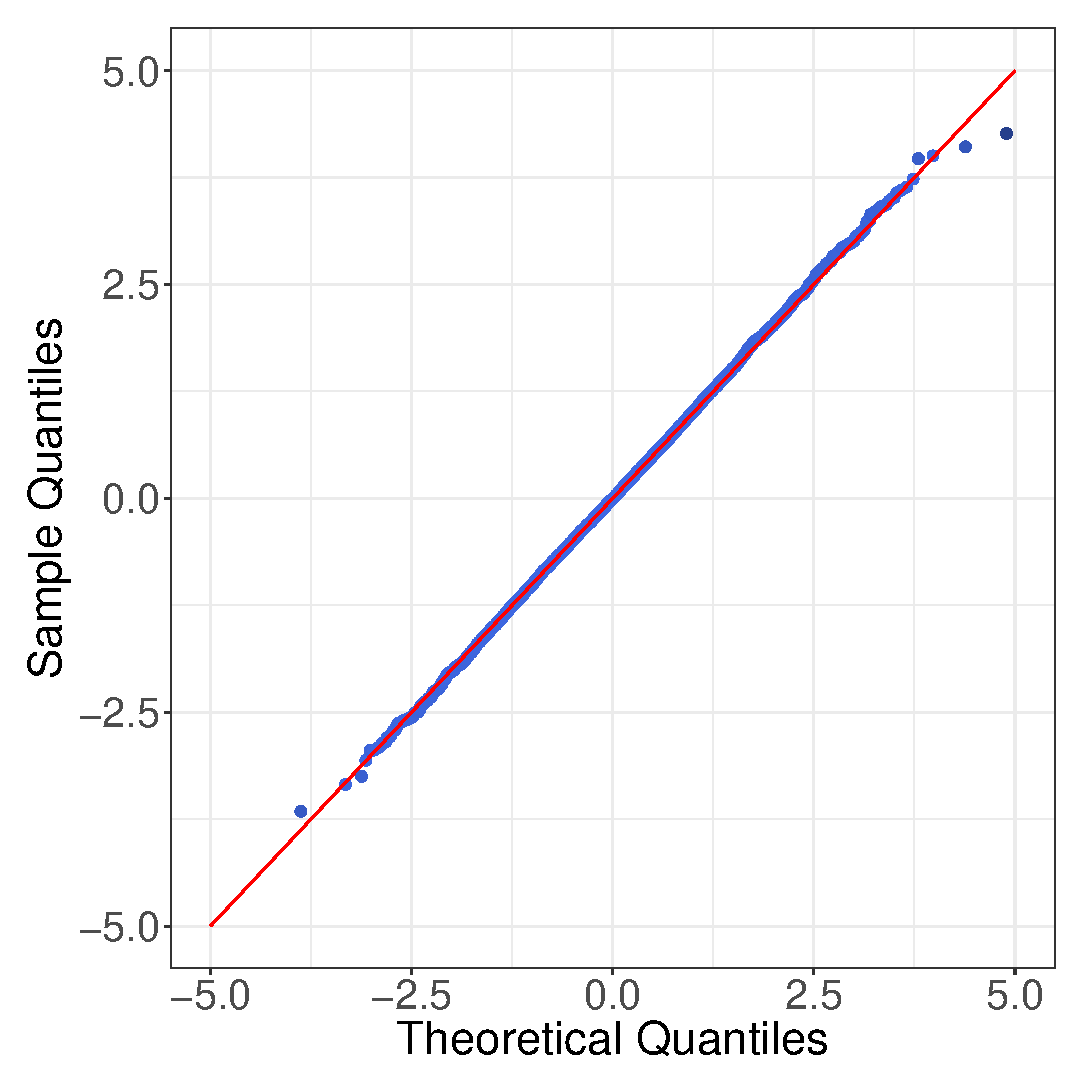
\includegraphics[width=0.3\textwidth]{figure/qqplot/2n50p200}
    }
    \subfigure[$n_1=n_2=50$, $p=500$.]{
        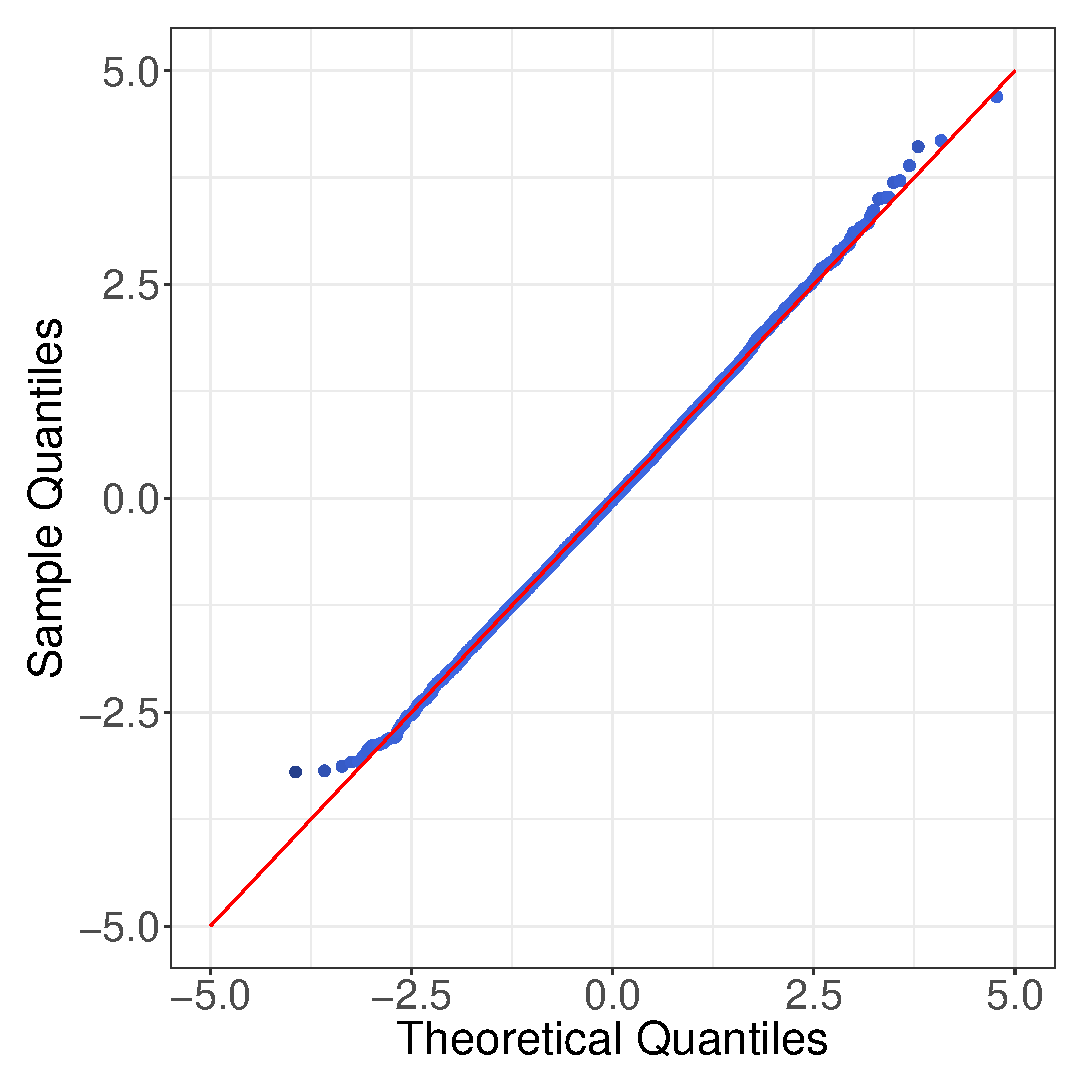
\includegraphics[width=0.3\textwidth]{figure/qqplot/2n50p500}
    }
    \subfigure[$n_1=n_2=50$, $p=800$.]{
        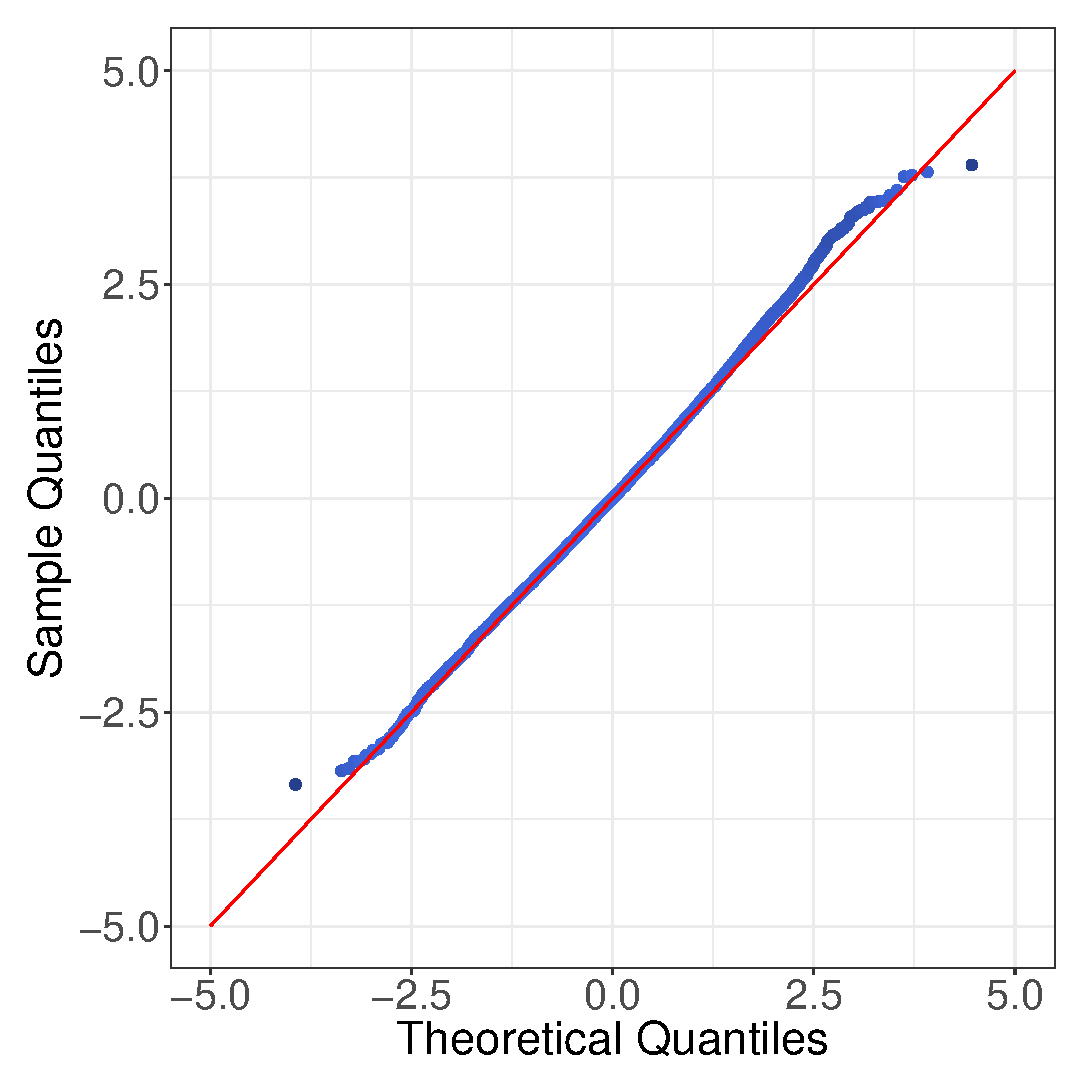
\includegraphics[width=0.3\textwidth]{figure/qqplot/2n50p800}
    }
    \\
    \subfigure[$n_1=n_2=100$, $p=200$.]{
        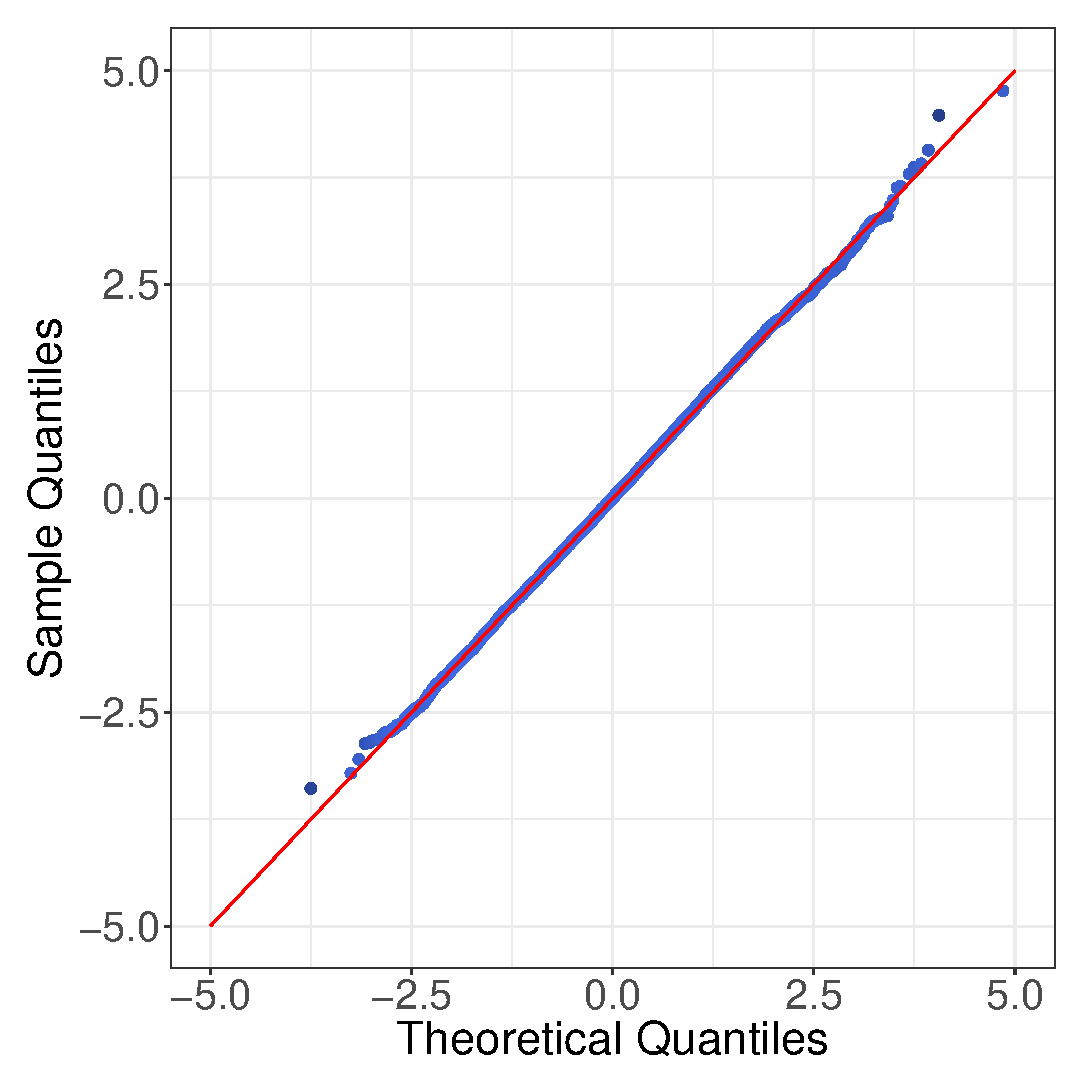
\includegraphics[width=0.3\textwidth]{figure/qqplot/2n100p200}
    }
    \subfigure[$n_1=n_2=100$, $p=500$.]{
        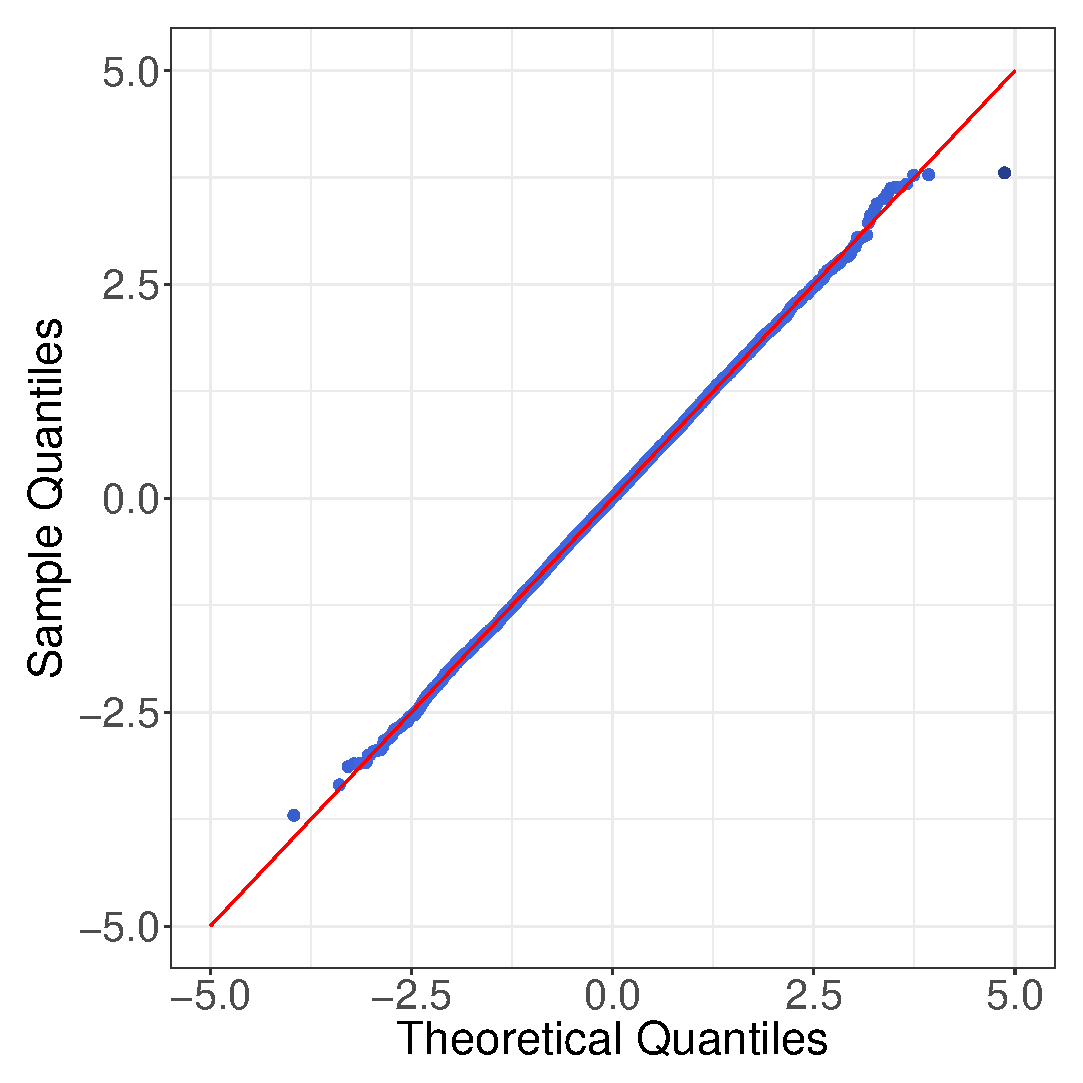
\includegraphics[width=0.3\textwidth]{figure/qqplot/2n100p500}
    }
    \subfigure[$n_1=n_2=100$, $p=800$.]{
        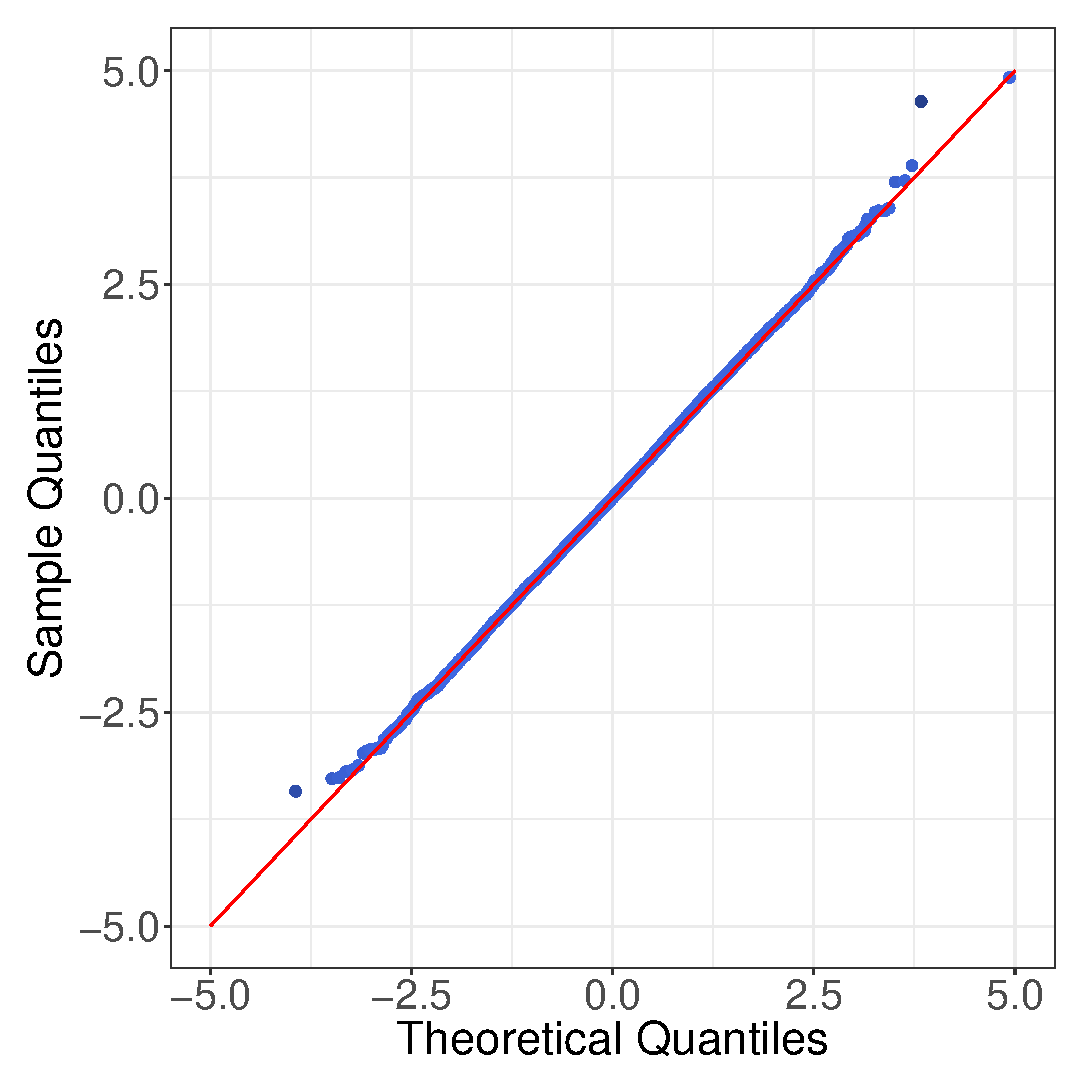
\includegraphics[width=0.3\textwidth]{figure/qqplot/2n100p800}
    }
    \\
    \subfigure[$n_1=n_2=150$, $p=200$.]{
        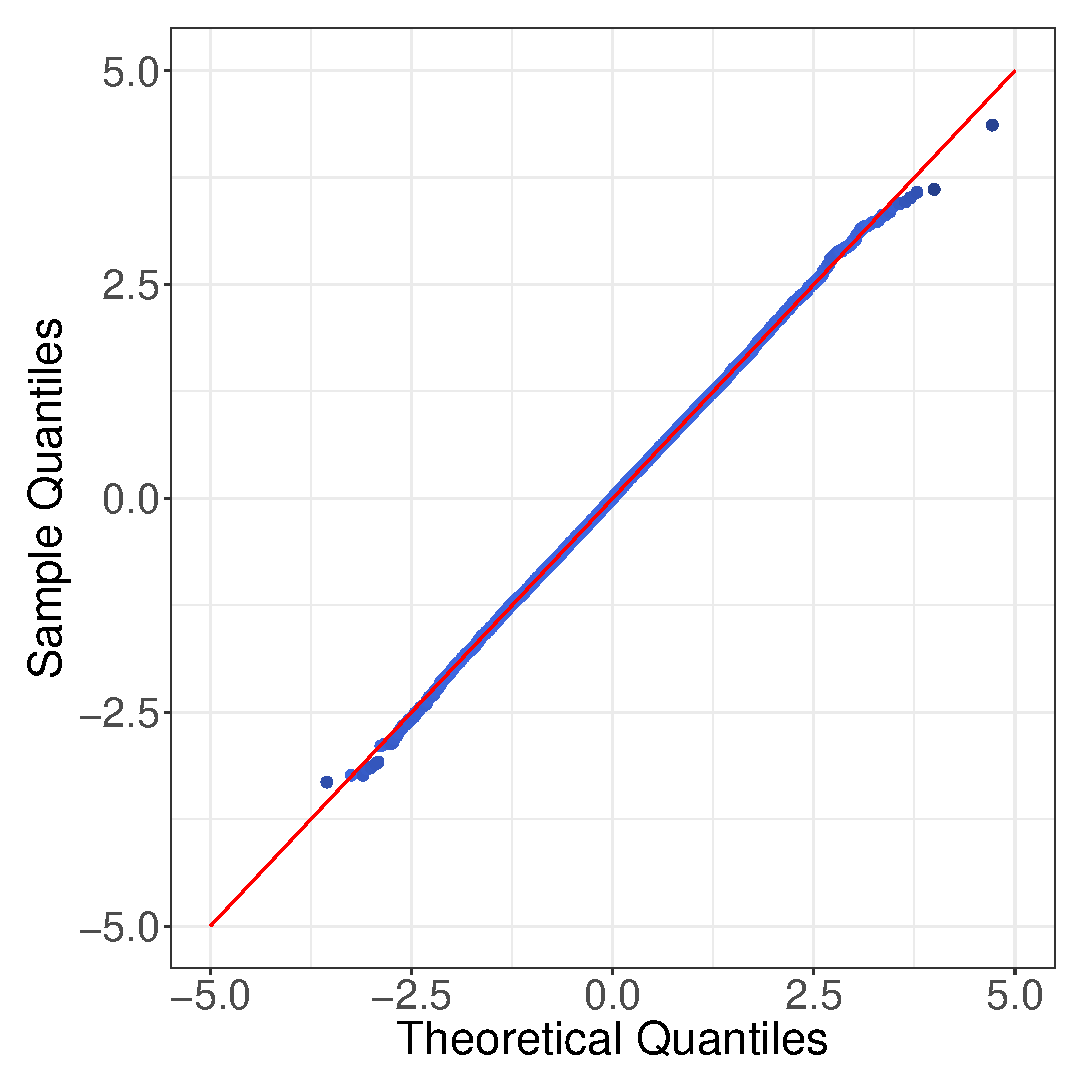
\includegraphics[width=0.3\textwidth]{figure/qqplot/2n150p200}
    }
    \subfigure[$n_1=n_2=150$, $p=500$.]{
        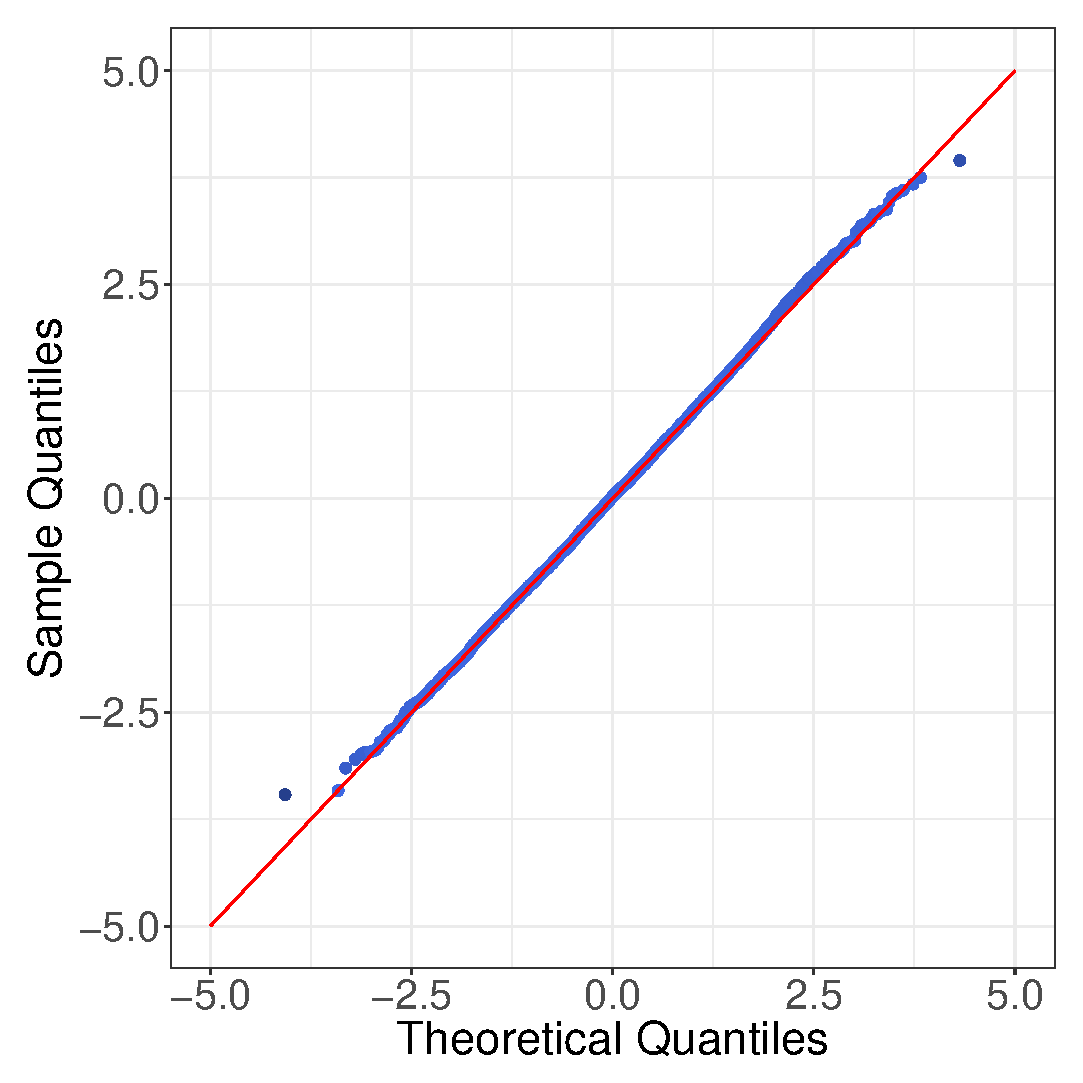
\includegraphics[width=0.3\textwidth]{figure/qqplot/2n150p500}
    }
    \subfigure[$n_1=n_2=150$, $p=800$.]{
        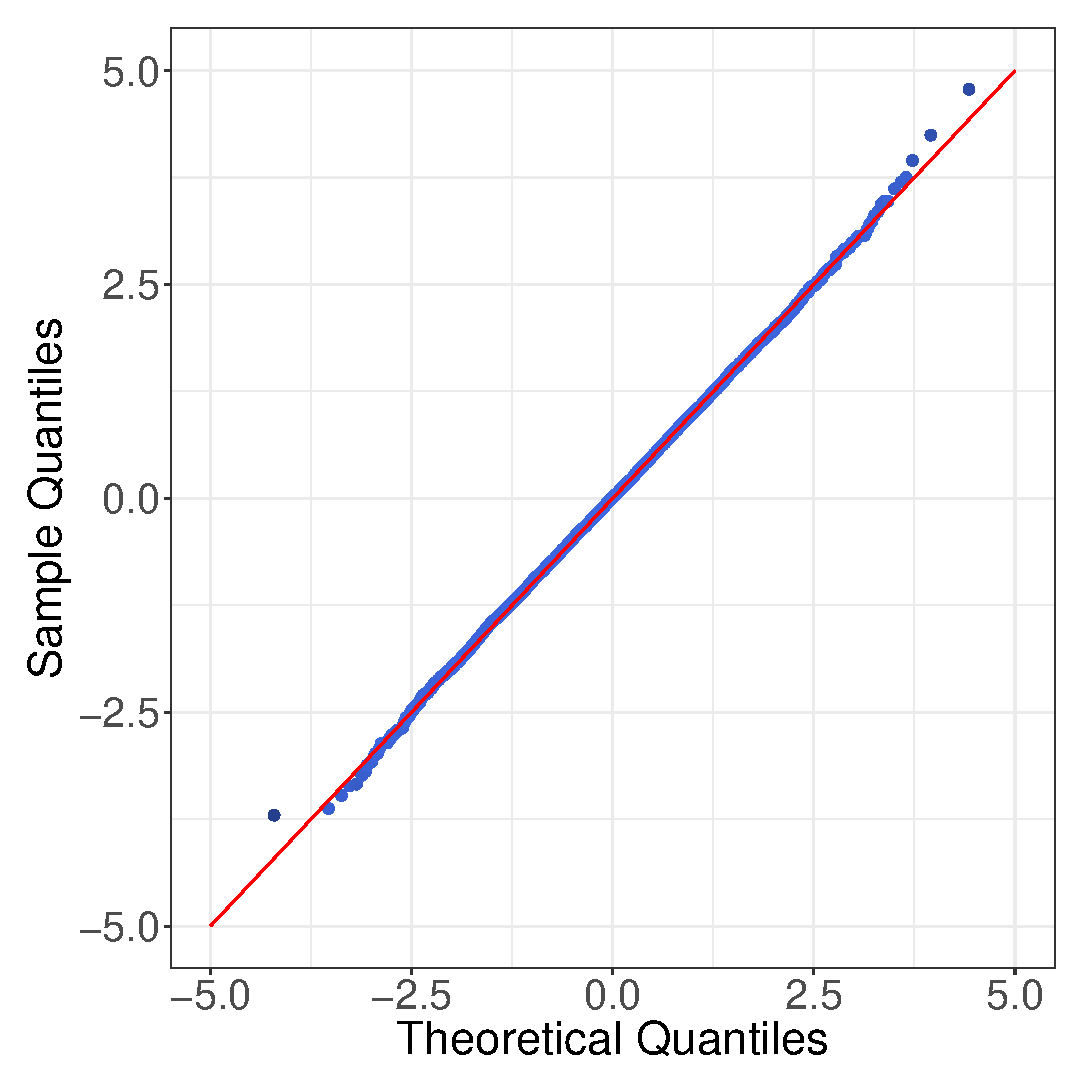
\includegraphics[width=0.3\textwidth]{figure/qqplot/2n150p800}
    }
    \caption{Q-Q plots of the empirical distribution of $Q$ against that of $\{\chi^2(p-r)-(p-r)\}/\sqrt{2(p-r)}$ based on $10000$ independently generated $Q$.
In all cases, $F$ is normal and $\beta=1$.
    }\label{fig:QQ}
\end{figure}

\begin{figure}
    \centering 
    \subfigure[Normal. $\beta=1/2$.]{
        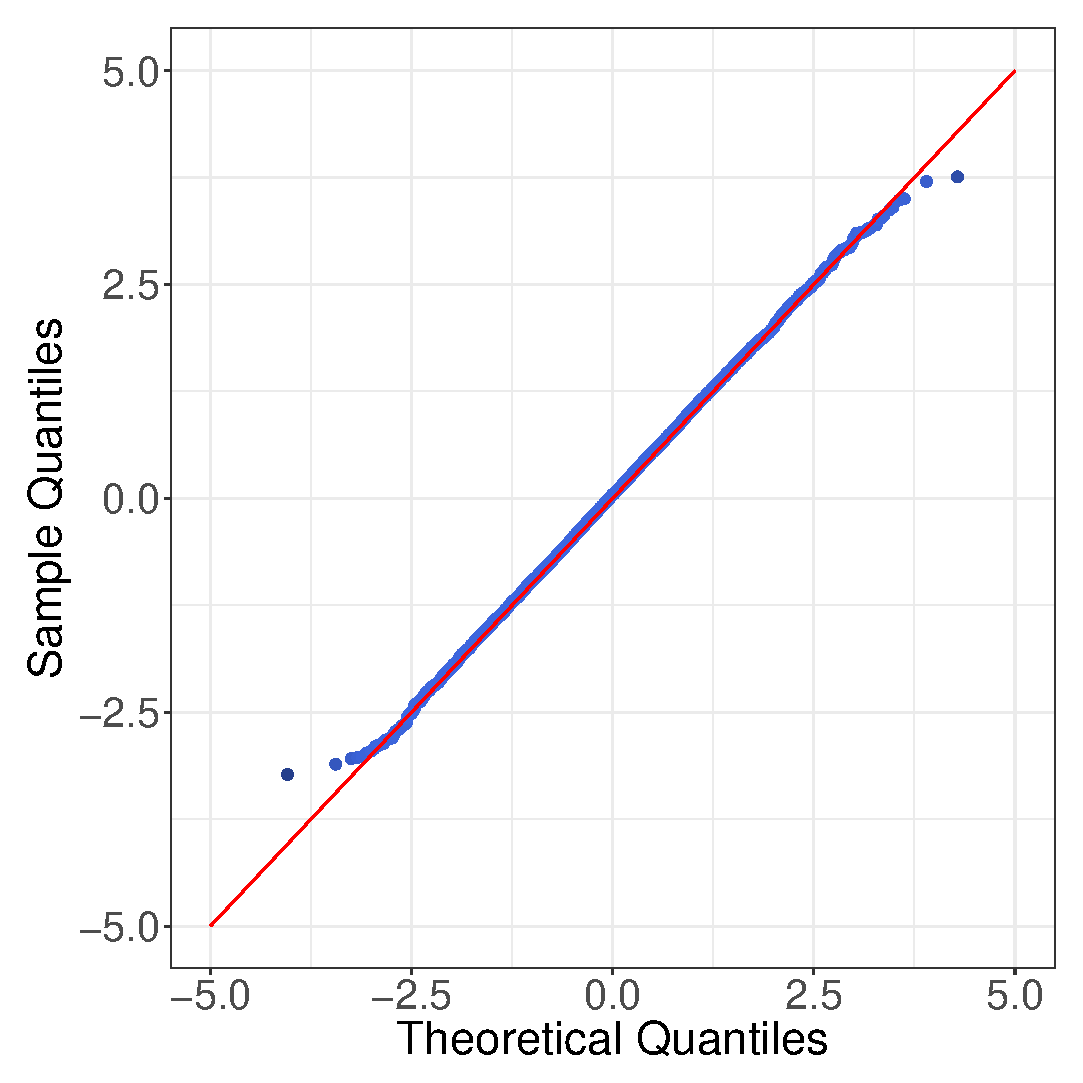
\includegraphics[width=0.3\textwidth]{figure/qqplot/1normal05}
    }
    \subfigure[Normal. $\beta=1$.]{
        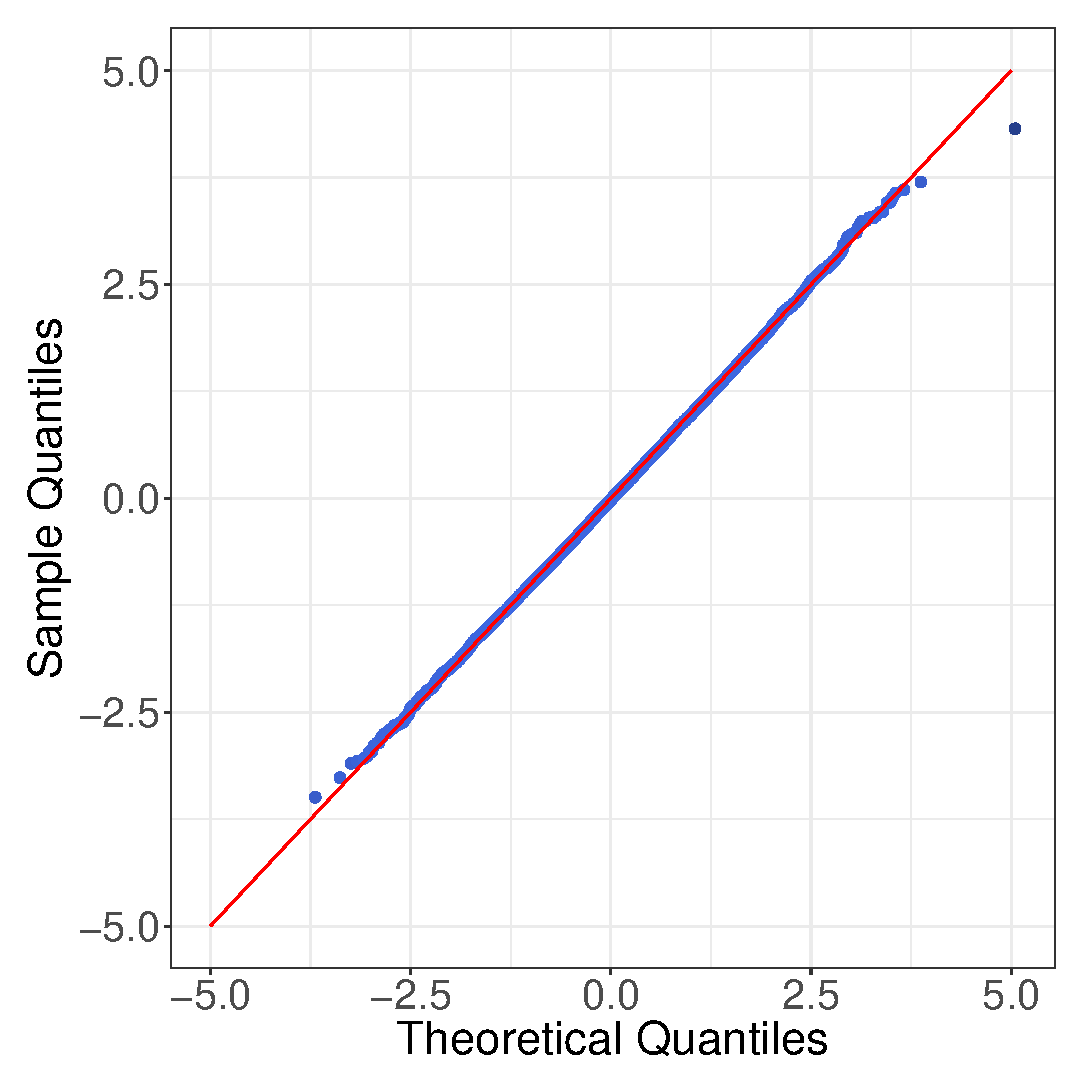
\includegraphics[width=0.3\textwidth]{figure/qqplot/1normal1}
    }
    \subfigure[Normal. $\beta=2$.]{
        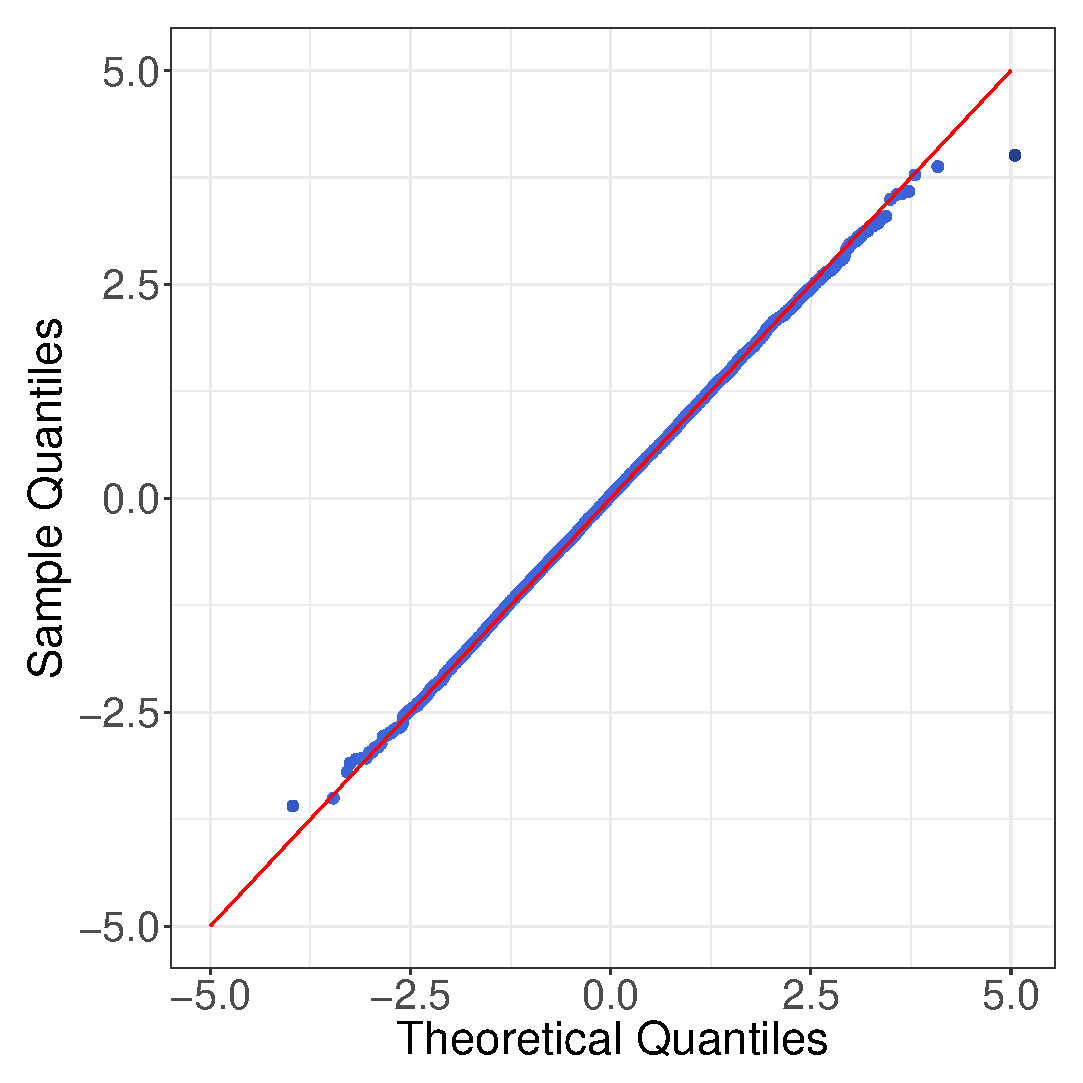
\includegraphics[width=0.3\textwidth]{figure/qqplot/1normal2}
    }
    \\
    \subfigure[Chi-squared. $\beta=1/2$.]{
        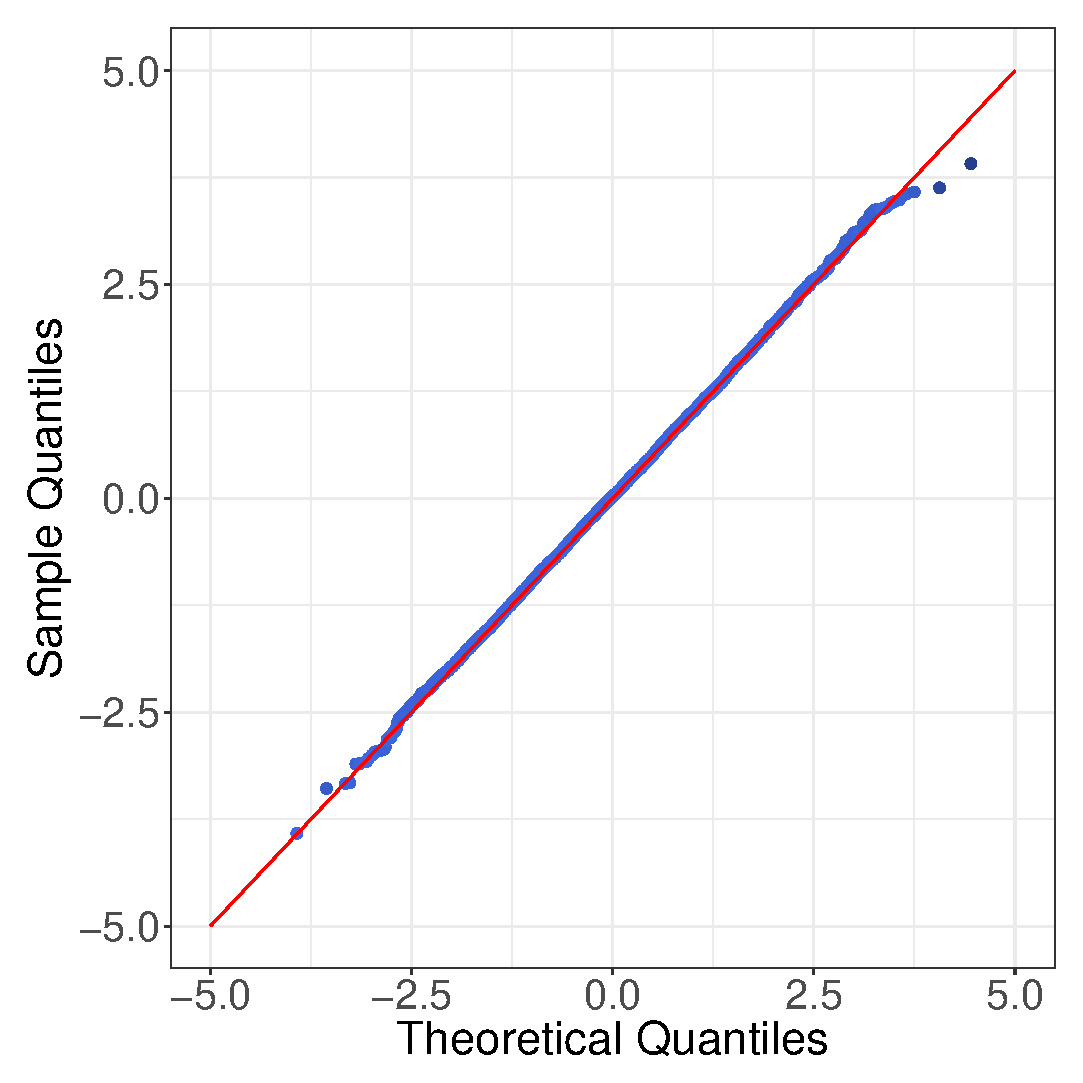
\includegraphics[width=0.3\textwidth]{figure/qqplot/1chiSquared05}
    }
    \subfigure[Chi-squared. $\beta=1$.]{
        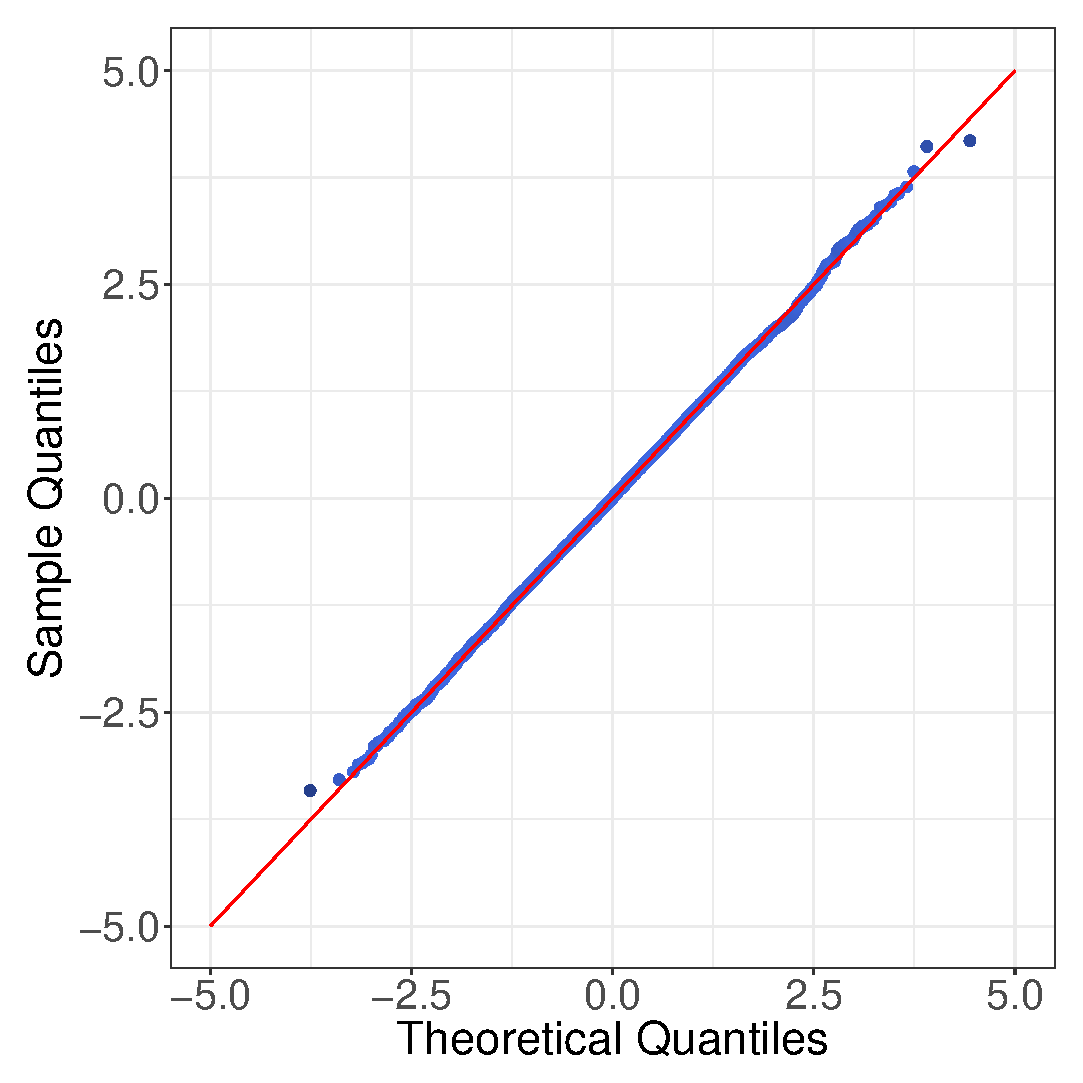
\includegraphics[width=0.3\textwidth]{figure/qqplot/1chiSquared1}
    }
    \subfigure[Chi-squared. $\beta=2$.]{
        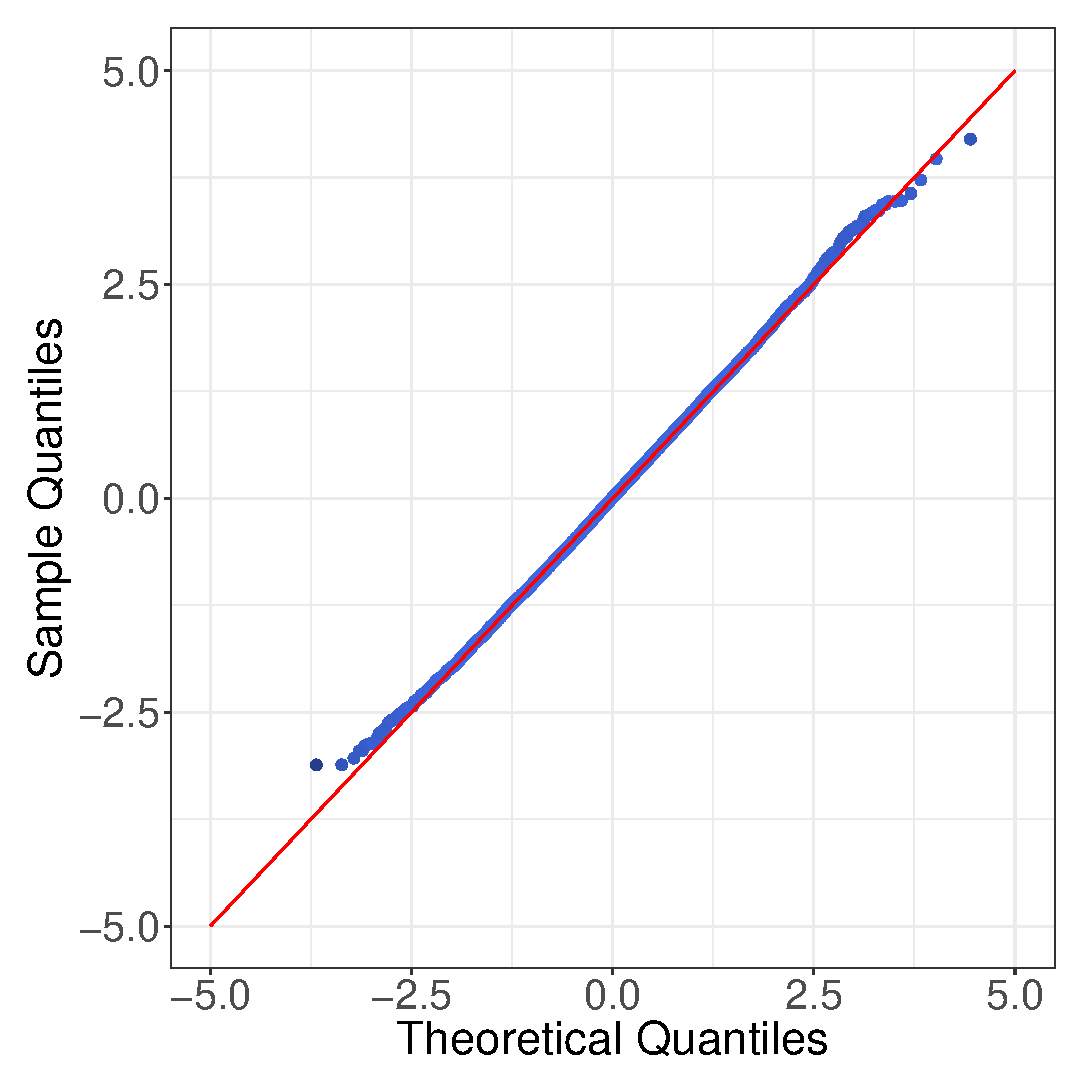
\includegraphics[width=0.3\textwidth]{figure/qqplot/1chiSquared2}
    }
    \\
    \subfigure[Student's $t$. $\beta=1/2$.]{
        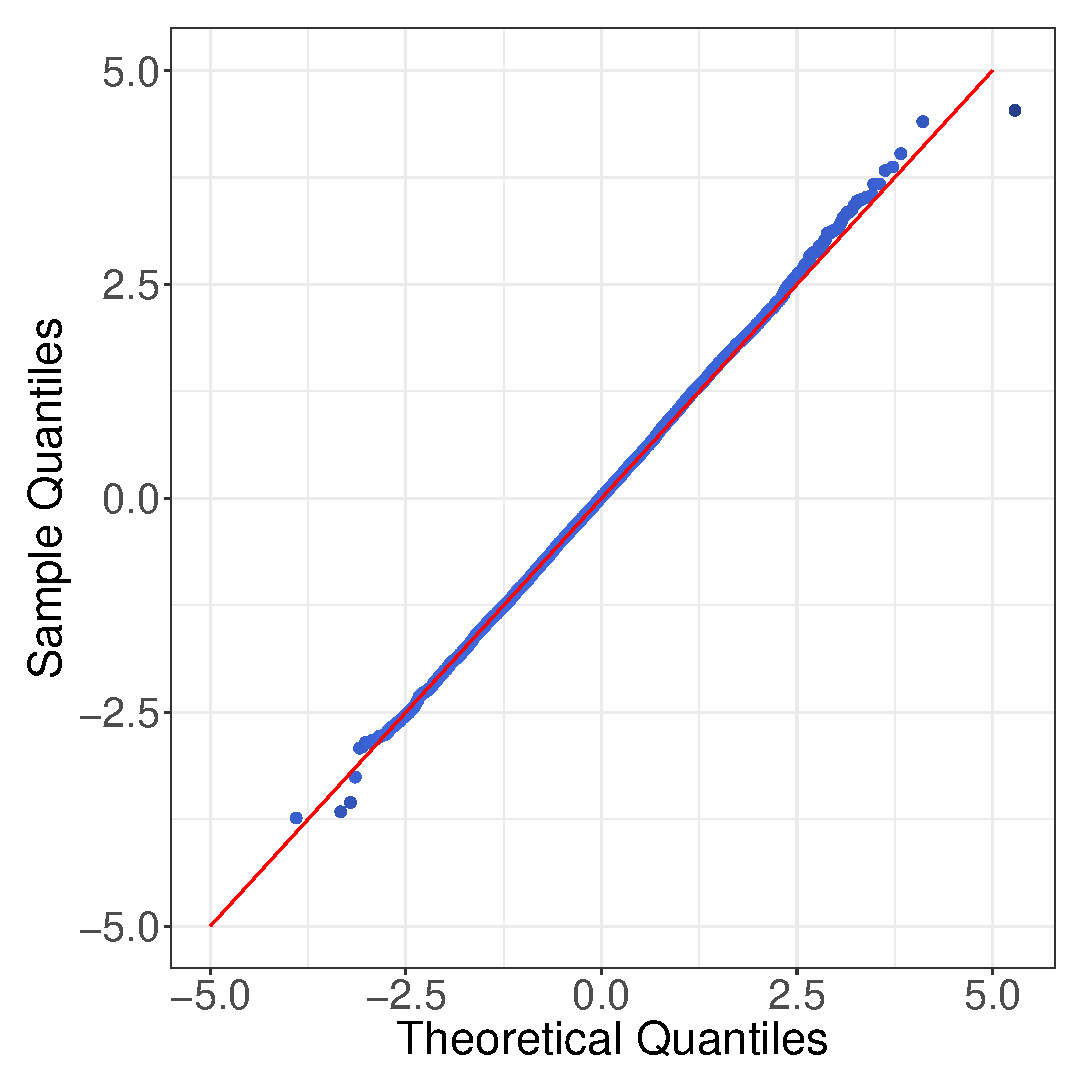
\includegraphics[width=0.3\textwidth]{figure/qqplot/1t05}
    }
    \subfigure[Student's $t$. $\beta=1$.]{
        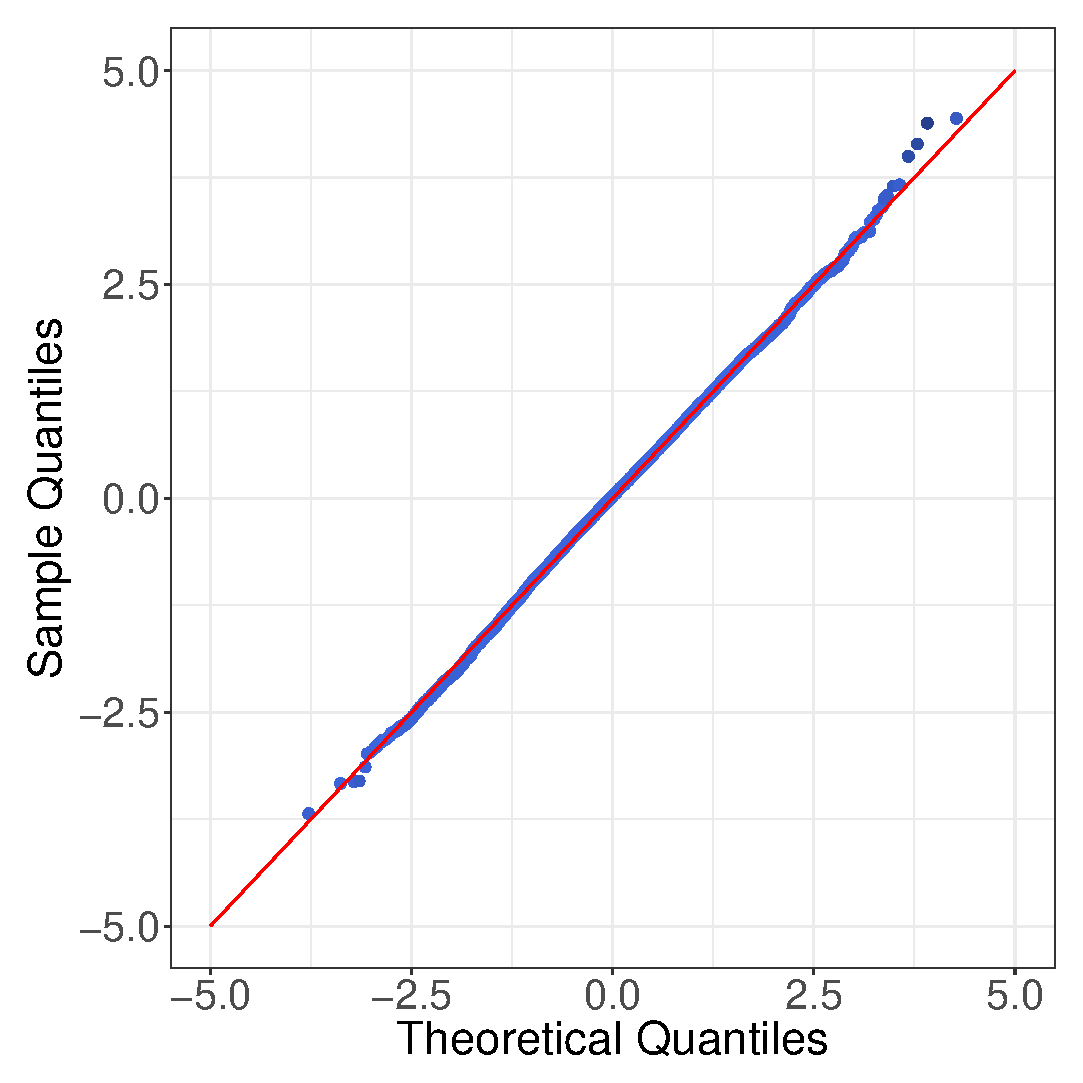
\includegraphics[width=0.3\textwidth]{figure/qqplot/1t1}
    }
    \subfigure[Student's $t$. $\beta=2$.]{
        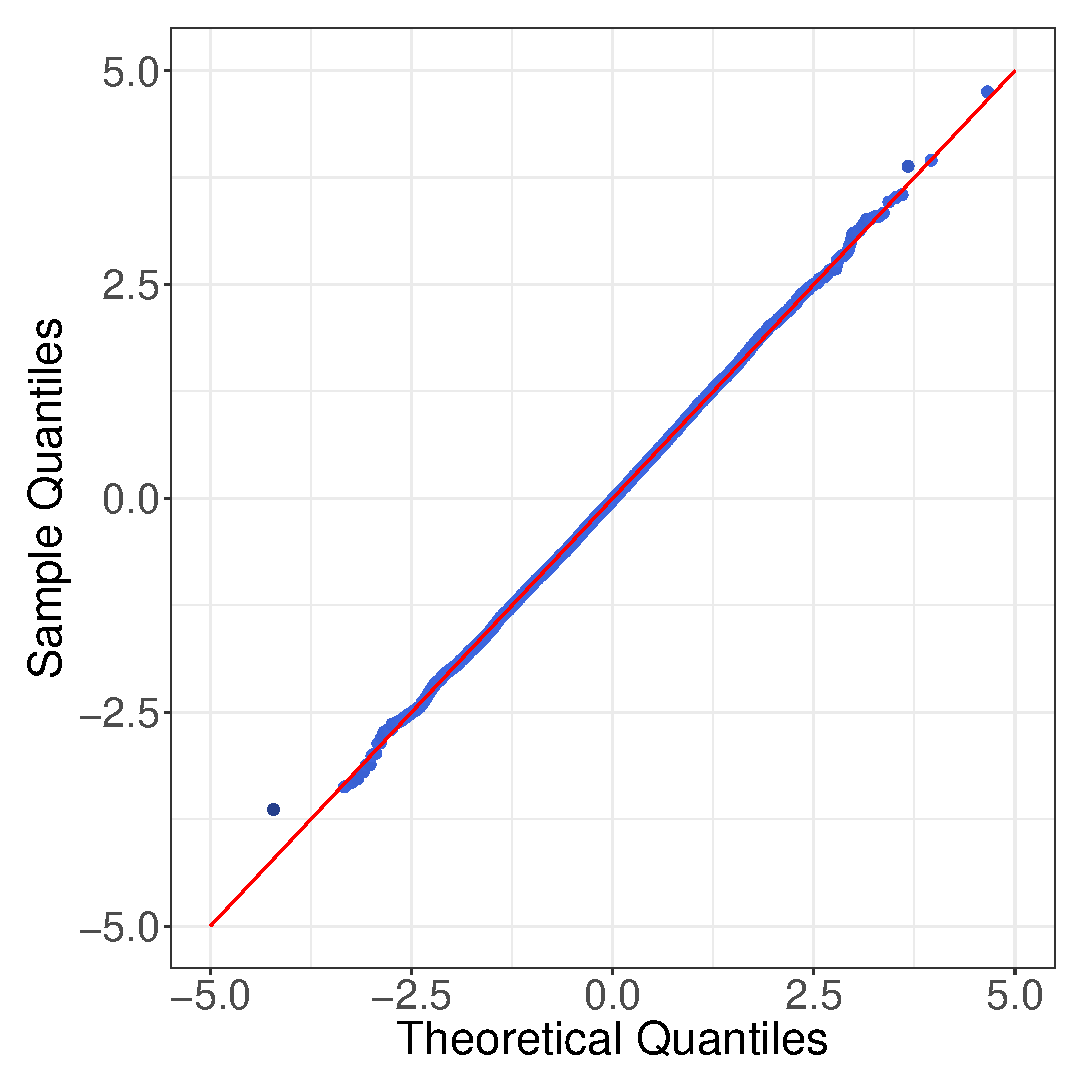
\includegraphics[width=0.3\textwidth]{figure/qqplot/1t2}
    }
    \\
    \caption{Q-Q plots of the empirical distribution of $Q$ against that of $\{\chi^2(p-r)-(p-r)\}/\sqrt{2(p-r)}$ based on $10000$ independently generated $Q$. In all cases, $n_1=n_2=100$ and $p=500$.
    }\label{fig:QQ2}
\end{figure}



Next, we consider the empirical level of the proposed test and compare them with several other alternatives: (1) The corrected $T_{CQ}$ test procedure constructed in Section~\ref{sec:chen} (CCQ); (2) Ma {et al.}~\cite{Ma2015A}'s test (FAST); (3) Chen and Qin~\cite{Chen2010A}'s test (CQ); (4) Srivastava and Du~\cite{Srivastava2008A}'s test (SD); (5) Lopes {\rm et al.}~\cite{Lopes2015A}'s test (LJW).
Samples are repeatedly generated $2000$ times to calculate empirical level.
The results are listed in Tables~\ref{hahaha1}-\ref{hahaha3}.
We can see that the empirical levels of the CQ test are larger than the nominal level in all cases.
The empirical levels of the SD test are close to the nominal level when $\beta=1/2$, but tend to be smaller than the nominal level as $\beta$ increases.
 The empirical levels of the LJW test are very close to the nominal level.
 This is not surprising since the LJW test is exact under the normal distribution.
The empirical levels of the FAST test are very close to the nominal level in most cases, but tend to be smaller than the nominal level when $n_1=n_2=50$, $p=800$ and $\beta=1/2$.
The empirical levels of the CCQ test are very close to the nominal level in all cases.
The empirical levels of the proposed test are a little inflated for $n_1=n_2=50$, but converge to the nominal level as the sample size increases.

% latex table generated in R 3.3.1 by xtable 1.8-2 package
% Sun Jul 31 01:50:20 2016
\begin{table}[ht]
\caption{Empirical levels of the proposed test and competing tests. $n_1=n_2=50$.} 
\label{hahaha1}
\vspace{3mm}
\centering
\begin{tabular}{llllllllll}
\toprule
    &   \multicolumn{3}{c}{Normal} & \multicolumn{3}{c}{Chi-squared}& \multicolumn{3}{c}{Student's $t$}  \\
    \cmidrule(r){2-4}
\cmidrule(r){5-7}
\cmidrule(r){8-10}
    $p$ & $200$ &  $500$ & $800$ & $200$  & $500$ & $800$ & $200$ & $500$ & $800$ \\ 
\midrule
    $\beta=1/2$\\
NEW & 0.0615 & 0.0555 & 0.0595 & 0.0530 & 0.0560 & 0.0630 & 0.0590 & 0.0610 & 0.0565 \\ 
CCQ & 0.0535 & 0.0525 & 0.0490 & 0.0600 & 0.0495 & 0.0550 & 0.0545 & 0.0480 & 0.0590 \\ 
FAST & 0.0525 & 0.0485 & 0.0290 & 0.0485 & 0.0395 & 0.0395 & 0.0560 & 0.0365 & 0.0325 \\ 
CQ & 0.0630 & 0.0645 & 0.0575 & 0.0675 & 0.0665 & 0.0750 & 0.0630 & 0.0725 & 0.0610 \\ 
SD & 0.0515 & 0.0500 & 0.0440 & 0.0525 & 0.0465 & 0.0580 & 0.0440 & 0.0515 & 0.0405 \\ 
LJW & 0.0535 & 0.0480 & 0.0455 & 0.0510 & 0.0575 & 0.0440 & 0.0440 & 0.0500 & 0.0505 \\ 
    $\beta=1$\\
NEW & 0.0480 & 0.0490 & 0.0530 & 0.0595 & 0.0495 & 0.0560 & 0.0500 & 0.0450 & 0.0525 \\ 
CCQ & 0.0545 & 0.0600 & 0.0580 & 0.0585 & 0.0560 & 0.0520 & 0.0500 & 0.0405 & 0.0520 \\ 
FAST & 0.0505 & 0.0470 & 0.0590 & 0.0500 & 0.0550 & 0.0530 & 0.0560 & 0.0420 & 0.0435 \\ 
CQ & 0.0710 & 0.0785 & 0.0720 & 0.0725 & 0.0775 & 0.0730 & 0.0770 & 0.0715 & 0.0675 \\ 
SD & 0.0200 & 0.0165 & 0.0130 & 0.0225 & 0.0130 & 0.0100 & 0.0215 & 0.0075 & 0.0100 \\ 
LJW & 0.0470 & 0.0520 & 0.0460 & 0.0565 & 0.0470 & 0.0535 & 0.0485 & 0.0440 & 0.0540 \\ 
    $\beta=2$\\
New & 0.0590 & 0.0520 & 0.0535 & 0.0575 & 0.0550 & 0.0570 & 0.0545 & 0.0480 & 0.0500 \\ 
CCQ & 0.0535 & 0.0495 & 0.0620 & 0.0495 & 0.0560 & 0.0565 & 0.0525 & 0.0475 & 0.0500 \\ 
FAST & 0.0540 & 0.0530 & 0.0510 & 0.0500 & 0.0565 & 0.0555 & 0.0520 & 0.0445 & 0.0495 \\ 
CQ & 0.0690 & 0.0760 & 0.0675 & 0.0745 & 0.0665 & 0.0630 & 0.0785 & 0.0745 & 0.0700 \\ 
SD & 0.0060 & 0.0010 & 0.0000 & 0.0045 & 0.0010 & 0.0010 & 0.0055 & 0.0010 & 0.0010 \\ 
LJW & 0.0435 & 0.0500 & 0.0535 & 0.0410 & 0.0450 & 0.0430 & 0.0530 & 0.0500 & 0.0515 \\ 
\bottomrule
\end{tabular}
\end{table}


\begin{table}[ht]
\caption{Empirical levels of the proposed test and competing tests. $n_1=n_2=100$.} 
\label{hahaha2}
\vspace{3mm}
\centering
\begin{tabular}{llllllllll}
\toprule
    &   \multicolumn{3}{c}{Normal} & \multicolumn{3}{c}{Chi-squared}& \multicolumn{3}{c}{Student's $t$}  \\
    \cmidrule(r){2-4}
\cmidrule(r){5-7}
\cmidrule(r){8-10}
    $p$ & $200$ &  $500$ & $800$ & $200$  & $500$ & $800$ & $200$ & $500$ & $800$ \\ 
\midrule
    $\beta=1/2$\\
NEW & 0.0465 & 0.0530 & 0.0585 & 0.0500 & 0.0565 & 0.0520 & 0.0630 & 0.0515 & 0.0570 \\ 
CCQ & 0.0545 & 0.0590 & 0.0450 & 0.0555 & 0.0560 & 0.0535 & 0.0530 & 0.0490 & 0.0525 \\ 
FAST & 0.0510 & 0.0505 & 0.0475 & 0.0660 & 0.0555 & 0.0390 & 0.0480 & 0.0465 & 0.0460 \\ 
CQ & 0.0680 & 0.0610 & 0.0640 & 0.0650 & 0.0575 & 0.0630 & 0.0585 & 0.0705 & 0.0510 \\ 
SD & 0.0580 & 0.0520 & 0.0535 & 0.0560 & 0.0500 & 0.0485 & 0.0410 & 0.0615 & 0.0445 \\ 
LJW & 0.0440 & 0.0440 & 0.0460 & 0.0495 & 0.0470 & 0.0475 & 0.0440 & 0.0450 & 0.0505 \\ 
    $\beta=1$\\
NEW & 0.0600 & 0.0490 & 0.0540 & 0.0480 & 0.0470 & 0.0435 & 0.0570 & 0.0520 & 0.0545 \\ 
CCQ & 0.0560 & 0.0435 & 0.0455 & 0.0560 & 0.0540 & 0.0570 & 0.0545 & 0.0540 & 0.0565 \\ 
FAST & 0.0550 & 0.0500 & 0.0550 & 0.0525 & 0.0415 & 0.0450 & 0.0465 & 0.0450 & 0.0555 \\ 
CQ & 0.0715 & 0.0665 & 0.0880 & 0.0655 & 0.0680 & 0.0730 & 0.0785 & 0.0655 & 0.0740 \\ 
SD & 0.0220 & 0.0135 & 0.0085 & 0.0205 & 0.0140 & 0.0095 & 0.0225 & 0.0115 & 0.0100 \\ 
LJW & 0.0525 & 0.0515 & 0.0485 & 0.0420 & 0.0475 & 0.0475 & 0.0485 & 0.0445 & 0.0465 \\ 
    $\beta=2$\\
NEW & 0.0480 & 0.0500 & 0.0500 & 0.0555 & 0.0550 & 0.0465 & 0.0525 & 0.0495 & 0.0540 \\ 
CCQ & 0.0590 & 0.0580 & 0.0450 & 0.0525 & 0.0425 & 0.0620 & 0.0490 & 0.0500 & 0.0540 \\ 
FAST & 0.0460 & 0.0635 & 0.0580 & 0.0565 & 0.0475 & 0.0525 & 0.0640 & 0.0520 & 0.0455 \\ 
CQ & 0.0855 & 0.0775 & 0.0675 & 0.0615 & 0.0695 & 0.0755 & 0.0750 & 0.0740 & 0.0700 \\ 
SD & 0.0055 & 0.0025 & 0.0015 & 0.0030 & 0.0000 & 0.0005 & 0.0025 & 0.0005 & 0.0005 \\ 
LJW & 0.0480 & 0.0495 & 0.0545 & 0.0410 & 0.0455 & 0.0510 & 0.0535 & 0.0435 & 0.0550 \\ 
\bottomrule
\end{tabular}
\end{table}

\begin{table}[ht]
\caption{Empirical levels of the proposed test and competing tests. $n_1=n_2=150$.} 
\label{hahaha3}
\vspace{3mm}
\centering
\begin{tabular}{llllllllll}
\toprule
    &   \multicolumn{3}{c}{Normal} & \multicolumn{3}{c}{Chi-squared}& \multicolumn{3}{c}{Student's $t$}  \\
    \cmidrule(r){2-4}
\cmidrule(r){5-7}
\cmidrule(r){8-10}
    $p$ & $200$ &  $500$ & $800$ & $200$  & $500$ & $800$ & $200$ & $500$ & $800$ \\ 
\midrule
    $\beta=1/2$\\
NEW & 0.0480 & 0.0555 & 0.0430 & 0.0575 & 0.0535 & 0.0575 & 0.0500 & 0.0545 & 0.0560 \\ 
CCQ & 0.0555 & 0.0510 & 0.0405 & 0.0490 & 0.0525 & 0.0575 & 0.0515 & 0.0560 & 0.0490 \\ 
FAST & 0.0510 & 0.0595 & 0.0510 & 0.0510 & 0.0440 & 0.0530 & 0.0625 & 0.0645 & 0.0495 \\ 
CQ & 0.0655 & 0.0780 & 0.0710 & 0.0720 & 0.0515 & 0.0635 & 0.0565 & 0.0725 & 0.0660 \\ 
SD & 0.0530 & 0.0675 & 0.0600 & 0.0585 & 0.0445 & 0.0585 & 0.0465 & 0.0600 & 0.0560 \\ 
LJW & 0.0540 & 0.0520 & 0.0535 & 0.0545 & 0.0555 & 0.0480 & 0.0470 & 0.0500 & 0.0605 \\ 
    $\beta=1$\\
NEW & 0.0525 & 0.0520 & 0.0550 & 0.0450 & 0.0540 & 0.0520 & 0.0540 & 0.0560 & 0.0530 \\ 
CCQ & 0.0435 & 0.0535 & 0.0510 & 0.0525 & 0.0540 & 0.0455 & 0.0560 & 0.0450 & 0.0560 \\ 
FAST & 0.0430 & 0.0530 & 0.0455 & 0.0495 & 0.0480 & 0.0530 & 0.0545 & 0.0510 & 0.0470 \\ 
CQ & 0.0785 & 0.0690 & 0.0740 & 0.0720 & 0.0695 & 0.0715 & 0.0730 & 0.0795 & 0.0725 \\ 
SD & 0.0265 & 0.0115 & 0.0105 & 0.0220 & 0.0130 & 0.0090 & 0.0145 & 0.0145 & 0.0080 \\ 
LJW & 0.0430 & 0.0605 & 0.0460 & 0.0515 & 0.0580 & 0.0525 & 0.0580 & 0.0595 & 0.0510 \\ 
    $\beta=2$\\
NEW & 0.0340 & 0.0645 & 0.0525 & 0.0550 & 0.0475 & 0.0465 & 0.0540 & 0.0545 & 0.0510 \\ 
CCQ & 0.0505 & 0.0525 & 0.0475 & 0.0520 & 0.0505 & 0.0535 & 0.0525 & 0.0510 & 0.0600 \\ 
FAST & 0.0525 & 0.0415 & 0.0505 & 0.0490 & 0.0560 & 0.0560 & 0.0490 & 0.0400 & 0.0555 \\ 
CQ & 0.0675 & 0.0705 & 0.0695 & 0.0765 & 0.0655 & 0.0775 & 0.0785 & 0.0720 & 0.0875 \\ 
SD & 0.0040 & 0.0020 & 0.0005 & 0.0030 & 0.0000 & 0.0000 & 0.0025 & 0.0010 & 0.0000 \\ 
LJW & 0.0490 & 0.0475 & 0.0490 & 0.0465 & 0.0535 & 0.0480 & 0.0490 & 0.0445 & 0.0490 \\ 
\bottomrule
\end{tabular}
\end{table}


Now we consider the empirical power of the proposed test and competing tests.
In view of Corollary~\ref{testPowerh}, we define the SNR as $\textrm{SNR}=\|\mu_1-\mu_2\|^2/(\sigma^2\sqrt{2\tau^2 p})$.
We take $\mu_1=\mathbf{0}_p$.
The orientation of $\mu_2$ is from the uniform distribution on the unit sphere.
The norm of $\mu_2$ is selected to make SNR equal to specific values.
Samples are repeatedly generated $2000$ times to calculate empirical power.
The simulation results are illustrated in Figures~\ref{fig:Power} and~\ref{fig:Power2}.
From the results, we can see that our test outperforms the other five tests substantially under the spiked covariance model.

\begin{figure}
    \centering 
    \subfigure[$n_1=n_2=50$, $p=200$.]{
        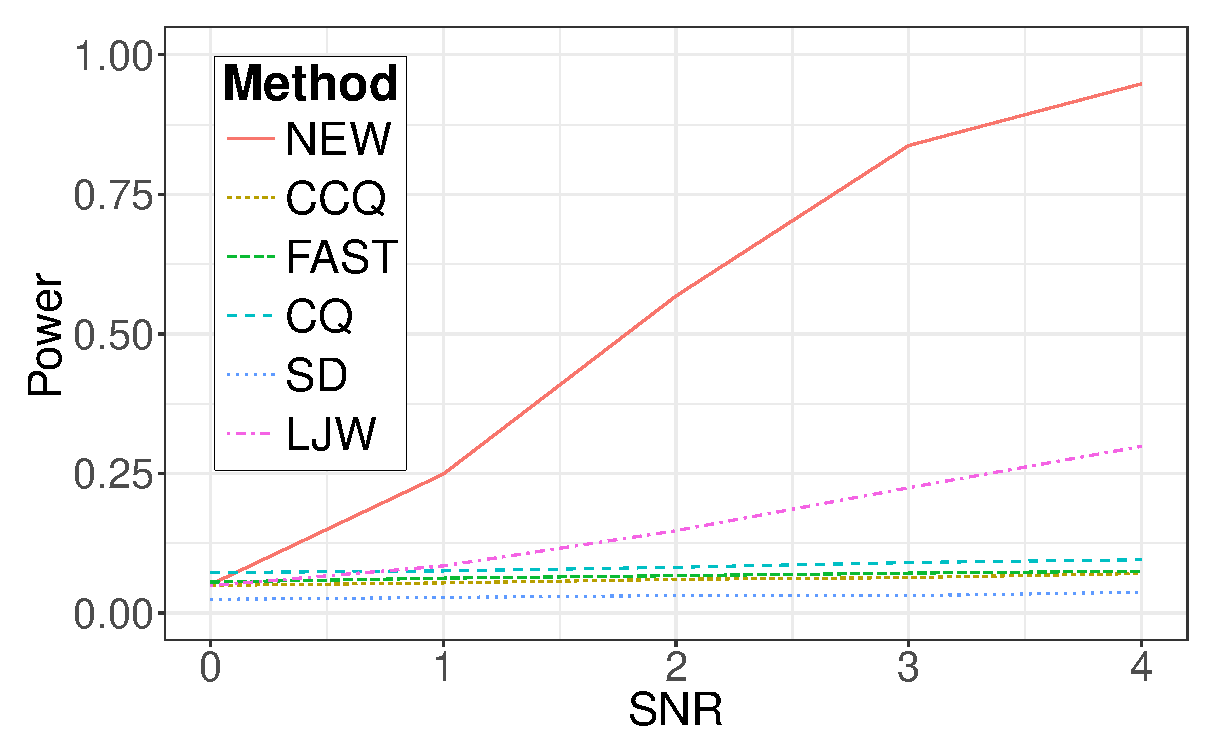
\includegraphics[width=0.3\textwidth]{figure/power/Power2n50p200}
    }
    \subfigure[$n_1=n_2=50$, $p=500$.]{
        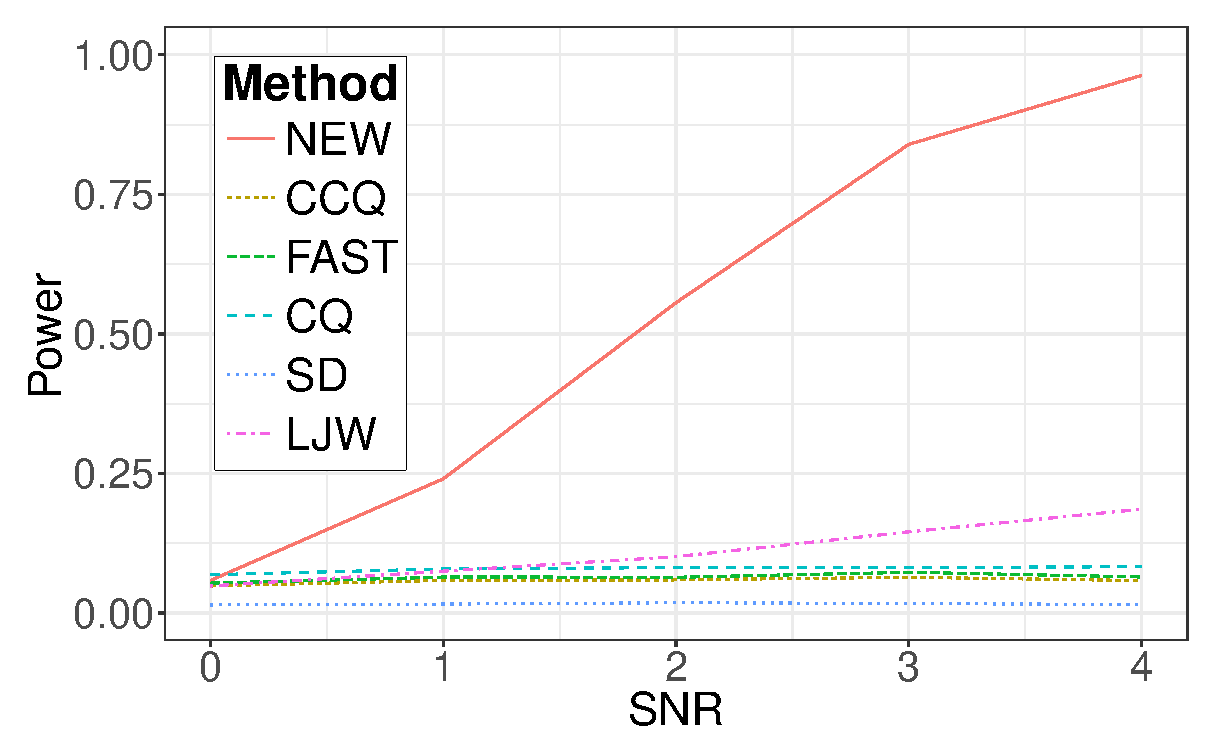
\includegraphics[width=0.3\textwidth]{figure/power/Power2n50p500}
    }
    \subfigure[$n_1=n_2=50$, $p=800$.]{
        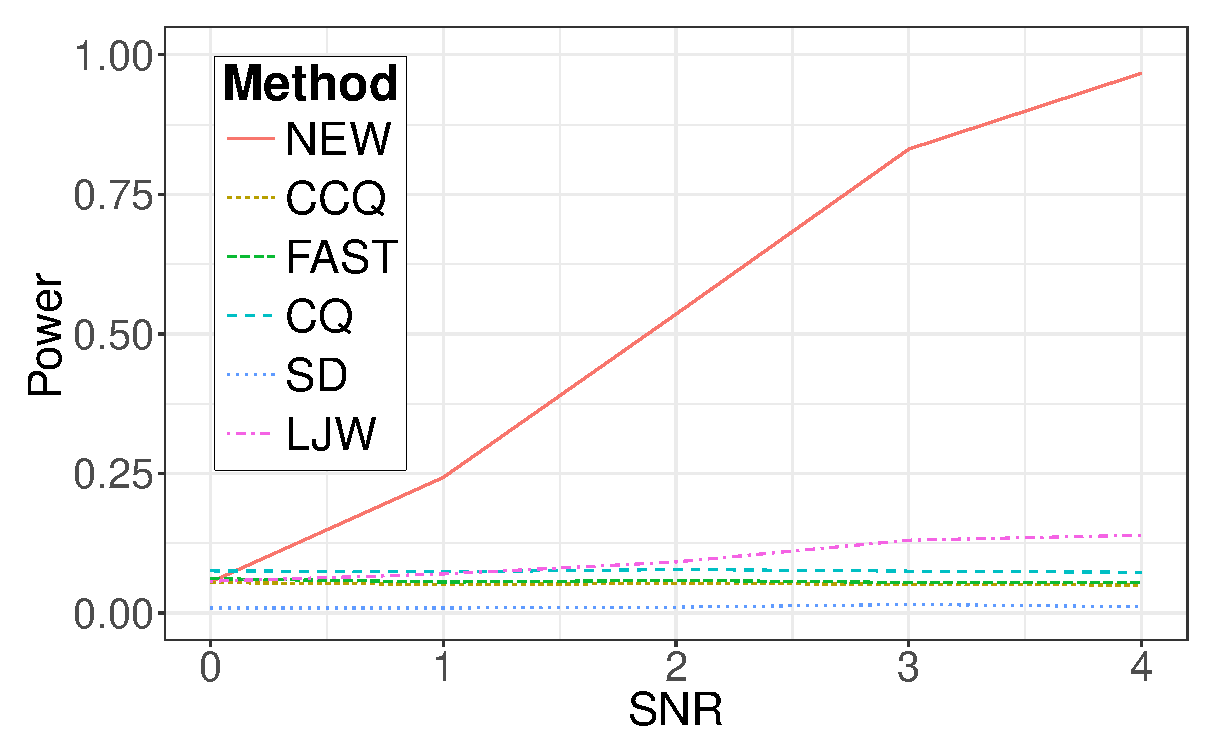
\includegraphics[width=0.3\textwidth]{figure/power/Power2n50p800}
    }
    \\
    \subfigure[$n_1=n_2=100$, $p=200$.]{
        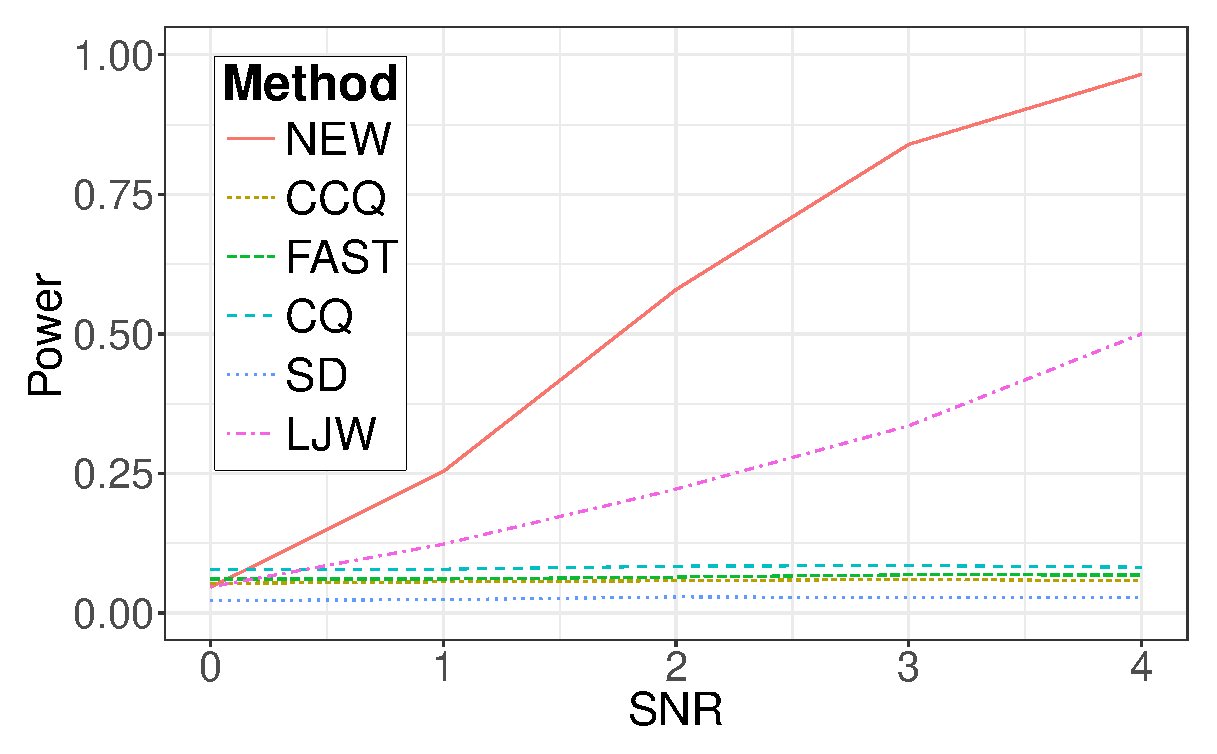
\includegraphics[width=0.3\textwidth]{figure/power/Power2n100p200}
    }
    \subfigure[$n_1=n_2=100$, $p=500$.]{
        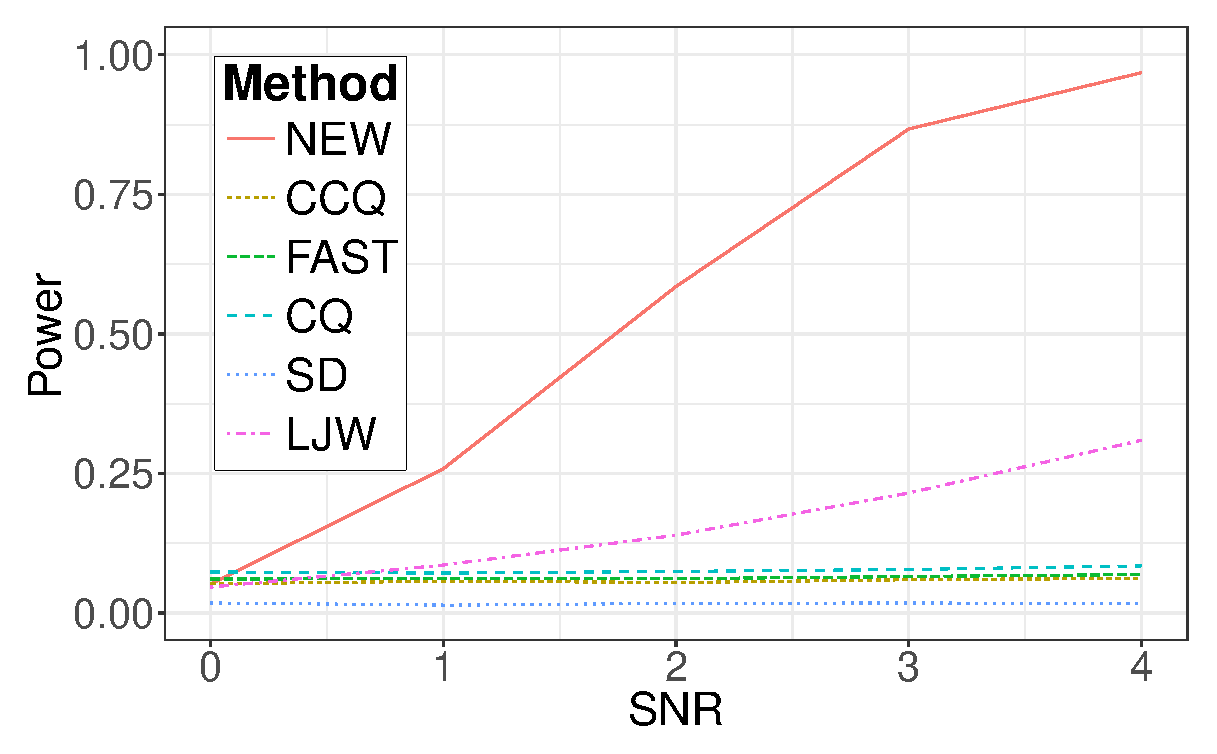
\includegraphics[width=0.3\textwidth]{figure/power/Power2n100p500}
    }
    \subfigure[$n_1=n_2=100$, $p=800$.]{
        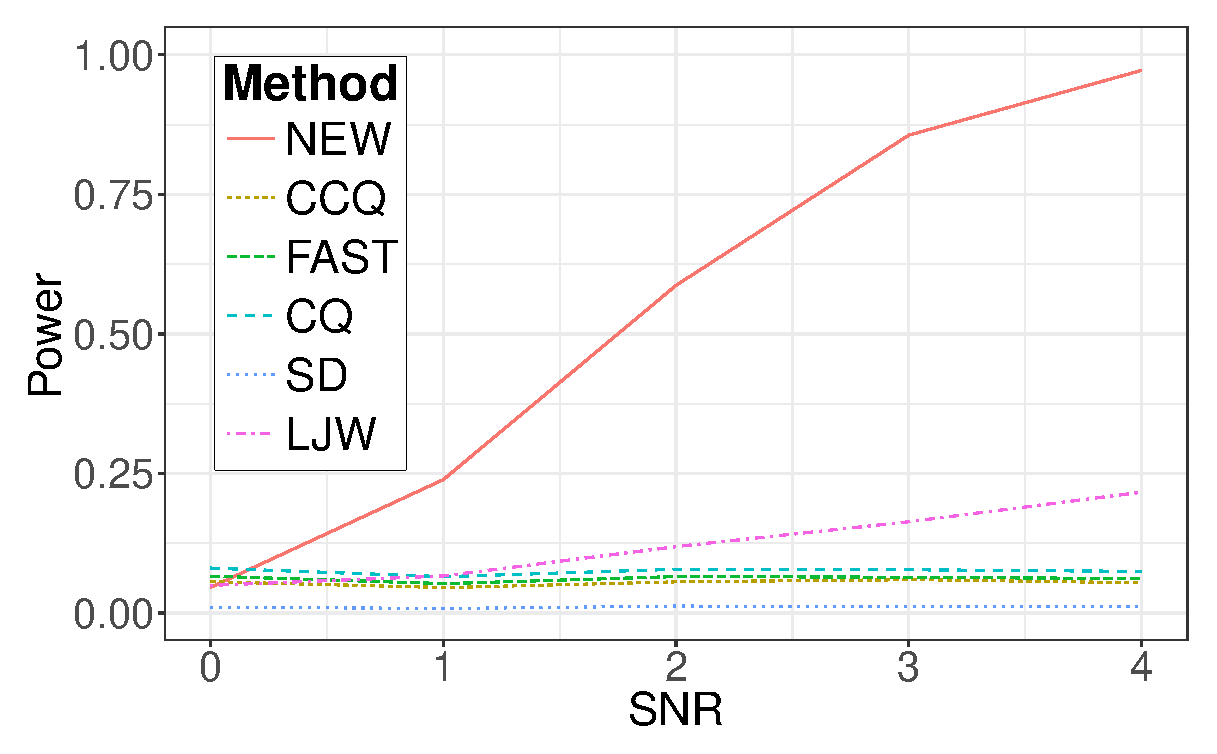
\includegraphics[width=0.3\textwidth]{figure/power/Power2n100p800}
    }
    \\
    \subfigure[$n_1=n_2=150$, $p=200$.]{
        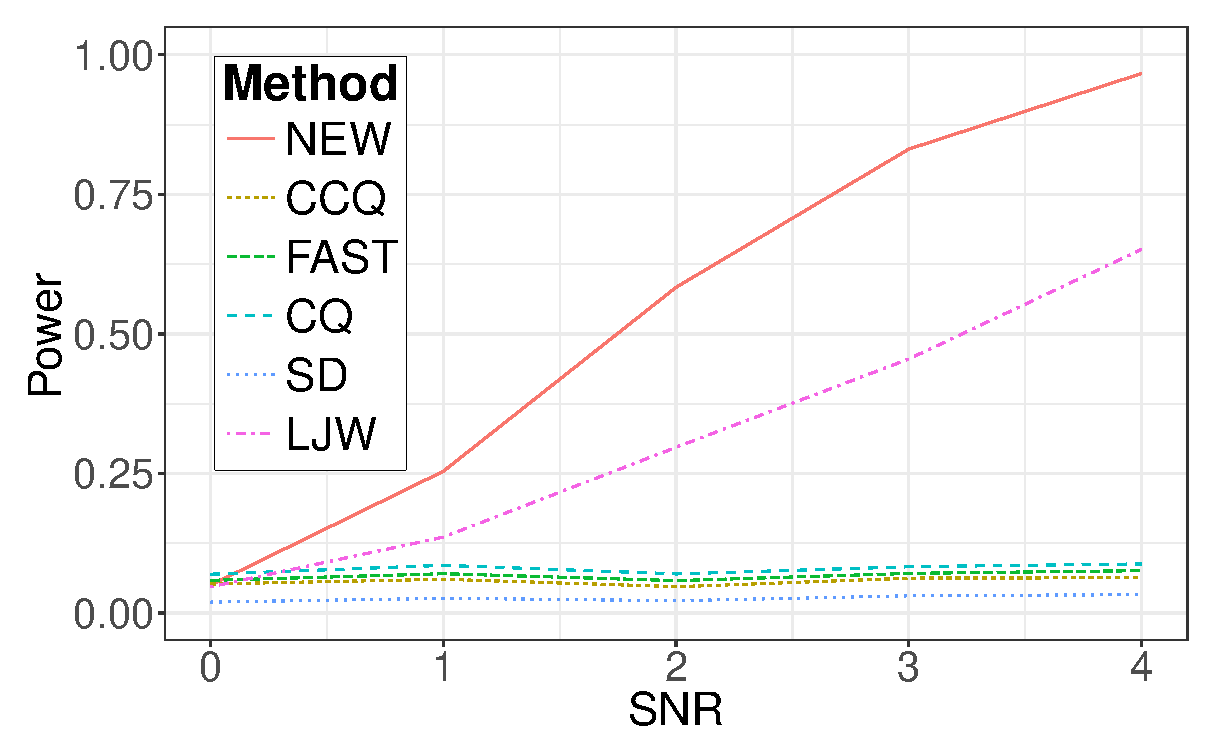
\includegraphics[width=0.3\textwidth]{figure/power/Power2n150p200}
    }
    \subfigure[$n_1=n_2=150$, $p=500$.]{
        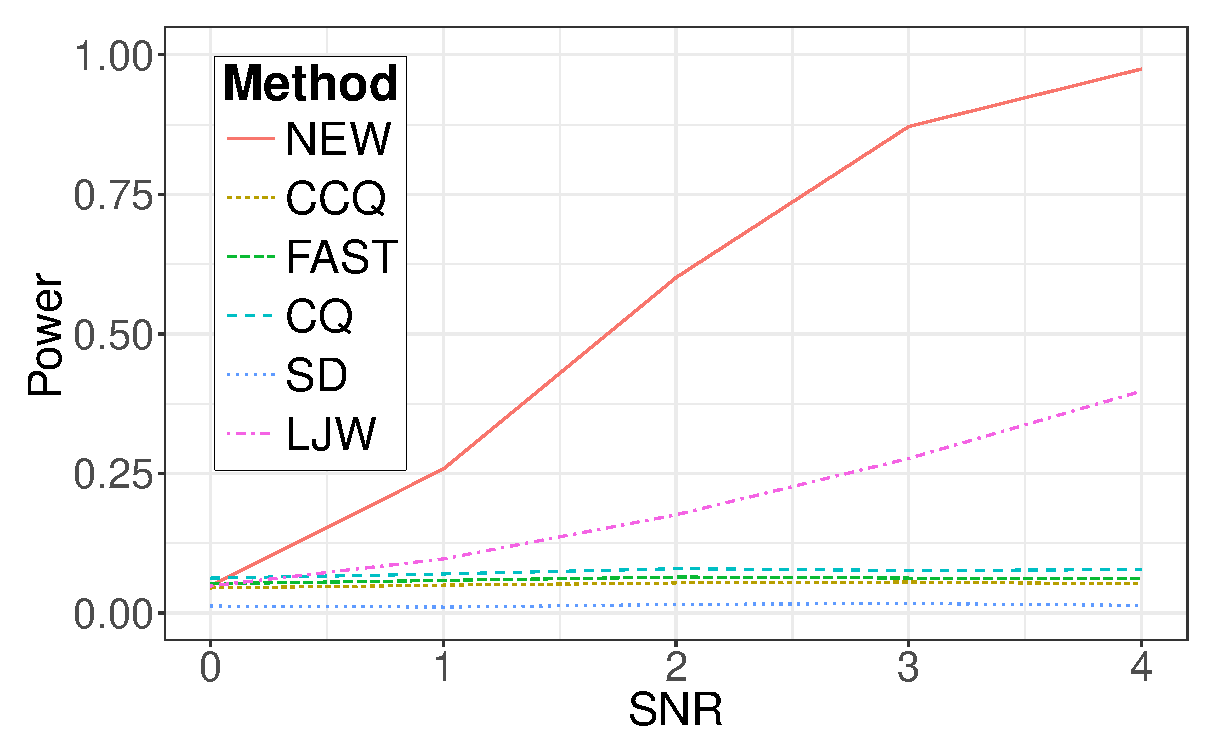
\includegraphics[width=0.3\textwidth]{figure/power/Power2n150p500}
    }
    \subfigure[$n_1=n_2=150$, $p=800$.]{
        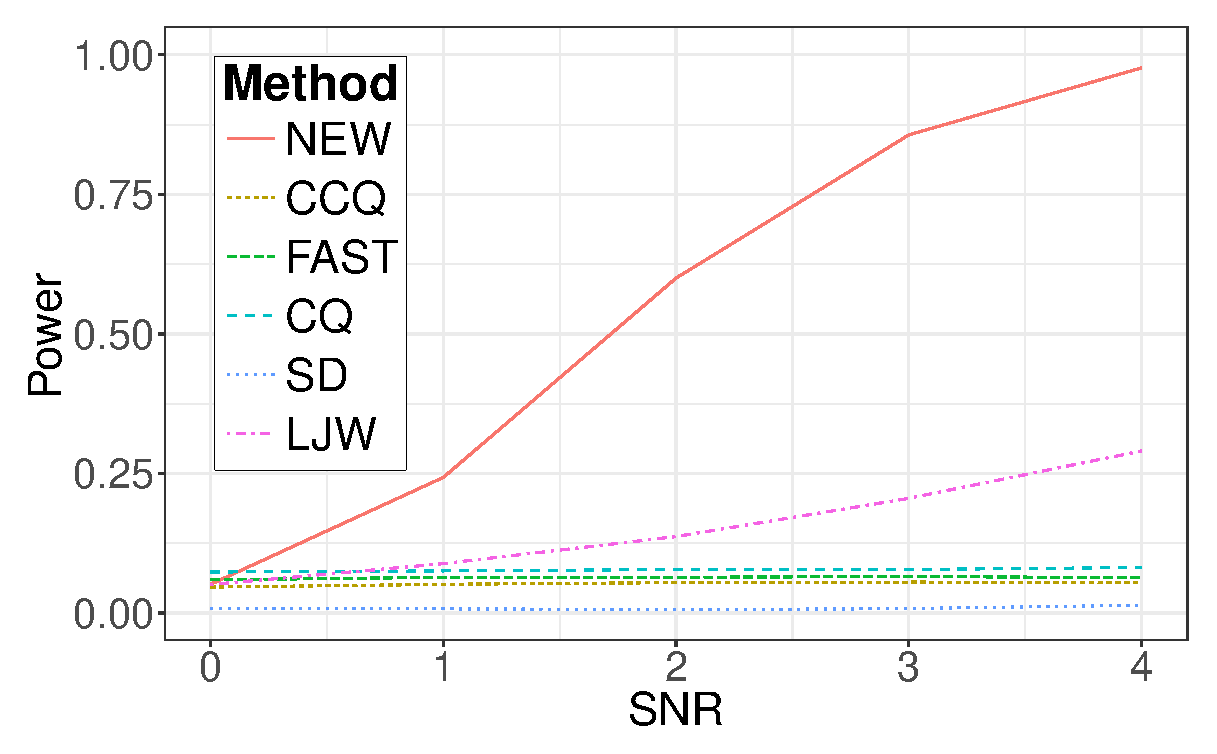
\includegraphics[width=0.3\textwidth]{figure/power/Power2n150p800}
    }
    \caption{Empirical power of our test and competing tests. In all cases, $F$ is normal and $\beta=1$.}\label{fig:Power}
\end{figure}

\begin{figure}
    \centering 
    \subfigure[Normal. $\beta=1/2$.]{
        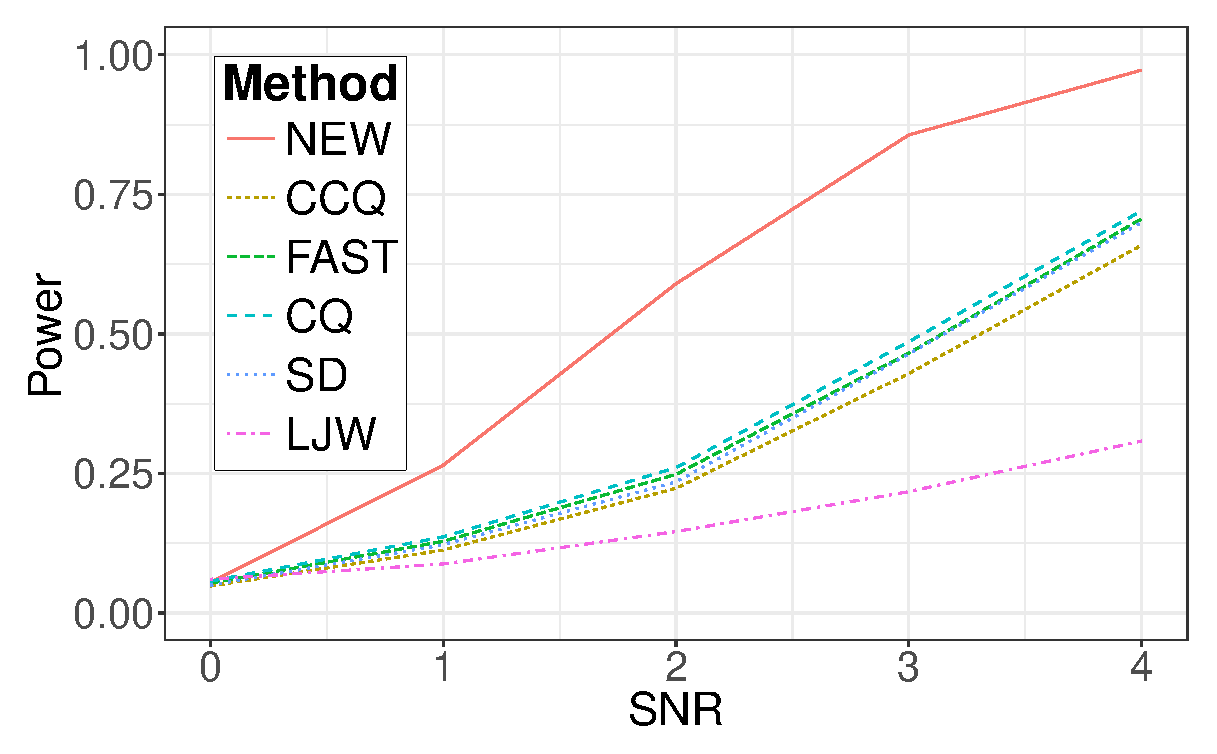
\includegraphics[width=0.3\textwidth]{figure/power/Power1normal05}
    }
    \subfigure[Normal. $\beta=1$.]{
        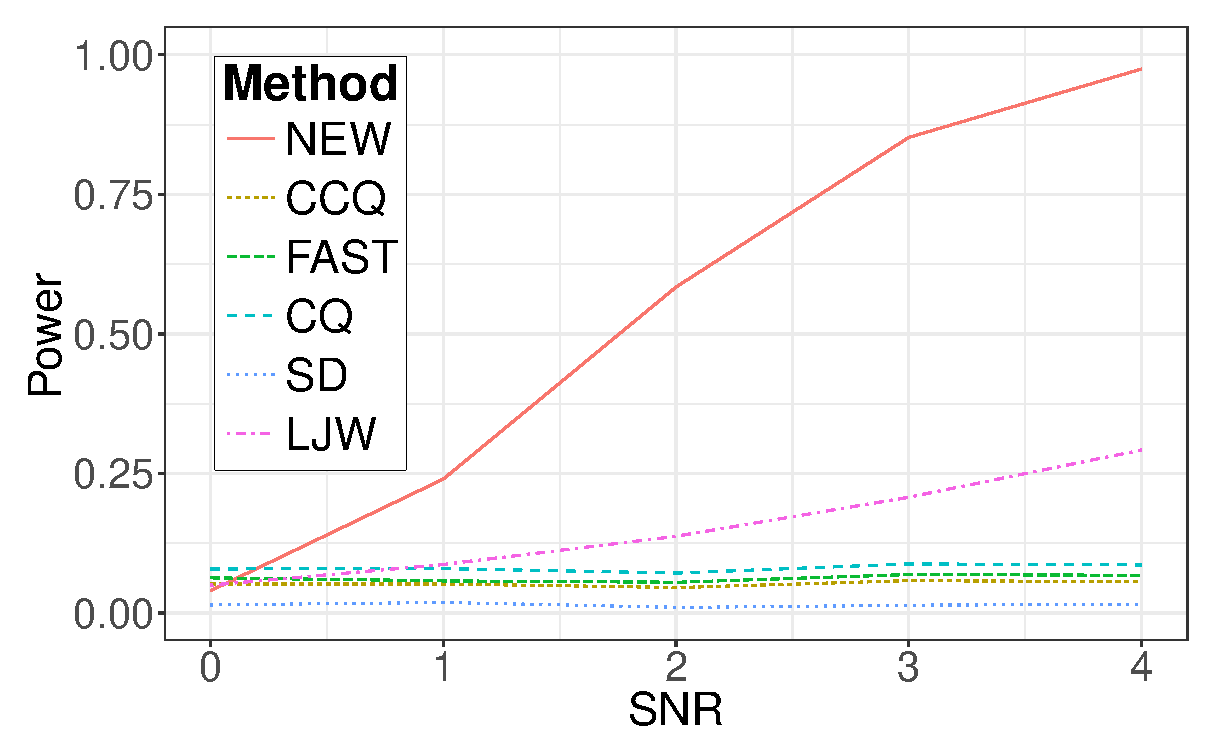
\includegraphics[width=0.3\textwidth]{figure/power/Power1normal1}
    }
    \subfigure[Normal. $\beta=2$.]{
        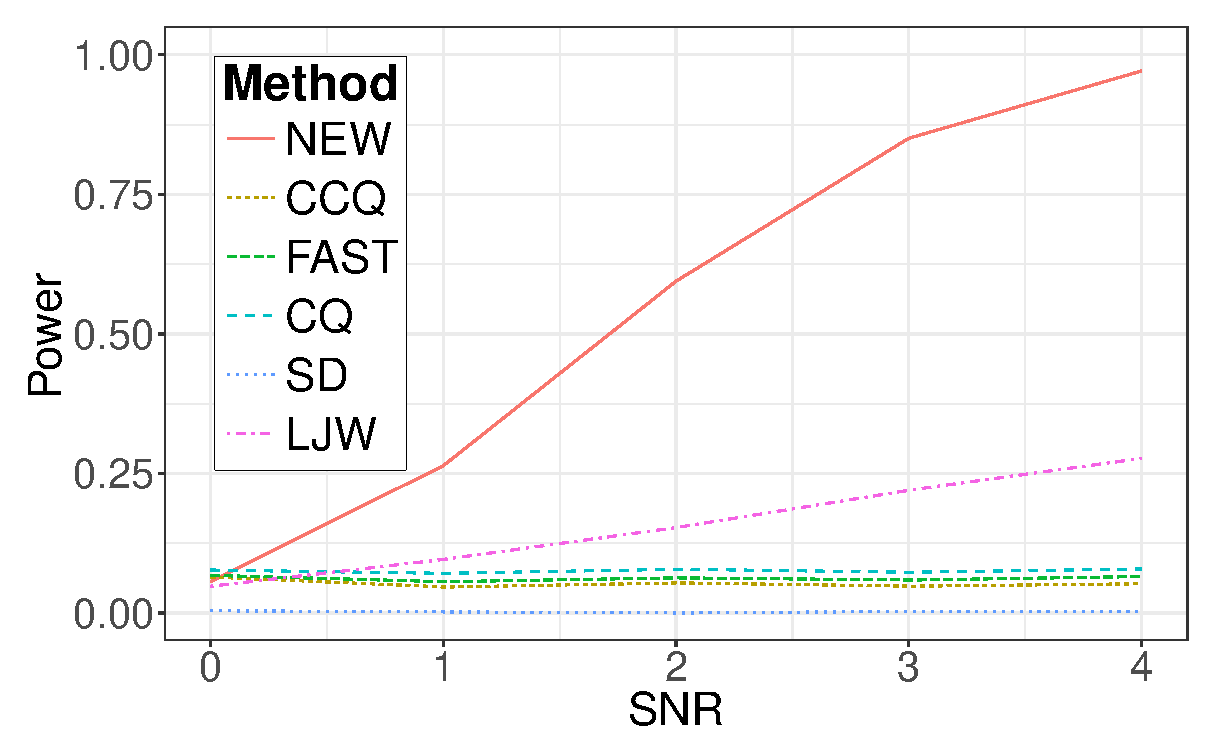
\includegraphics[width=0.3\textwidth]{figure/power/Power1normal2}
    }
    \\
    \subfigure[Chi-squared. $\beta=1/2$.]{
        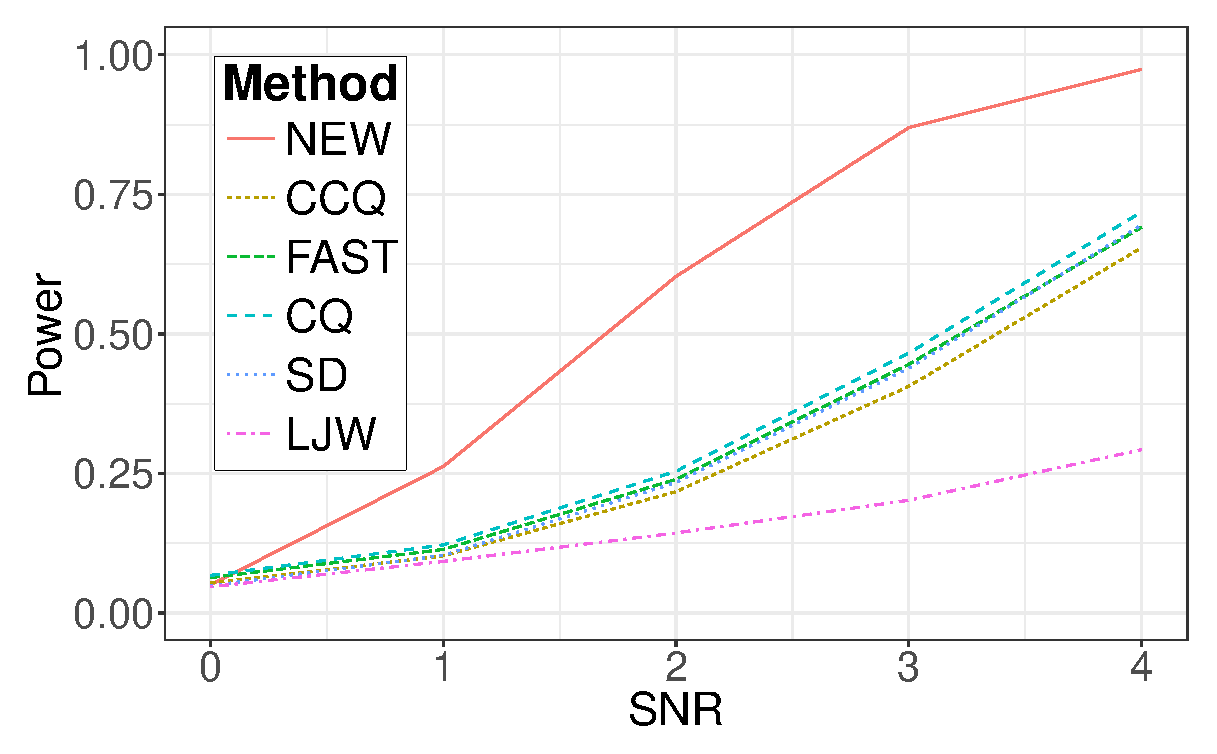
\includegraphics[width=0.3\textwidth]{figure/power/Power1chiSquared05}
    }
    \subfigure[Chi-squared. $\beta=1$.]{
        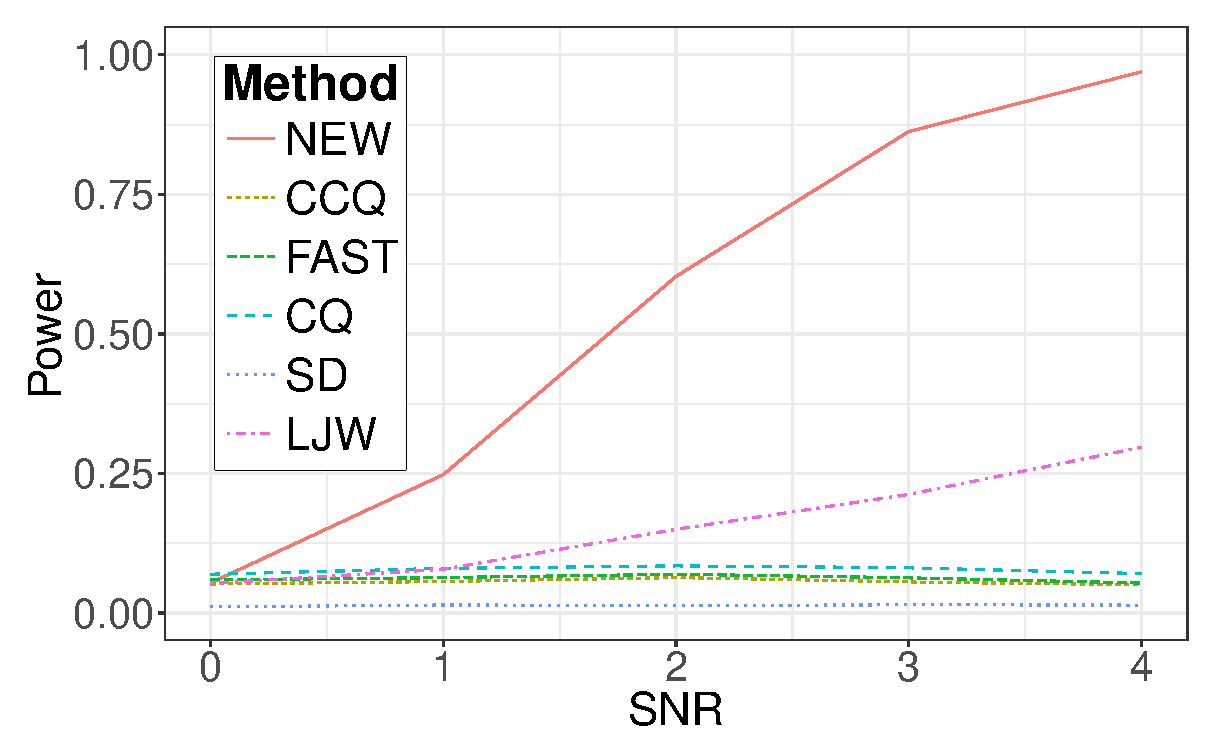
\includegraphics[width=0.3\textwidth]{figure/power/Power1chiSquared1}
    }
    \subfigure[Chi-squared. $\beta=2$.]{
        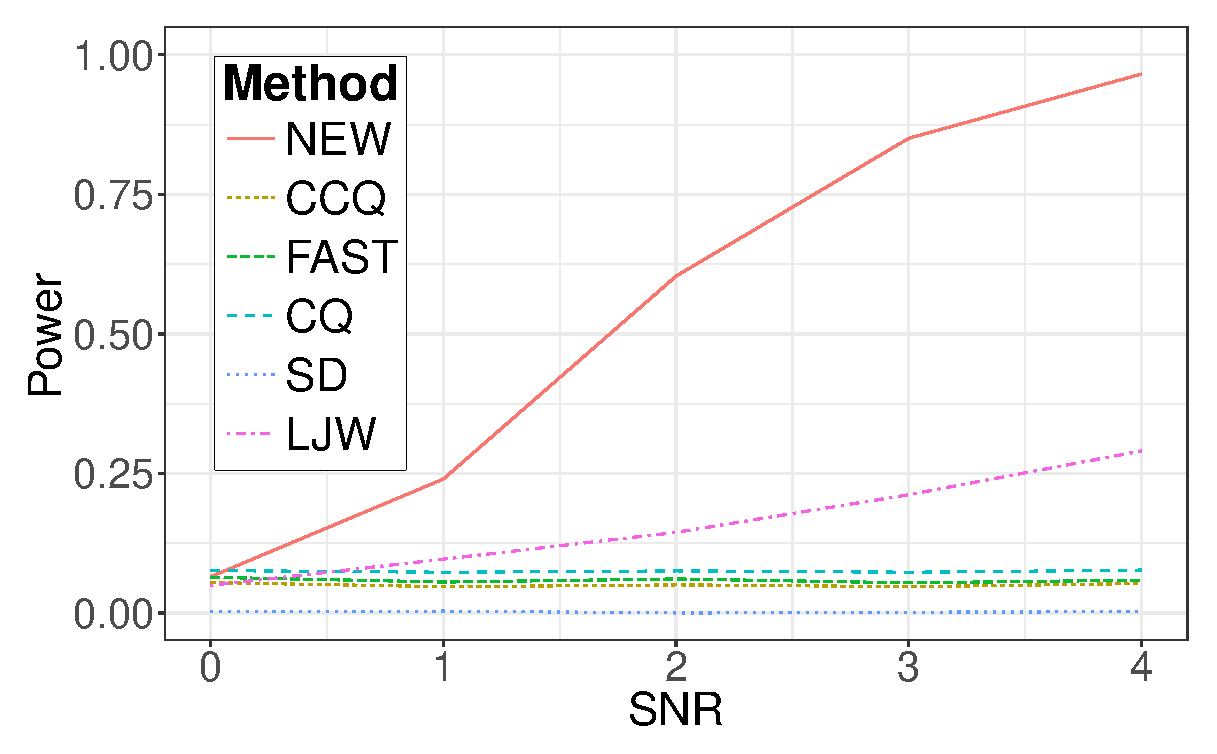
\includegraphics[width=0.3\textwidth]{figure/power/Power1chiSquared2}
    }
    \\
    \subfigure[Student's $t$. $\beta=1/2$.]{
        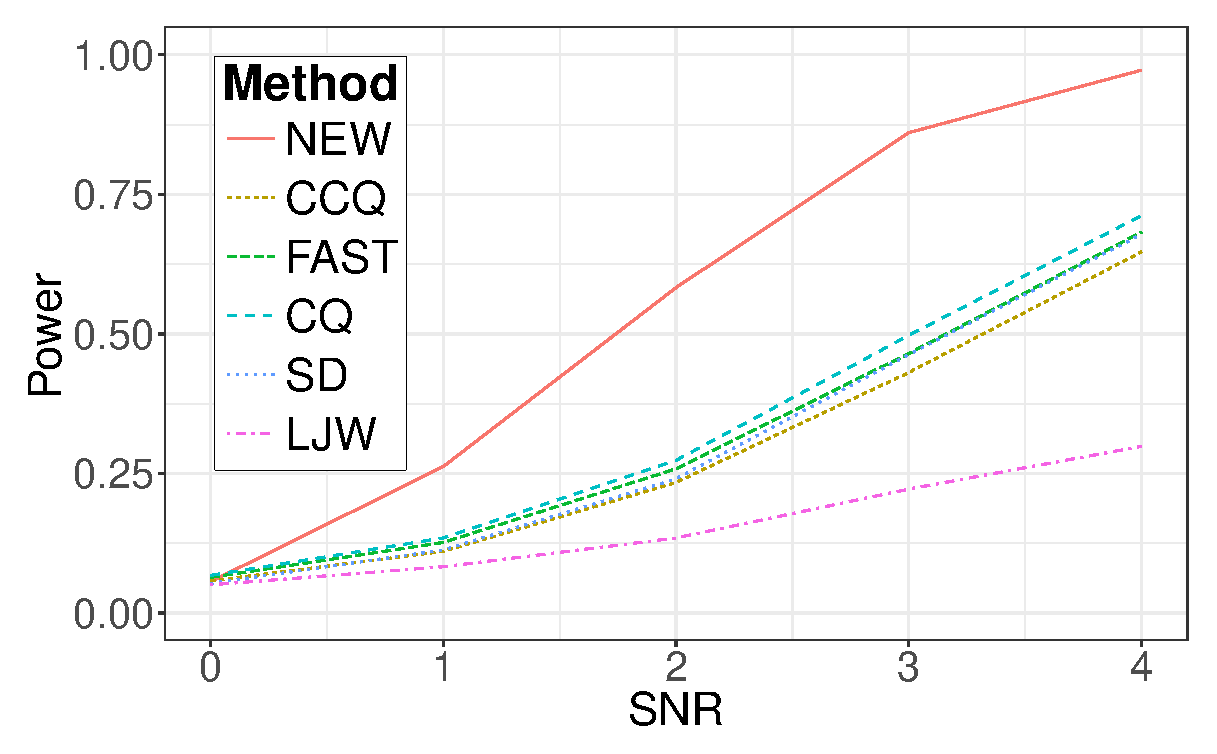
\includegraphics[width=0.3\textwidth]{figure/power/Power1t05}
    }
    \subfigure[Student's $t$. $\beta=1$.]{
        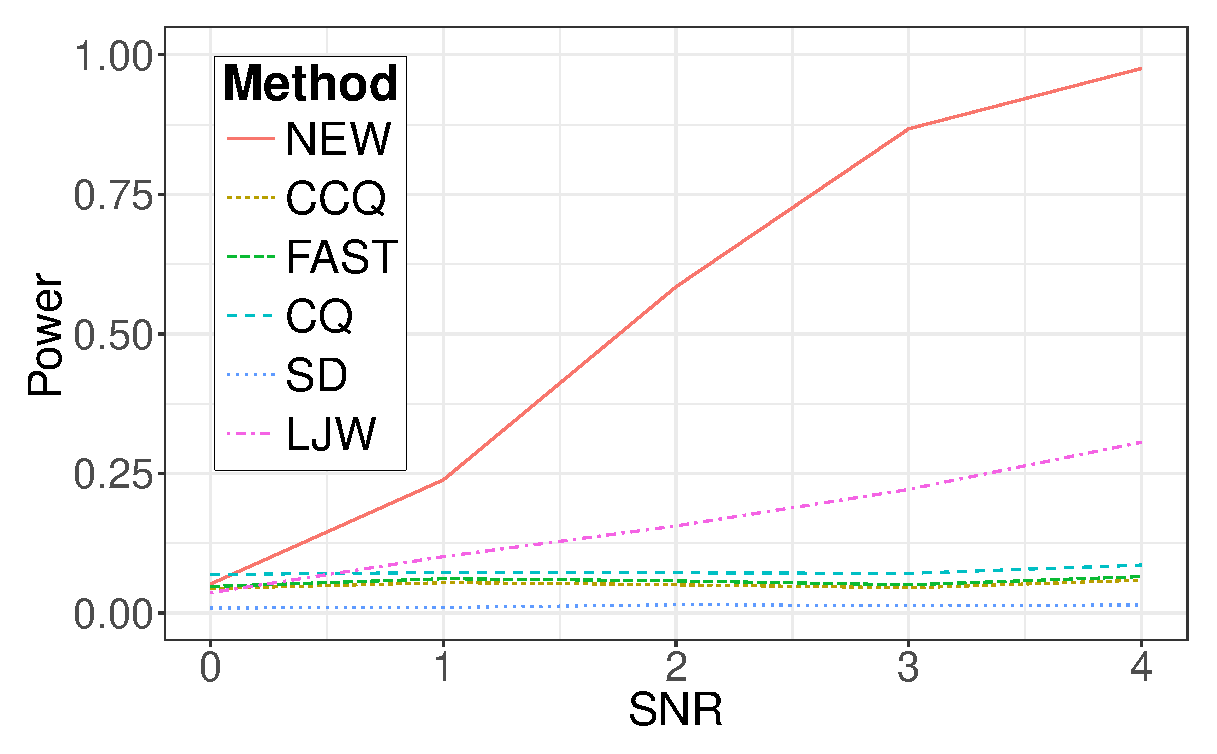
\includegraphics[width=0.3\textwidth]{figure/power/Power1t1}
    }
    \subfigure[Student's $t$. $\beta=2$.]{
        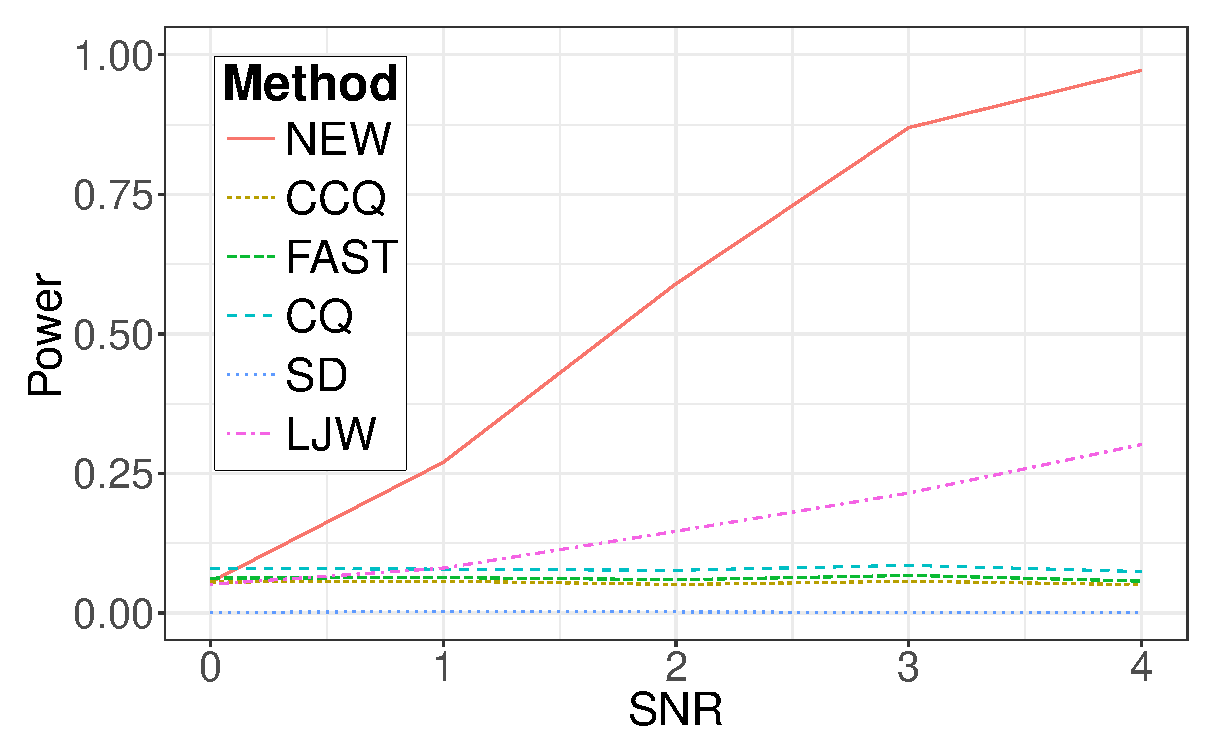
\includegraphics[width=0.3\textwidth]{figure/power/Power1t2}
    }
    \\
    \caption{Empirical power of our test and competing tests. In all cases, $n_1=n_2=100$ and $p=500$.}\label{fig:Power2}
\end{figure}



\subsection{Real data analysis}
In this section, we study the practical problem considered in Ma {\rm et al.}~\cite{Ma2015A}.
The task is to test whether Monday stock returns are equal to those of other trading days on average.
Define an observation to be the log returns of stocks in a day.
Hence $p$ is the total number of stocks.
Let sample $1$ and sample $2$ be the observations on Monday and the other trading days, respectively.
We would like to test $\mathcal{H}_0\, :\mu_1=\mu_2$ vs. $\mathcal{H}_1\,:\mu_1\neq \mu_2$.
We collected the data of $p=710$
 stocks of China
from 01/04/2013 to 12/31/2014. There are total $n_1=95$ Mondays and $n_2=388$ other trading days. 


Using~\eqref{rEstimate} with $R=50$, we have $\hat{r}=1$.
In fact, the first eigenvalue of $\BS$ is $0.14$, which accounts for $\lambda_1(\BS)/\mytr(\BS)=24.86\%$ of the total volatility.
In comparison, the second eigenvalue is only $0.02$.
Hence there's clearly a spiked eigenvalue.
This phenomenon is reasonable since different stock returns are heavily correlated with a common factor, that is the market index; see, e.g.,~\cite{Ma2015A}.
We take $r=1$ and perform the proposed test.
The $p$ value is $0.149$, which is obtained by permutation method with $1000$ permutations.
Hence the null hypothesis can not be rejected for $\alpha=0.05$.
We draw the same conclusion as Ma {\rm et al.}~\cite{Ma2015A}.


\section{Discussion}



This paper is concerned with the problem of testing the equality of means under the spiked covariance model.
We find that Chen and Qin~\cite{Chen2010A}'s test statistic is not asymptotically normal distributed under the spiked covariance model. 
Although a corrected $T_{CQ}$ test can be defined, its power behavior is unsatisfactory.
The recently proposed random projection test procedures suggest that the power of tests may be boosted using the projected data.
By maximizing an average SNR, we find the optimal projection subspace is the orthogonal complement of the principal subspace.
By projecting data onto the (estimated) optimal subspace, we proposed a new test.
The asymptotic normality of the new test statistic is proved and the asymptotic power of the new test is given.
    Theoretical and simulation results show that the new test outperforms the competing tests substantially under the spiked covariance model.


In another paper, Zhao and Xu~\cite{Zhao2016A} proved that their test statistic can be written in the form of projection. Their simulation results showed that their test performs well under strong correlations.
Our work partially explains why their test performs well, although their projection is different from ours. 

 The spiked covariance model is an important correlation pattern and has been widely used in PCA studies.
 In the realm of PCA, authors focus on the principal subspace.
 As our work has shown, however, the complement of the principal subspace may be more useful in hypothesis testing. 


The asymptotic normality of our test statistic relies on the assumption $\sqrt{p}/n\to 0$. In the situation of small $n$ or very large $p$, the critical value of the new test can be determined by permutation method. It remains a theoretical interest to study the asymptotic behavior of permutation based test in these situations.

The normality assumption is very important for this paper.
In particular, our derivations and proofs heavily rely on the fact that $\BS$ is independent of $\bar{X}_1,\bar{X}_2$.
Nevertheless, the simulation results show that the performance of our test is satisfactory under certain non-normal distributions.
It is an interesting but challenging problem to study the robustness of our test and extend the results to other distributions.





\section*{Acknowledgments}
The authors thank the Editor-in-Chief, the Associate Editor and the referees for helpful comments and suggestions that improve the paper considerably.
This work was supported by the National Natural Science Foundation of China under Grant No. 11471035, 11471030.
\begin{appendices}
    \section{Proofs of the results in Section~\ref{sec:chen}}\label{appendixA}
\begin{proof}[\textbf{Proof of Lemma~\ref{quadraticFormCLT}}]
    By a standard orthogonal transformation, we can write
    \begin{equation*}
        \frac{Y_n^\top  \BA_n Y_n-\myE Y_n^\top  \BA_n Y_n}{\{\myVar(Y_n^\top  \BA_n Y_n)\}^{1/2}}=\sum_{i=1}^{k_n}\frac{\lambda_i(\BA_n)}{\{2\mytr(\BA_n^2)\}^{1/2}}(Z_{ni}^2-1),
    \end{equation*}
    where $Z_{n1},\ldots,Z_{n k_n}$ are independent standard normal random variables.

    If~\eqref{quadraticEigen} holds, then
        \begin{align*}
            &\sum_{i=1}^{k_n}\myE\left[\frac{\lambda_i^2(\BA_n)}{2\mathrm{tr}(\BA_n^2)}{(Z_{ni}^2-1)}^2\left\{\frac{\lambda_i^2(\BA_n)}{2\mathrm{tr}(\BA_n^2)}{(Z_{ni}^2-1)}^2\geq \epsilon\right\}\right]\\
            \leq&\sum_{i=1}^{k_n}
            \frac{\lambda_i^2(\BA_n)}{2\mytr(\BA_n^2)}
            \myE\left[{(Z_{n1}^2-1)}^2\left\{\frac{\lambda_{1}(\BA_n^2)}{2\mytr(\BA_n^2)}{(Z_{n1}^2-1)}^2\geq \epsilon\right\}\right]\\
            =&
            \frac{1}{2}\myE\left[{(Z_{n1}^2-1)}^2\left\{\frac{\lambda_{1}(\BA_n^2)}{2\mytr(\BA_n^2)}{(Z_{n1}^2-1)}^2\geq \epsilon\right\}\right]\to 0.
        \end{align*}
    Hence~\eqref{quadratic} follows by Lindeberg's central limit theorem.

    Conversely, if~\eqref{quadratic} holds, we will prove that there is a subsequence of $\{n\}$ along which~\eqref{quadraticEigen} holds. Then~\eqref{quadraticEigen} follows by a standard contradiction argument. 

    Denote $c_{ni}=\lambda_i(\BA_n)/\{2\mytr(\BA_n^2)\}^{1/2}$, $i\in\{1,\ldots,k_n\}$.
    Since~\eqref{quadratic} holds, the characteristic function of
        $
        \sum_{i=1}^{k_n}c_{ni}(Z_{ni}^2-1)
    $
    converges to $\exp(-t^2/2)$ for every $t$.
    Denote by $\ln z$ $(z\in\mathbb{C})$ the principal branch of the complex logarithm.
    For $t\in (-1/2,1/2)$, we have
        \begin{align*}
            &\myE\left[\exp\left\{it \sum_{j=1}^{k_n}c_{nj}(Z_{nj}^2-1)\right\}\right]
            =
            \exp\left\{-i\left(\sum_{j=1}^{k_n}c_{nj}\right)t-
        \frac{1}{2}\sum_{j=1}^{k_n}\ln (1-i2c_{nj}t ) \right\}\\
            =&
            \exp\left\{
            -i\left(\sum_{j=1}^{k_n}c_{nj}\right) t+
            \frac{1}{2}\sum_{j=1}^{k_n}\sum_{\ell=1}^{+\infty}\frac{1}{\ell}(i2c_{nj}t )^\ell
        \right\}
            =
            \exp\left[
            -i\left(\sum_{j=1}^{k_n}c_{nj}\right) t+
        \frac{1}{2}\sum_{\ell=1}^{+\infty}\left\{\sum_{j=1}^{k_n}(c_{nj})^\ell\right\}\frac{1}{\ell}{(i2t)}^\ell\right]\\
            =&
            \exp\left[
            -\frac{1}{2}t^2+
        \frac{1}{2}\sum_{\ell=3}^{+\infty}\left\{\sum_{j=1}^{k_n}{(c_{nj})}^\ell\right\}\frac{1}{\ell}{(i2t)}^\ell \right],
        \end{align*}
    where the second equality holds since $0\leq c_{ni}\leq \sqrt{2}/2$ by definition.
    Let $b_{n\ell}=\sum_{j=1}^{k_n}{(c_{nj})}^\ell$, $n\in\{1,2,\ldots\}$ and $\ell\in\{3,4,\ldots\}$.
    We have
    $$\left|b_{nl}\right|=\left|\sum_{j=1}^{k_n}{(c_{nj})}^\ell\right|\leq \left|\sum_{j=1}^{k_n}{(c_{nj})}^2\right|=\frac{1}{2}.$$
    By Helly's selection theorem, there's a subsequence of $\{n\}$ along which $\lim_{n\to \infty}b_{n\ell}=b_\ell$ exists for every $\ell$.
    For this subsequence, applying the dominated convergence theorem yields
            $$\myE \left[\exp\left\{it \sum_{j=1}^{k_n}c_{nj}(Z_{nj}^2-1)\right\}\right]
            \to
            \exp\left\{
            -\frac{1}{2}t^2+
        \frac{1}{2}\sum_{\ell=3}^{+\infty}b_\ell\frac{1}{\ell}{(i2t)}^\ell\right\},
            \quad t\in\left(-\frac{1}{2},\frac{1}{2}\right).
            $$
            But the left hand side converges to $\exp(-t^2/2)$.
            It follows that
            $$
            -\frac{1}{2}t^2+
            \frac{1}{2}\sum_{\ell=3}^{+\infty}b_\ell\frac{1}{\ell}{(i2t)}^\ell
            =-\frac{1}{2}t^2+ 2\pi m i,
            \quad t\in\left(-\frac{1}{2},\frac{1}{2}\right),
            $$
            for some integer $m$.
            By the uniqueness of power series, we must have $m=0$ and $b_\ell=0$ for $\ell\geq 3$. Then~\eqref{quadraticEigen} follows by noting that $b_{n4}\geq \max_j{(c_{nj})}^4$.
\end{proof}





\begin{proof}[\textbf{Proofs of Theorems~\ref{Chenstheory1} and~\ref{Chenstheory2}}]
    In both Theorems, (a) is a corollary of (b).
    We shall prove (b) of Theorems~\ref{Chenstheory1} and~\ref{Chenstheory2} simultaneously.
    
    Note that $(n_k-1)\BS_k\sim \text{Wishart}_p(n_k-1,\bSigma)$, $k\in \{1,2\}$,
    where $\text{Wishart}_p(m,\Psi)$ is the $p$-dimensional Wishart distribution with parameter $\Psi$ and $m$ degrees of freedom.
    We have 
    $$
 \myE\left(\frac{1}{n_1}\mytr \BS_1+\frac{1}{n_2}\mytr \BS_2\right)=\tau \mytr\bSigma,
    $$
    and
\begin{align*}
    &\myVar\left(\frac{1}{n_1}\mytr \BS_1+\frac{1}{n_2}\mytr \BS_2\right)=
    \left\{\frac{2}{n_1^2(n_1-1)}+\frac{2}{n_2^2(n_2-1)}\right\}\mytr (\bSigma^2)\\
    =&
    O\left\{\frac{1}{n^3}(p^{2\beta}+p)\right\}=O\left(\frac{p^{2\beta}}{n^3}\right).
\end{align*}
    It follows that
\begin{align*}
    &\frac{1}{n_1}\mytr \BS_1+\frac{1}{n_2}\mytr \BS_2=
\tau \mytr \bSigma+O_P\left(\frac{1}{n\sqrt{n}}p^{\beta}\right)\\
    =&\tau \sum_{i=1}^r (\blambda_i+\sigma^2)+\tau(p-r)\sigma^2+O_P\left(\frac{1}{n\sqrt{n}}p^{\beta}\right)\\
    =&\tau p^{\beta} \sum_{i=1}^r \omega_i+\tau(p-r)\sigma^2+o_P\left(\frac{1}{n}p^{\beta}\right).
\end{align*}
Thus,
\begin{equation}\label{eq:kkk1}
\frac{1}{\tau p^\beta}\left(\frac{1}{n_1}\mytr \BS_1+\frac{1}{n_2}\mytr \BS_2\right)
=\sum_{i=1}^r \omega_i+p^{1-\beta}\sigma^2+o_P(1).
\end{equation}

    Next we deal with $\|\bar{X}_1-\bar{X}_2\|^2$.
    Note that we have
    $$
    \|\bar{X}_1-\bar{X}_2\|^2=
    \|\BV^\top (\bar{X}_1-\bar{X}_2)\|^2+
    \|\tilde{\BV}^\top (\bar{X}_1-\bar{X}_2)\|^2.
    $$
    These two terms are independent.
For the first term, note that $\BV^\top (\bar{X}_1-\bar{X}_2)\sim \mathcal{N}_r \{\BV^\top  (\mu_1-\mu_2),\tau (\bLambda+\sigma^2 \BI_r) \}$, we have
\begin{align*}
    \|\BV^\top (\bar{X}_1-\bar{X}_2)\|^2&\overset{d}{=}
    \sum_{i=1}^r \left[\sqrt{\tau (\lambda_i+\sigma^2)}Z_i+\{\BV^\top  (\mu_1-\mu_2)\}_i \right]^2\\
    &=\tau p^{\beta}
    \sum_{i=1}^r
    \left[ \sqrt{p^{-\beta}(\lambda_i+\sigma^2)}Z_i+\frac{1}{\sqrt{\tau p^{\beta}}}\{\BV^\top  (\mu_1-\mu_2)\}_i \right]^2.
\end{align*}
    By the assumptions of the theorem,  we have that
    \begin{equation}\label{eq:kkk2}
        \frac{1}{\tau p^{\beta}}\|\BV^\top (\bar{X}_1-\bar{X}_2)\|^2
        \rightsquigarrow
        \sum_{i=1}^r (\sqrt{\omega_i} Z_i+\zeta_i )^2.
    \end{equation}

    As for $\|\tilde{\BV}^\top (\bar{X}_1-\bar{X}_2)\|^2$, we have that
        \begin{align*}
            &\|\tilde{\BV}^\top (\bar{X}_1-\bar{X}_2)\|^2
            =\|\tilde{\BV}^\top (\mu_1-\mu_2)+\tilde{\BV}^\top \{(\bar{X}_1-\mu_1)-(\bar{X}_2-\mu_2)\}\|^2\\
            =&\|\tilde{\BV}^\top (\mu_1-\mu_2)\|^2+
        \|\tilde{\BV}^\top \{(\bar{X}_1-\mu_1)-(\bar{X}_2-\mu_2)\}\|^2+
        2{(\mu_1-\mu_2)}^\top \tilde{\BV}\tilde{\BV}^\top \{(\bar{X}_1-\mu_1)-(\bar{X}_2-\mu_2)\}.
        \end{align*}
    Since $\tilde{\BV}^\top  (\bar{X}_1-\bar{X}_2)\sim \mathcal{N}_{p-r}\{\tilde{\BV}^\top  (\mu_1-\mu_2),  \sigma^2 \tau \BI_{p-r}\}$, by the central limit theorem, we have
    $$
\frac{
\|\tilde{\BV}^\top \{(\bar{X}_1-\mu_1)-(\bar{X}_2-\mu_2)\}\|^2-\sigma^2 \tau (p-r)}{\sigma^2 \tau\sqrt{2(p-r)}}\rightsquigarrow  \mathcal{N}(0,1).
    $$
    For the intersection term, we have
        \begin{align*}
            &2{(\mu_1-\mu_2)}^\top \tilde{\BV}\tilde{\BV}^\top \{(\bar{X}_1-\mu_1)-(\bar{X}_2-\mu_2)\}
            \sim \mathcal{N}\{0,4\sigma^2 \tau \|\tilde{\BV}^\top (\mu_1-\mu_2)\|^2\}\\
            =& O_P\{\sqrt{\tau}\|\tilde{\BV}^\top (\mu_1-\mu_2)\| \}=o_P(\tau p^{\beta}).
        \end{align*}
    It follows that
    \begin{equation}\label{eq:kkk3}
\frac{1}{\tau p^\beta}
\{\|\tilde{\BV}^\top (\bar{X}_1-\bar{X}_2)\|^2-\sigma^2 \tau (p-r)-\|\tilde{\BV}^\top (\mu_1-\mu_2)\|^2\}
    \rightsquigarrow  
        \sqrt{2}\sigma^2 \delta_{\{{1}/{2}\}}(\beta)Z_0,
    \end{equation}
    where $\delta_{\{{1}/{2}\}}(\beta)$ equals $1$ if $\beta=1/2$ and equals $0$ otherwise.


    Combining~\eqref{eq:kkk1}~\eqref{eq:kkk2} and~\eqref{eq:kkk3} leads to
\begin{align*}
    &\frac{1}{\tau p^{\beta}} T_{CQ}
    =\frac{1}{\tau p^{\beta}}\left(\|\bar{X}_1-\bar{X}_2\|^2-\frac{1}{n_1}\mytr \BS_1-\frac{1}{n_2}\mytr \BS_2\right)\\
    =&
    \frac{1}{\tau p^{\beta}}{\|\BV^\top (\bar{X}_1-\bar{X}_2)\|^2}+
    \frac{1}{\tau p^{\beta}} \{{\|\tilde{\BV}^\top (\bar{X}_1-\bar{X}_2)\|^2-\sigma^2 \tau(p-r)-\|\tilde{\BV}^\top (\mu_1-\mu_2)\|^2}\}\\
    &-\frac{1}{\tau p^{\beta}}\left(\frac{1}{n_1}\mytr \BS_1+\frac{1}{n_2}\mytr \BS_2\right)+\frac{\sigma^2 (p-r)}{p^\beta}+\frac{1}{\tau p^\beta}\|\tilde{\BV}^\top (\mu_1-\mu_2)\|^2\\
    =&
    \sum_{i=1}^r (\sqrt{\omega_i} Z_i+\zeta_i )^2+
\sqrt{2} \sigma^2 \delta_{\{{1}/{2}\}}(\beta)Z_0
    -
    \left(\sum_{i=1}^r \omega_i+p^{1-\beta}\sigma^2\right)
    +\frac{\sigma^2 (p-r)}{p^\beta}+\zeta^*+o_P(1)\\
    \rightsquigarrow &
    \sum_{i=1}^r (\sqrt{\omega_i} Z_i+\zeta_i )^2+
\zeta^*+
\sqrt{2}\sigma^2 \delta_{\{{1}/{2}\}}(\beta)Z_0
    -
    \sum_{i=1}^r \omega_i.
\end{align*}
    This implies the conclusions of Theorem~\ref{Chenstheory1} and Theorem~\ref{Chenstheory2}.


\end{proof}

\begin{proof}[\textbf{Proof of Theorem~\ref{theoremRev}}]
    First we claim that for fixed parameters $\tilde{\blambda}_1,\ldots, \tilde{\blambda}_r$ and $\tilde{\sigma}^2$ satisfying $\tilde{\blambda}_i/\blambda_i\to 1$, $i\in\{1,\ldots,r\}$ and $\tilde{\sigma}^2\to \sigma^2$, we have
    \begin{equation}\label{Reveq1}
        p^{-\beta}F^{-1}(1-\alpha;\tilde{\blambda}_1,\ldots,\tilde{\blambda}_r,\tilde{\sigma}^2)=
        p^{-\beta}F^{-1}(1-\alpha;\blambda_1,\ldots,\blambda_r,\sigma^2)+o(1).
    \end{equation}
    To see this, let $Z_0,\ldots, Z_r$ be iid $\mathcal{N}(0,1)$ random variables, then
    $$
    \tilde{W}\overset{def}{=}\sqrt{2p}\tilde{\sigma}^2 Z_0
+
        \sum_{i=1}^r \tilde{\blambda}_i Z_i^2
            -
        \sum_{i=1}^r \tilde{\blambda}_i\sim F(x;\tilde{\blambda}_1,\ldots,\tilde{\blambda}_r,\tilde{\sigma}^2).
    $$
If $\beta=1/2$, we have
$
    p^{-\beta}\tilde{W}\rightsquigarrow
\sqrt{2}\sigma^2 Z_0 + \sum_{i=1}^r \omega_i Z_i^2 -\sum_{i=1}^r \omega_i
$.
If $\beta>1/2$, we have
$
    p^{-\beta}\tilde{W}\rightsquigarrow
\sum_{i=1}^r \omega_i Z_i^2 -\sum_{i=1}^r \omega_i.
$
    Hence in both cases, the asymptotic distributions of $p^{-\beta}\tilde{W}$ and $p^{-\beta}W$ are both equal to the asymptotic null distribution of $(\tau p^{\beta})^{-1}T_{CQ}$, and the common asymptotic distribution function is continuous.
Note that
$
        p^{-\beta}F^{-1}(1-\alpha;\tilde{\blambda}_1,\ldots,\tilde{\blambda}_r,\tilde{\sigma}^2)
    $
     and
$
        p^{-\beta}F^{-1}(1-\alpha;\blambda_1,\ldots,\blambda_r,\sigma^2)
    $
    are the quantiles of $p^{-\beta}\tilde{W}$ and $p^{-\beta}W$, respectively.
    Hence~\eqref{Reveq1} holds. 
    
    Proposition~\ref{varianceEstimation} asserts that $\hat{\blambda}_i/\blambda_i\xrightarrow{P} 1$, $i\in\{1,\ldots,r\}$ and $\hat{\sigma}_*^2\xrightarrow{P} \sigma^2$.
    Then for every subsequence of $\{n\}$, there is a further subsequence along which $\hat{\blambda}_i/\blambda_i\to 1$, $i\in\{1,\ldots,r\}$ and $\hat{\sigma}_*^2\to \sigma^2$ almost surely.
    Hence along this further subsequence we have
    $$
        p^{-\beta}F^{-1}(1-\alpha;\hat{\blambda}_1,\ldots,\hat{\blambda}_r,\sigma_{*}^2)=
        p^{-\beta}F^{-1}(1-\alpha;\blambda_1,\ldots,\blambda_r,\sigma^2)+o(1)
    $$
    almost surely.
    That is to say
    $$
        p^{-\beta}F^{-1}(1-\alpha;\hat{\blambda}_1,\ldots,\hat{\blambda}_r,\sigma_{*}^2)=
        p^{-\beta}F^{-1}(1-\alpha;\blambda_1,\ldots,\blambda_r,\sigma^2)+o_P(1).
    $$
    Thus,
\begin{align*}
    &\Pr\{\tau^{-1}T_{CQ} > F^{-1}(1-\alpha;\hat{\blambda}_1,\ldots,\hat{\blambda}_r,\hat{\sigma}_*^2)\}
    \\
    =&
    \Pr\{(\tau p^{\beta})^{-1}T_{CQ} +o_P(1) > p^{-\beta}F^{-1}(1-\alpha;\blambda_1,\ldots,\blambda_r,\sigma^2)\}
    \\
    =& \alpha +o(1),
\end{align*}
    where the last equality follows from Slutsky's theorem.
    This completes the proof.
\end{proof}




\section{Proofs of the results in Section~\ref{methodology}}\label{appendixB}

\begin{lemma}[Weyl's inequality]
Let $\BA$ and $\BB$ be two symmetric $n\times n$ matrices and $\BC=\BA+\BB$. If $r+s-1 \leq  i\leq j+k-n$, we have
\begin{equation*}
\lambda_j(\BA)+\lambda_k(\BB)\leq \lambda_i(\BC) \leq \lambda_r(\BA)+\lambda_s(\BB).
\end{equation*}
    (See, e.g., Theorem $4.3.1$ of ~\cite{Horn1985Matrix}.)
\end{lemma}

\begin{lemma}[\cite{Cai2015Optimal}, Proposition 1]\label{pert}
    Let $\BA_1$ and $\BA_2$ be $p\times p$ symmetric matrices. Let $r<p$ be arbitrary and let $\BV_1, \BV_2\in \mathbb{O}_{p,r}$ be formed by the $r$ leading singular vectors of $\BA_1$ and $\BA_2$, respectively.
    Then
    $$
    \|\BA_1-\BA_2\|\geq \frac{1}{2}\{\lambda_r(\BA_2)-\lambda_{r+1}(\BA_2)\}\|\BV_1 \BV_1^\top - \BV_2 \BV_2^\top \|.
    $$
\end{lemma}


\begin{lemma}[\cite{DAVIDSON2001317}, Theorem II.7]\label{DSbound}
    Let $\BZ$ be a $p\times n$ random matrix with iid $\mathcal{N}(0,1)$ entries.
    Then for any $t>0$,
    \begin{align*}
        &\Pr\left\{\sqrt{\lambda_1(\BZ \BZ^\top  )}>\sqrt{n}+\sqrt{p}+t\right\}\leq e^{-t^2/2},
        \\
        &\Pr\left\{\sqrt{\lambda_{\min(n,p)}(\BZ \BZ^\top  )}<\sqrt{n}-\sqrt{p}-t \right\}\leq e^{-t^2/2}.
    \end{align*}
\end{lemma}
    The following corollary of Lemma~\ref{DSbound} is useful.

\begin{corollary}\label{corNorm}
Suppose that $\BW_n$ is a $p \times p$ random matrix which is distributed as $\mathrm{Wishart}_p(n,\BI_{p})$.
    Then as $n,p\to \infty$,
$$
\left\|\frac{1}{n}\BW_n-\BI_p\right\|=O_P\left\{\max\left(\sqrt{\frac{p}{n}},\frac{p}{n}\right)\right\}.
$$
\end{corollary}
\begin{proof}
    Since the eigenvalues of $n^{-1}\BW_n-\BI_p$ are $n^{-1}\lambda_1(\BW_n)-1,\ldots, n^{-1}\lambda_p(\BW_n)-1$, we have
    $$\left\|\frac{1}{n}\BW_n-\BI_p\right\|=\max\left\{\frac{1}{n}\lambda_1(\BW_n)-1,1-\frac{1}{n}\lambda_p(\BW_n)\right\}.$$
This, together with the union bound, yields
$$
\Pr\left\{\left\|\frac{1}{n}\BW_n-\BI_p\right\|>4\left(\sqrt{\frac{p}{n}}+\frac{p}{n}\right)\right\}
    \leq
    \Pr\{\lambda_1(\BW_n)>(\sqrt{n}+2\sqrt{p})^2\}+
    \Pr\{\lambda_p(\BW_n)<n-4\sqrt{np}-4p\}.
$$
    For the first term, we have    
    $$
    \Pr\{\lambda_1(\BW_n)>(\sqrt{n}+2\sqrt{p})^2\}=
    \Pr\left\{\sqrt{\lambda_1(\BW_n)}>\sqrt{n}+2\sqrt{p}\right\}\leq e^{-p/2},
    $$
 where the last inequality follows from Lemma~\ref{DSbound} with $t=\sqrt{p}$.

    We now show that the second term is also bounded by $e^{-p/2}$.
    To see this, note that if $p>n/4$, then $n-4\sqrt{np}-4p\leq n-4p<0$.
    In this case, $\Pr\{\lambda_p(\BW_n)<n-4\sqrt{np}-4p\}=0$.
    If $p\leq n/4$, we have
    \begin{align*}
        &\Pr\{\lambda_p(\BW_n)<n-4\sqrt{np}-4p\}
    \leq
    \Pr\{\lambda_p(\BW_n)<n-4\sqrt{np}+4p\}\\
        =&
        \Pr\left\{\sqrt{\lambda_p(\BW_n)}<\sqrt{n}-2\sqrt{p}\right\}
        \leq e^{-p/2},
    \end{align*}
    where the last inequality follows from Lemma~\ref{DSbound} with $t=\sqrt{p}$.

    Now we conclude that
    $$
    \Pr\left\{\left\|\frac{1}{n}\BW_n-\BI_p\right\|>4\left(\sqrt{\frac{p}{n}}+\frac{p}{n}\right)\right\}
    \leq 2 e^{-p/2}.
    $$
    Consequently,
    $$\left\|\frac{1}{n}\BW_n-\BI_p\right\|=O_P\left(\sqrt{\frac{p}{n}}+\frac{p}{n}\right)=O_P\left\{\max\left(\sqrt{\frac{p}{n}},\frac{p}{n}\right)\right\}.$$
\end{proof}



\begin{lemma}\label{eigenconsisLemma}
    Under Assumption~\ref{theModel}, we have, for each $i\in\{1,\ldots,r\}$,
    \begin{equation}\label{eigenconsisResult1}
        \lambda_i(\BS)= \blambda_i+\frac{p+n-r}{n}\sigma^2+
        O_P\left\{\max\left(\frac{p^{\beta}}{\sqrt{n}},1\right)\right\},
    \end{equation}
    and
    \begin{equation}\label{eigenconsisResult2}
        \hat{\sigma}^2=
\left(1-\frac{r}{n}\right)\sigma^2+
O_P\left\{\max\left(\frac{1}{\sqrt{np}},\frac{1}{p}\right)\right\}.
    \end{equation}
\end{lemma}
\begin{proof}[\textbf{Proof}]
    Let $\bSigma=\BU\BE\BU^\top $ denote the spectral decomposition of $\bSigma$, where
     $\BU=(\BV,\tilde{\BV})$ and $\BE=\mydiag(\blambda_1+\sigma^2,\ldots,\blambda_r+\sigma^2,\sigma^2,\ldots,\sigma^2)$.
    Let $\bZ$ be a $p\times n$ random matrix with iid $\mathcal{N}(0,1)$ entries.
Denote $\bZ={(\bZ_{(1)}^\top ,\bZ_{(2)}^\top )}^\top $, where $\bZ_{(1)}$ and $\bZ_{(2)}$ are the first $r$ rows and last $p-r$ rows of $\bZ$. 
Then the sample covariance matrix $\BS$ has the same distribution as the random matrix
$
    n^{-1} \BU \BE^{1/2} \bZ \bZ^\top  \BE^{1/2} \BU^\top 
$.
So we have $\lambda_i(\BS)\overset{d}{=} n^{-1}\lambda_i(\bZ^\top  \BE \bZ)$, $i\in\{1,\ldots,r\}$, and $\mytr(\BS)\overset{d}{=} n^{-1}\mytr(\BZ^\top  \BE \BZ)$.

To prove~\eqref{eigenconsisResult1}, we only need to consider $n^{-1}\lambda_i(\bZ^\top  \BE \bZ)$, $i\in\{1,\ldots, r\}$.
Note that
$
    \bZ^\top  \BE \bZ= \bZ_{(1)}^\top  (\bLambda +\sigma^2 \BI_r) \bZ_{(1)}+
\sigma^2 \bZ_{(2)}^\top   \bZ_{(2)}
$.
From this and Weyl's inequality, 
for $i\in\{1,\ldots, r\}$, we have 
\begin{align*}
    &\left|\frac{1}{n}\lambda_i(\BZ^\top  \BE \BZ)
    -\frac{1}{n}\lambda_i\{\BZ_{(1)}^\top  (\bLambda+\sigma^2 \BI_r)\BZ_{(1)}\}
-\frac{p-r}{n}\sigma^2
\right|
    \\
    =&\left|\lambda_i\left(\frac{1}{n}\BZ^\top  \BE \BZ\right)
    -\lambda_i\left\{\frac{1}{n}\BZ_{(1)}^\top  (\bLambda+\sigma^2 \BI_r)\BZ_{(1)}+\frac{p-r}{n}\sigma^2 \BI_{n}\right\}
\right|
    \\
    \leq &
    \left\|\frac{1}{n}\BZ^\top  \BE \BZ
-\frac{1}{n}\BZ_{(1)}^\top  (\bLambda+\sigma^2 \BI_r)\BZ_{(1)}
    -\frac{p-r}{n}\sigma^2\BI_{n}
    \right\|
    \\
    = &
    \left\|
    \frac{1}{n}\sigma^2 \bZ_{(2)}^\top   \bZ_{(2)}
    -\frac{p-r}{n}\sigma^2\BI_{n}
    \right\|
    \\
    = &
    \frac{p-r}{n}
\sigma^2
    \left\|
    \frac{1}{p-r}
     \bZ_{(2)}^\top   \bZ_{(2)}
    -\BI_{n}
    \right\|.
\end{align*}
    But Corollary~\ref{corNorm} implies that
    $$
        \left\|
        \frac{1}{p-r}
         \bZ_{(2)}^\top   \bZ_{(2)}
        -\BI_{n}
        \right\|=O_P\left\{\max\left(\sqrt{\frac{n}{p-r}},\frac{n}{p-r}\right)\right\}.
    $$
Thus, for $i\in\{1,\ldots,r\}$,
\begin{equation}\label{toutengjiayou1}
\frac{1}{n}\lambda_i(\BZ^\top  \BE \BZ)
=\frac{1}{n}\lambda_i\{\BZ_{(1)}^\top  (\bLambda+\sigma^2 \BI_r)\BZ_{(1)}\}
+\frac{p-r}{n}\sigma^2
+
O_P\left\{\max\left(\sqrt{\frac{p}{n}},1\right)\right\}.
\end{equation}
Next we deal with $n^{-1}\lambda_i\{\BZ_{(1)}^\top  (\bLambda+\sigma^2 \BI_r)\BZ_{(1)}\}$.
For $i\in\{1,\ldots, r\}$, we have
    \begin{align*}
        &\left|\frac{1}{n}\lambda_i \{\bZ_{(1)}^\top (\bLambda+\sigma^2 \BI_r)\bZ_{(1)}\}-(\blambda_i +\sigma^2)\right|\\
        =&
        \left|\lambda_i \left\{\frac{1}{n}(\bLambda+\sigma^2 \BI_r)^{1/2}\bZ_{(1)}\bZ_{(1)}^\top (\bLambda+\sigma^2 \BI_r)^{1/2}\right\}
        -\lambda_i(\bLambda+\sigma^2 \BI_r)\right|\\
        \leq &
        \left\|
        \frac{1}{n}(\bLambda+\sigma^2 \BI_r)^{1/2}\bZ_{(1)}\bZ_{(1)}^\top (\bLambda+\sigma^2 \BI_r)^{1/2}
        -(\bLambda+\sigma^2 \BI_r)
        \right\|\\
        = &
        \left\|
        (\bLambda+\sigma^2 \BI_r)^{1/2}\left(\frac{1}{n}\bZ_{(1)}\bZ_{(1)}^\top -\BI_r\right)(\bLambda+\sigma^2 \BI_r)^{1/2}
        \right\|\\
        \leq &
        (\blambda_1 + \sigma^2)
        \left\|\frac{1}{n}\bZ_{(1)}\bZ_{(1)}^\top -\BI_r\right\|\\
        = &
        O_P\left(\frac{\blambda_1}{\sqrt{n}}\right),
    \end{align*}
    where the first inequality follows from Weyl's inequality and the last equality follows from Corollary~\ref{corNorm}.
    This, together with~\eqref{toutengjiayou1}, leads to
$$
\frac{1}{n}\lambda_i(\BZ^\top  \BE \BZ)=
\blambda_i+\frac{p+n-r}{n}\sigma^2+O_P\left\{\max\left(\sqrt{\frac{p}{n}},\frac{\blambda_1}{\sqrt{n}},1\right)\right\},
$$
where $i\in\{1,\ldots, r\}$.
Then~\eqref{eigenconsisResult1} follows from $\blambda_1\asymp p^{\beta}$ and $\beta\geq 1/2$.
    
    Now we prove~\eqref{eigenconsisResult2}.
    We note that
    $$
\hat{\sigma}^2=\frac{1}{p-r}\left\{\mytr(\BS)-\sum_{i=1}^r \lambda_i(\BS)\right\}
    \overset{d}{=}
    \frac{1}{n(p-r)}\left\{\mytr(\BZ^\top  \BE \BZ)-\sum_{i=1}^r \lambda_i(\BZ^\top  \BE \BZ)\right\}.
    $$
    For the term $\mytr(\BZ^\top  \BE \BZ)$, we have
    $
    \mytr(\bZ^\top  \BE \bZ)= \mytr\{\bZ_{(1)}^\top  (\bLambda +\sigma^2 \BI_r) \bZ_{(1)}\}+
       \sigma^2 \mytr( \bZ_{(2)}^\top   \bZ_{(2)})
    $.
    Since $\mytr( \bZ_{(2)}^\top   \bZ_{(2)})\sim \chi^2\{ n(p-r)\}$, by the central limit theorem, we have
    $$\mytr( \bZ_{(2)}^\top   \bZ_{(2)})=n(p-r)+O_P(\sqrt{np}).$$
    It follows that
    \begin{equation}\label{toutengjiayou2}
        \mytr(\bZ^\top  \BE \bZ)= \mytr\{\bZ_{(1)}^\top  (\bLambda +\sigma^2 \BI_r) \bZ_{(1)}\}+
            n(p-r)\sigma^2+O_P(\sqrt{np}).
    \end{equation}
    In view of~\eqref{toutengjiayou1}, we have
    $$
\sum_{i=1}^r\lambda_i(\BZ^\top  \BE \BZ)
=\mytr\{\BZ_{(1)}^\top  (\bLambda+\sigma^2 \BI_r)\BZ_{(1)}\}
+r(p-r)\sigma^2
+
O_P\{\max(\sqrt{np},n)\}.
    $$
    This, together with~\eqref{toutengjiayou2}, yields
    $$
    \frac{1}{n(p-r)}\left\{\mytr(\BZ^\top  \BE \BZ)-\sum_{i=1}^r \lambda_i(\BZ^\top  \BE \BZ)\right\}=
\left(1-\frac{r}{n}\right)\sigma^2+
O_P\left\{\max\left(\frac{1}{\sqrt{np}},\frac{1}{p}\right)\right\}.
    $$
\end{proof}

\begin{lemma}\label{conRateLemma}
    Under Assumption~\ref{theModel}, we have
\begin{equation*}
\|\hat{\BV}\hat{\BV}^\top -\BV\BV^\top \|^2 =O_P\left(\frac{p}{p^{\beta}n}\right).
\end{equation*}
\end{lemma}
\begin{remark}
    Theorem 5 of~\cite{Cai2012Sparse} asserts that under certain conditions,
$$
\myE \|\hat{\BV}\hat{\BV}^\top -\BV\BV^\top \|_F^2 =O\left(\frac{p}{p^{\beta}n}\right),
    $$
    where $\|\cdot\|_F$ is the Frobenius norm.
    Moreover, they proved that the convergence rate $p/(p^{\beta}n)$ is in fact minimax optimal.
    However,  Theorem 5 of \cite{Cai2012Sparse} needs the condition $\ln p=O(n)$ which is unwanted.
    This condition is used to control the expectation and hence can be dropped in Lemma~\ref{conRateLemma}.
\end{remark}
\begin{proof}[\textbf{Proof}]
    Since $\|\hat{\BV}\hat{\BV}^\top-\BV\BV^\top\|^2\leq 1$, the conclusion is trivial when $p/(p^{\beta} n)$ is unbounded.
    So without loss of generality, we assume $p/(p^{\beta} n)=O(1)$.
    Define $\BU$, $\BE$, $\bZ$, $\bZ_{(1)}$ and $\bZ_{(2)}$ as in the proof of Lemma~\ref{eigenconsisLemma}.
Without loss of generality, we assume that $\BS= n^{-1}\BU\BE^{1/2}\bZ \bZ^\top \BE^{1/2} \BU^\top$. 
    Similar to the proof of Theorem 5 of~\cite{Cai2012Sparse},
we define 
    $$
    \BS_0=
        \frac{1}{n}\BV(\bLambda+\sigma^2\BI_r)^{1/2}\bZ_{(1)} \bZ_{(1)}^\top(\bLambda+\sigma^2\BI_r)^{1/2}\BV^\top
        +\sigma^2\tilde{\BV}\tilde{\BV}^\top.
    $$
    It can be seen that the set of eigenvalues of $\BS_0$ is the union of the nonzero eigenvalues of the matrix $n^{-1}\BV(\bLambda+\sigma^2\BI_r)^{1/2}\bZ_{(1)} \bZ_{(1)}^\top(\bLambda+\sigma^2\BI_r)^{1/2}\BV^\top$ and $\sigma^2\tilde{\BV}\tilde{\BV}^\top$.
All the nonzero eigenvalues of $\sigma^2\tilde{\BV}\tilde{\BV}^\top$ are $\sigma^2$.
We note that with probability $1$, the first matrix is of rank $r$.
        Define the event
        $$
        A=
        \left\{
            \frac{1}{n}\lambda_r\{\BV(\bLambda+\sigma^2 \BI_r)^{1/2}\bZ_{(1)} \bZ_{(1)}^\top(\bLambda+\sigma^2 \BI_r)^{1/2}\BV^\top\}
        >\sigma^2
        \right\}.
        $$
        On the event $A$, the eigenspace of $\BS_0$ associated with the $r$ leading eigenvalues is exactly $\BV \BV^\top$, although the individual columns of $\BV$ need not be the leading eigenvectors of $\BS_0$.
    Applying Lemma~\ref{pert} to $\BS$ and $\BS_0$ yields
    \begin{equation}\label{toutengjiayou3}
    \|\hat{\BV}\hat{\BV}^\top - \BV\BV ^\top\| \mathbf{1}_{\{A\}}\leq
        \frac{2}{\lambda_r(\BS_0)-\lambda_{r+1}(\BS_0)}\|\BS-\BS_0\|\mathbf{1}_{\{A\}}.
    \end{equation}
    Note that
$$
\lambda_r\left\{\frac{1}{n}\BV(\bLambda+\sigma^2\BI_r)^{1/2}\bZ_{(1)} \bZ_{(1)}^\top(\bLambda+\sigma^2\BI_r)^{1/2}\BV^\top\right\}
    =
    \frac{1}{n}\lambda_r\{(\bLambda+\sigma^2\BI_r)^{1/2}\bZ_{(1)} \bZ_{(1)}^\top(\bLambda+\sigma^2\BI_r)^{1/2}\}.
$$
By Weyl's inequality,
\begin{align*}
    &\left|
    \frac{1}{n}\lambda_r\{(\bLambda+\sigma^2 \BI_r)^{1/2}\bZ_{(1)} \bZ_{(1)}^\top(\bLambda+\sigma^2 \BI_r)^{1/2}\}
-
    (\blambda_r+\sigma^2)
\right|\\
    =&\left|
\frac{1}{n}\lambda_r\{(\bLambda+\sigma^2 \BI_r)^{1/2}\bZ_{(1)} \bZ_{(1)}^\top(\bLambda+\sigma^2 \BI_r)^{1/2}\}
-
\lambda_r(\bLambda+\sigma^2\BI_r)
\right|
    \\
    \leq&
    \left\|(\bLambda+\sigma^2\BI_r)^{1/2}\left(\frac{1}{n}\bZ_{(1)} \bZ_{(1)}^\top-\BI_r\right)(\bLambda+\sigma^2\BI_r)^{1/2}\right\|\\
    \leq& (\blambda_1+\sigma^2)\left\|\frac{1}{n}\bZ_{(1)} \bZ_{(1)}^\top-\BI_r\right\|
    \\
    =& O_P\left(\frac{\blambda_1+\sigma^2}{\sqrt{n}}\right),
\end{align*}
    where the last equality follows from Corollary~\ref{corNorm}.
    Hence
$$
\frac{1}{n}\lambda_r\{\BV(\bLambda+\sigma^2 \BI_r)^{1/2}\bZ_{(1)} \bZ_{(1)}^\top(\bLambda+\sigma^2 \BI_r)^{1/2}\BV^\top\}
=(\blambda_1+\sigma^2)\left\{1+O_P\left(\frac{1}{\sqrt{n}}\right)\right\}.
        $$
        It follows that $P(A)\to 1$.
        In view of~\eqref{toutengjiayou3}, it is sufficient to show that
        $$
        \frac{2}{\lambda_r(\BS_0)-\lambda_{r+1}(\BS_0)}\|\BS-\BS_0\|\mathbf{1}_{\{A\}}=O_P\left(\sqrt{\frac{p}{p^{\beta}n }}\right).
        $$
        Note that on event $A$, $\lambda_{r+1}(\BS_0)=\sigma^2$ and
        $$\lambda_r(\BS_0)=\frac{1}{n}\lambda_r\{\BV(\bLambda+\sigma^2 \BI_r)^{1/2}\bZ_{(1)} \bZ_{(1)}^\top (\bLambda+\sigma^2 \BI_r)^{1/2}\BV^\top \}.$$
        Hence
\begin{align*}
    &\frac{2}{\lambda_r(\BS_0)-\lambda_{r+1}(\BS_0)}\mathbf{1}_{\{A\}}
    =
    \frac{2}{
    \frac{1}{n}\lambda_r\{\BV(\bLambda+\sigma^2 \BI_r)^{1/2}\bZ_{(1)} \bZ_{(1)}^\top (\bLambda+\sigma^2 \BI_r)^{1/2}\BV^\top \}-\sigma^2}\mathbf{1}_{\{A\}}\\
    =&\frac{2}{\blambda_r\left\{1+O_P\left(\frac{1}{\sqrt{n}}\right)\right\}}\mathbf{1}_{\{A\}}
    =\frac{2}{\blambda_r}\{1+o_P(1)\}.
\end{align*}
    Next we bound $\|\BS-\BS_0\|$. 
    We have
    \begin{align*}
        &\|\BS-\BS_0\|=
        \|(\BV\BV^\top +\tilde{\BV}\tilde{\BV}^\top )(\BS-\BS_0)(\BV\BV^\top +\tilde{\BV}\tilde{\BV}^\top )\|\\
        \leq& \|\BV\BV^\top  (\BS-\BS_0) \BV\BV^\top \|+2 \|\BV\BV^\top  (\BS-\BS_0) \tilde{\BV}\tilde{\BV}^\top \|+\|\tilde{\BV}\tilde{\BV}^\top  (\BS-\BS_0) \tilde{\BV}\tilde{\BV}^\top \|\\
        \leq& \|\BV^\top  (\BS-\BS_0) \BV\|+2 \|\BV^\top  (\BS-\BS_0) \tilde{\BV}\|+\|\tilde{\BV}^\top  (\BS-\BS_0) \tilde{\BV}\|\\
        = &
        2\left\|\frac{\sigma}{n}(\bLambda+\sigma^2 \BI_r)^{1/2}\bZ_{(1)} \bZ_{(2)}^\top \right\|+
        \sigma^2\left\|\frac{1}{n}\bZ_{(2)} \bZ_{(2)}^\top - \BI_{p-r}\right\|\\
        \leq & \frac{2\sqrt{(\lambda_1+\sigma^2)\sigma^2}}{n}\|\bZ_{(1)}\bZ_{(2)}^\top \|+
        \sigma^2\left\|\frac{1}{n}\bZ_{(2)} \bZ_{(2)}^\top - \BI_{p-r}\right\|.
    \end{align*}
    By Corollary~\ref{corNorm}, we have $\|n^{-1}\bZ_{(2)} \bZ_{(2)}^\top - \BI_{p-r}\|=O_p\{\max(\sqrt{p/n},p/n)\}$.
    By the independence of $\bZ_{(1)}$ and $\bZ_{(2)}$, we have
\begin{align*}
    &\myE \|\bZ_{(1)}\bZ_{(2)}^\top \|^2\leq
\myE \|\bZ_{(1)}\bZ_{(2)}^\top \|_F^2
=
\myE \{ \mytr(\bZ_{(1)}\bZ_{(2)}^\top \bZ_{(2)}\bZ_{(1)}^\top ) \}\\
    =&
    \myE\myE \{ \mytr(\bZ_{(1)}\bZ_{(2)}^\top \bZ_{(2)}\bZ_{(1)}^\top )|\BZ_{(1)} \}
    =(p-r)
\myE \{ \mytr(\bZ_{(1)}\bZ_{(1)}^\top ) \}
    =rn(p-r).
\end{align*}
    Hence $\|\bZ_{(1)}\bZ_{(2)}^\top \|=O_P(\sqrt{np})$.
    Combining these bounds leads to
    $$
    \|\BS-\BS_0\|=
O_P\left(\sqrt{\frac{\lambda_1 p}{n}}\right)+O_P\left\{\max\left(\sqrt{\frac{p}{n}},\frac{p}{n}\right)\right\}
    =
    O_P\left(\sqrt{\frac{ p^{\beta}p}{n}}\right)+O_P\left(\frac{p}{n}\right).
    $$
    Thus,
    $$
   \frac{2}{\lambda_r(\BS_0)-\lambda_{r+1}(\BS_0)}\left\|\BS-\BS_0\right\|=
    O_P\left(\sqrt{\frac{p}{p^{\beta}n}}\right)+O_P\left(\frac{p}{p^{\beta}n}\right)=
O_P\left(\sqrt{\frac{p}{p^{\beta}n}}\right),
    $$
    where the last equality holds since we have assumed $p/(p^{\beta}n)=O(1)$.
    This completes the proof.

\end{proof}


\begin{proof}[\textbf{Proof of Proposition~\ref{oracleTheorem}}]
    Note that, for $k\in\{1,2\}$,
    $$
    \frac{n_k-1}{\sigma^2} \mytr(\tilde{\BV}^\top  \BS_k \tilde{\BV})\sim \chi^2\{(p-r)(n_k-1)\}.
    $$
    It follows from the central limit theorem that, for $k\in\{1,2\}$,
    \begin{equation*}
        \frac{1}{\sigma^2}\sqrt{\frac{n_k-1}{2(p-r)}}\{ \mytr(\tilde{\BV}^\top  \BS_k \tilde{\BV})-(p-r)\sigma^2\}\rightsquigarrow \mathcal{N}(0,1).
    \end{equation*}
    Then for $k\in\{1,2\}$, we have
    $$
           \frac{1}{n_k} \mytr(\tilde{\BV}^\top  \BS_k \tilde{\BV}) =
            \frac{p-r}{n_k}\sigma^2 + O_P\left(\frac{\sqrt{p}}{n\sqrt{n}}\right).
    $$
    Thus,
    \begin{equation*}
            T_1-\|\tilde{\BV}^\top (\mu_1-\mu_2)\|^2=
            \|\tilde{\BV}^\top (\bar{X}_1-\bar{X}_2)\|^2-
            \|\tilde{\BV}^\top (\mu_1-\mu_2)\|^2
            -  \tau (p-r)\sigma^2 + O_P\left(\frac{\sqrt{p}}{n\sqrt{n}}\right)
            =
            T_1^{(1)}+T_1^{(2)}
            + O_P\left(\frac{\sqrt{p}}{n\sqrt{n}}\right)
            ,
    \end{equation*}
    where
    \begin{align*}
        T_1^{(1)}&=\|\tilde{\BV}^\top \{(\bar{X}_1-\mu_1)-(\bar{X}_2-\mu_2)\}\|^2   -  \tau (p-r)\sigma^2, \\
        T_1^{(2)}&=2{(\mu_1-\mu_2)}^\top \tilde{\BV}\tilde{\BV}^\top \{(\bar{X}_1-\mu_1)-(\bar{X}_2-\mu_2) \}.
    \end{align*}

It follows from the fact
$\|\tilde{\BV}^\top  \{ (\bar{X}_1-\mu_1)-(\bar{X}_2-\mu_2) \}\|^2\sim \sigma^2\tau\chi^2(p-r)$ that
$$
            \frac{T_1^{(1)}}{\sqrt{2\tau^2 (p-r)\sigma^4}}\sim \frac{\chi^2 (p-r)- (p-r)}{\sqrt{2(p-r)}}.
    $$
    For $T_1^{(2)}$, we have
    \begin{equation*}
            \frac{T_1^{(2)}}{\sqrt{4\tau \|\tilde{\BV}^\top (\mu_1-\mu_2)\|^2\sigma^2}}
            \sim \mathcal{N}(0,1).
    \end{equation*}

    Thus, if $\|\tilde{\BV}^\top  (\mu_1-\mu_2)\|^2=o(p/n)$, then $T_1^{(1)}$ dominates $T_1^{(2)}$ and~\eqref{oracleTheoremR1} follows from Slutsky's theorem.
    On the other hand, if  $p/n= o\{\|\tilde{\BV}^\top (\mu_1-\mu_2)\|^2\}$, then $T_1^{(2)}$ dominates $T_1^{(1)}$ and~\eqref{oracleTheoremR2} follows from Slutsky's theorem.
\end{proof}



\begin{proof}[\textbf{Proof of Proposition~\ref{varianceEstimation}}]
    The conclusion~\eqref{varianceEstimationPropResult1} is a direct corollary of~\eqref{eigenconsisResult1} in Lemma~\ref{eigenconsisLemma}.
    By~\eqref{eigenconsisResult2} and~\eqref{varianceEstimationPropResult1}, for $i\in\{1,\ldots, r\}$, we have 
    \begin{align*}
        \hat{\blambda}_i=&
        \lambda_i(\BS)-\frac{p+n-r}{n}\hat{\sigma}_*^2\\
    =& \blambda_i +\frac{p+n-r}{n}\sigma^2+O_P\left\{\max\left(\frac{p^{\beta}}{\sqrt{n}},1\right)\right\}
    -\frac{p+n-r}{n}\sigma^2-O_P\left\{ \frac{n+p}{n}\max\left(\frac{1}{\sqrt{np}},\frac{1}{p}\right)\right\}\\
=& \blambda_i+O_P\left\{\max\left(\frac{p^{\beta}}{\sqrt{n}},1\right)\right\},
    \end{align*}
    which proves~\eqref{varianceEstimationPropResult2}.
\end{proof}



% proof of subspace estimation theorem
\begin{proof}[\textbf{Proof of Theorem~\ref{myPanpan}}]
    Proposition~\ref{varianceEstimation} implies that $\hat{\sigma}_{*}^2\xrightarrow{P} \sigma^2$ and $\hat{\blambda_i}/\blambda_i\xrightarrow{P} 1$.
    Hence
    $$
 \tau\sum_{i=1}^r \frac{p\hat{\sigma}_*^2}{n\hat{\blambda}_i+(n+p)\hat{\sigma}_*^2}\hat{\blambda}_i
        =
        \tau\frac{p}{n}\sum_{i=1}^r \frac{\hat{\sigma}_*^2}{1+\frac{(n+p)}{n\hat{\blambda}_i}\hat{\sigma}_*^2}
        =
        \tau\frac{p}{n}\sum_{i=1}^r \frac{\sigma^2\{1+o_P(1)\} }{1+\frac{(n+p)}{n\blambda_i}\sigma^2 \{1+o_P(1)\}}.
    $$
    Since $p/n^2\to 0$ implies $p/(n\blambda_i)\to 0$, we have
    $$
 \tau\sum_{i=1}^r \frac{p\hat{\sigma}_*^2}{n\hat{\blambda}_i+(n+p)\hat{\sigma}_*^2}\hat{\blambda}_i
 =r\tau \frac{p}{n} \sigma^2\{1+o_P(1)\}=o_P\left(\sqrt{\tau^2 p}\right).
    $$
    In view of~\eqref{varianceEstimationPropResult1}, we have
    \begin{align*}
        &\tau(p-r)\hat{\sigma}_*^2 =
    \tau(p-r)\sigma^2 + O_P\left\{\frac{p}{n}\max\left(\frac{1}{\sqrt{np}},\frac{1}{p}\right)\right\}\\
        =&
        \tau(p-r)\sigma^2 + O_P\left\{\frac{\sqrt{p}}{n}\max\left(\frac{1}{\sqrt{n}},\frac{1}{\sqrt{p}}\right)\right\}
        =\tau(p-r)\sigma^2 + o_P\left(\sqrt{\tau^2 p}\right).
    \end{align*}
Thus,
\begin{align*}
    T_2-\|\hat{\tilde{\BV}}^\top (\mu_1-\mu_2)\|^2
    =&
    \|\hat{\tilde{\BV}}^\top (\bar{X}_1-\bar{X}_2)\|^2-\|\hat{\tilde{\BV}}^\top (\mu_1-\mu_2)\|^2
-\tau (p-r)\sigma^2
    +o_P\left(\sqrt{\tau^2 p}\right)\\
    =&P_1+P_2
    +o_P\left(\sqrt{\tau^2 p}\right),
\end{align*}
where
\begin{align*}
    P_1&=\|\hat{\tilde{\BV}}^\top \{(\bar{X}_1-\mu_1)-(\bar{X}_2-\mu_2)\}\|^2- \tau (p-r)\sigma^2,\\
    P_2&=2{(\mu_1-\mu_2)}^\top  \hat{\tilde{\BV}}\hat{\tilde{\BV}}^\top \{(\bar{X}_1-\mu_1)-(\bar{X}_2-\mu_2)\}.
\end{align*}


   It can be seen that
   $$
   \frac{P_2}{\sqrt{4\tau (\mu_1-\mu_2)^\top  \hat{\tilde{\BV}}\hat{\tilde{\BV}}^\top  \bSigma\hat{\tilde{\BV}}\hat{\tilde{\BV}}^\top  (\mu_1-\mu_2)}} \sim \mathcal{N}(0,1).
   $$
    Now we derive the asymptotic distribution of $P_1$.
    To make clear the mode of convergence, we need a metric for weak convergence. For two distribution function $F$ and $G$, the Levy metric $\rho$ of $F$ and $G$ is defined as
    $$
   \rho(F,G) =\inf\{\epsilon:F(x-\epsilon)-\epsilon\leq G(x)\leq F(x+\epsilon)+\epsilon\quad \textrm{for all $x$}\}.
    $$
    It's well known that $\rho(F_n,F)\to 0$ if and only if $F_n\rightsquigarrow F$.


    Note that $\bar{X}_1$, $\bar{X}_2$, and $\BS$ are mutually independent and $\hat{\tilde{\BV}}\hat{\tilde{\BV}}^\top $ only depends on $\BS$.
    Then the conditional distribution of
    $\hat{\tilde{\BV}}^\top \{(\bar{X}_1-\mu_1)-(\bar{X}_2-\mu_2)\}$ given $\BS$ is $\mathcal{N}(0,\tau \hat{\tilde{\BV}}^\top \bSigma\hat{\tilde{\BV}})$.
    Thus,
\begin{equation}\label{houjia2}
    \tau^{-1}\|\hat{\tilde{\BV}}^\top \{(\bar{X}_1-\mu_1)-(\bar{X}_2-\mu_2)\}\|^2
    \overset{d}{=}
    \sum_{i=1}^{p-r} \lambda_i(\hat{\tilde{\BV}}^\top \bSigma\hat{\tilde{\BV}})\xi_i^2,
\end{equation}
where $\xi_1,\ldots,\xi_{p-r}$ are iid  standard normal random variables which are independent of $\hat{\tilde{\BV}}$.
In view of Lemma~\ref{quadraticFormCLT}, the asymptotic distribution of $P_1$ relies on the asymptotic behavior of $\lambda_i(\hat{\tilde{\BV}}^\top \bSigma\hat{\tilde{\BV}})$, $i\in\{1,\ldots, p-r\}$.
     Note that
     \begin{equation}\label{houjia1}
     \lambda_1(\hat{\tilde{\BV}}^\top \bSigma\hat{\tilde{\BV}})
             =
         \lambda_1\{\hat{\tilde{\BV}}^\top  (\BV\bLambda \BV^\top  +\sigma^2 \BI_p) \hat{\tilde{\BV}}\}
         \leq 
     \kappa p^{\beta}\lambda_1(\hat{\tilde{\BV}}^\top  \BV \BV^\top \hat{\tilde{\BV}})+\sigma^2
     =
    \kappa p^\beta \|\BV\BV^\top  -\hat{\BV}\hat{\BV}^\top \|^2+\sigma^2.
     \end{equation}
    On the other hand,
    for $i\in\{r+1,\ldots,p-r\}$,
    we have
    \begin{equation}\label{houjia3}
    \lambda_i(\hat{\tilde{\BV}}^\top \bSigma\hat{\tilde{\BV}})
    =
    \lambda_i(\hat{\tilde{\BV}}^\top  \BV \bLambda \BV^\top  \hat{\tilde{\BV}})+\sigma^2
    =\sigma^2,
    \end{equation}
where the last equality holds since $\myrank(\hat{\tilde{\BV}}^\top  \BV \bLambda \BV^\top  \hat{\tilde{\BV}})\leq \myrank(\BV)=r$.
It follows from~\eqref{houjia1} and~\eqref{houjia3} that
\begin{equation}\label{traceA1}
    \begin{aligned}
        \mytr(\hat{\tilde{\BV}}^\top \bSigma\hat{\tilde{\BV}})^2=&
    O_P\{(p^{\beta}\|\BV\BV^\top -\hat{\BV}\hat{\BV}^\top \|^2+1)^2\}
    +
    (p-2r)\sigma^4\\
    =&
O_P\left\{\left(\frac{p}{n}+1\right)^2\right\}
    +
    (p-2r)\sigma^4
    =p\sigma^4\left\{1+o_P(1)\right\}.
    \end{aligned}
\end{equation}
This, combined with~\eqref{houjia1}, yields
$$
\frac{\lambda_1^2(\hat{\tilde{\BV}}^\top \bSigma\hat{\tilde{\BV}})}{\mytr(\hat{\tilde{\BV}}^\top \bSigma\hat{\tilde{\BV}})^2}
=O_P\{p^{-1}(p^{\beta}\|\BV\BV^\top -\hat{\BV}\hat{\BV}^\top \|^2+1)^2\}
=O_P\left\{\frac{{(p/n+1)}^2}{p}\right\}=o_P(1).
$$
Then for every subsequence $\{n(k)\}$ of $\{n\}$, there's a further subsequence $\{n(k(\ell))\}$ along which
$$
\frac{\lambda_1^2(\hat{\tilde{\BV}}^\top \bSigma\hat{\tilde{\BV}})}{\mytr(\hat{\tilde{\BV}}^\top \bSigma\hat{\tilde{\BV}})^2}\xrightarrow{a.s.}0.
$$
This, together with~\eqref{houjia2} and Lemma~\ref{quadraticFormCLT}, implies that along $\{n(k(\ell))\}$ we have
\begin{equation}\label{aseq}
    \rho\{\mathcal{L}( Y_n |\,\BS),\mathcal{N}(0,1)\}\xrightarrow{a.s.}0,
\end{equation}
where 
$$
Y_n=\frac{\|\hat{\tilde{\BV}}^\top \{(\bar{X}_1-\mu_1)-(\bar{X}_2-\mu_2)\}\|^2-\tau\mathrm{tr}(\hat{\tilde{\BV}}^\top \bSigma\hat{\tilde{\BV}})}{\sqrt{2\tau^2\mathrm{tr}(\hat{\tilde{\BV}}^\top \bSigma\hat{\tilde{\BV}})^2}},
$$
and $\mathcal{L}(Y_n|\,\BS)$ is the conditional distribution of $Y_n$ given $\BS$.
By the definition of weak convergence,~\eqref{aseq} implies that for every continuous bounded function $f(\cdot)$, $\myE\{f(Y_n)|\,\BS\}\xrightarrow{a.s.}\myE f(\xi^*)$ along $\{n(k(\ell))\}$, where $\xi^*$ is a standard normal random variable.
By the dominated convergence theorem, $\myE f(Y_n)\to \myE f(\xi^*)$ along $\{n(k(\ell))\}$.
This implies that $Y_n\rightsquigarrow \mathcal{N}(0,1)$ along $\{n(k(\ell))\}$.
Thus, for every subsequence of $\{n\}$, there is a further subsequence along which
$Y_n\rightsquigarrow \mathcal{N}(0,1)$.
This means $Y_n\rightsquigarrow \mathcal{N}(0,1)$, or
$$
\frac{\|\hat{\tilde{\BV}}^\top \{(\bar{X}_1-\mu_1)-(\bar{X}_2-\mu_2)\}\|^2-\tau\mathrm{tr}(\hat{\tilde{\BV}}^\top \bSigma\hat{\tilde{\BV}})}{\sqrt{2\tau^2\mathrm{tr}(\hat{\tilde{\BV}}^\top \bSigma\hat{\tilde{\BV}})^2}}\rightsquigarrow \mathcal{N}(0,1).
$$


By~\eqref{houjia1} and~\eqref{houjia3}, we have
\begin{equation}\label{traceA2}
    \begin{aligned}
        &\mytr(\hat{\tilde{\BV}}^\top \bSigma\hat{\tilde{\BV}})=
    \sum_{i=1}^r \lambda_i(\hat{\tilde{\BV}}^\top \bSigma\hat{\tilde{\BV}})
    +
    \sum_{i=r+1}^{p-r} \lambda_i(\hat{\tilde{\BV}}^\top \bSigma\hat{\tilde{\BV}})\\
        =&
    O_P\left(\frac{p}{n}+1\right)+(p-2r)\sigma^2
        =
        (p-r)\sigma^2+o_P(\sqrt{p}).
    \end{aligned}
\end{equation}
It follows from~\eqref{traceA1},~\eqref{traceA2} and Slutsky's theorem that
$$
\frac{P_1}{\sqrt{2\tau^2 p\sigma^4}}=
\frac{\|\hat{\tilde{\BV}}^\top \{(\bar{X}_1-\mu_1)-(\bar{X}_2-\mu_2)\}\|^2-\sigma^2\tau(p-r) }{\sqrt{2\tau^2 p\sigma^4}}\rightsquigarrow \mathcal{N}(0,1).
$$

If $(\mu_1-\mu_2)^\top  \hat{\tilde{\BV}}\hat{\tilde{\BV}}^\top  \bSigma\hat{\tilde{\BV}}\hat{\tilde{\BV}}^\top  (\mu_1-\mu_2)=o_P(p/n)$,
$$
\frac{T_2-\|\hat{\tilde{\BV}}^\top  (\mu_1-\mu_2)\|^2}{\sqrt{2\tau^2 p \sigma^4}}
=
\frac{P_1}{\sqrt{2\tau^2 p \sigma^4}}+o_P(1)\rightsquigarrow \mathcal{N}(0,1).
$$
On the other hand, if $p/n=o_P\{(\mu_1-\mu_2)^\top  \hat{\tilde{\BV}}\hat{\tilde{\BV}}^\top  \bSigma\hat{\tilde{\BV}}\hat{\tilde{\BV}}^\top  (\mu_1-\mu_2)\}$,
$$
\frac{T_2-\|\hat{\tilde{\BV}}^\top  (\mu_1-\mu_2)\|^2}{\sqrt{4\tau (\mu_1-\mu_2)^\top  \hat{\tilde{\BV}}\hat{\tilde{\BV}}^\top  \bSigma\hat{\tilde{\BV}}\hat{\tilde{\BV}}^\top  (\mu_1-\mu_2)}}
=
\frac{P_2}{\sqrt{4\tau (\mu_1-\mu_2)^\top  \hat{\tilde{\BV}}\hat{\tilde{\BV}}^\top  \bSigma\hat{\tilde{\BV}}\hat{\tilde{\BV}}^\top  (\mu_1-\mu_2)}}+o_P(1)\rightsquigarrow \mathcal{N}(0,1).
$$
Hence (a) and (b) hold.

Now we prove (c).
    Note that
    \begin{equation*}
             {(\mu_1-\mu_2)}^\top  \hat{\tilde{\BV}}\hat{\tilde{\BV}}^\top \bSigma \hat{\tilde{\BV}}\hat{\tilde{\BV}}^\top (\mu_1-\mu_2)
            \leq 
            \lambda_1(\hat{\tilde{\BV}}^\top \bSigma \hat{\tilde{\BV}}) {(\mu_1-\mu_2)}^\top  \hat{\tilde{\BV}}\hat{\tilde{\BV}}^\top (\mu_1-\mu_2)
            \leq  
            \{\kappa p^{\beta}\lambda_1(\hat{\tilde{\BV}}^\top  \BV\BV^\top   \hat{\tilde{\BV}})+\sigma^2\}
             \|\mu_1-\mu_2\|^2.
    \end{equation*}
    But
    \begin{equation*}
\lambda_1(\hat{\tilde{\BV}}^\top  \BV\BV^\top   \hat{\tilde{\BV}})
=\|\BV^\top   \hat{\tilde{\BV}}\|^2
            = \|\BV\BV^\top -\hat{\BV}\hat{\BV}^\top \|^2=O_P\left(\frac{p}{p^{\beta}n}\right),
    \end{equation*}
    where the second equality follows from Theorem 2.5.1 of~\cite{matrixComputations}, and the last equality follows from Lemma~\ref{conRateLemma}. 
Hence if $\|\mu_1-\mu_2\|^2=O(\sqrt{p}/n)$, we have
$$
             {(\mu_1-\mu_2)}^\top  \hat{\tilde{\BV}}\hat{\tilde{\BV}}^\top \bSigma \hat{\tilde{\BV}}\hat{\tilde{\BV}}^\top (\mu_1-\mu_2)
             =O_P\left(\frac{p}{n}+1\right)\|\mu_1-\mu_2\|^2
             =o_P\left(\frac{p}{n}\right).
$$
Then the condition of (a) satisfies and we have
$$
\frac{T_2-\|\hat{\tilde{\BV}}^\top  (\mu_1-\mu_2)\|^2}{\sqrt{2\tau^2 p \sigma^4}}
\rightsquigarrow \mathcal{N}(0,1).
$$
It remains to show
$
\left|\|\hat{\tilde{\BV}}^\top  (\mu_1-\mu_2)\|^2
-\|\tilde{\BV}^\top  (\mu_1-\mu_2)\|^2\right|
=o(\sqrt{p}/n)
$.
    We have
\begin{align*}
    &\left|\|\hat{\tilde{\BV}}^\top  (\mu_1-\mu_2)\|^2-\|\tilde{\BV}^\top  (\mu_1-\mu_2)\|^2\right|=
    \left|{(\mu_1-\mu_2)}^\top (\hat{\tilde{\BV}}\hat{\tilde{\BV}}^\top -\tilde{\BV}\tilde{\BV}^\top )(\mu_1-\mu_2)\right|\\
    \leq &
    \|\mu_1-\mu_2\|^2 \|\hat{\tilde{\BV}}\hat{\tilde{\BV}}^\top -\tilde{\BV}\tilde{\BV}^\top \|
    = 
    \|\mu_1-\mu_2\|^2  \|\hat{\BV}\hat{\BV}^\top -\BV\BV^\top \|
    =O\left(\frac{\sqrt{p}}{n}\right)o_P(1)=o_P\left(\frac{\sqrt{p}}{n}\right).
\end{align*}
This completes the proof.
\end{proof}

\begin{proof}[\textbf{Proof of Theorem~\ref{testPowerh}}]
    Define the event
    $$
    A=\left\{
            (\mu_1-\mu_2)^\top  \hat{\tilde{\BV}}\hat{\tilde{\BV}}^\top  \bSigma \hat{\tilde{\BV}}\hat{\tilde{\BV}}^\top (\mu_1-\mu_2)\leq
            \frac{p}{n}\sqrt{\frac{\sqrt{p}}{n}+\frac{1}{\sqrt{p}}}
        \right\}.
    $$
    It can be seen that the condition of (a) of Theorem~\ref{myPanpan} holds on event $A$.
    To deal with the case where the condition of (a) of Theorem~\ref{myPanpan} is not satisfied, we would like to shrink $\mu_1$ and $\mu_2$ on $A^c$.
    Define the shrinkage factor $h$ as
$$
    h=
        \begin{cases}
            1&\quad \text{on }  A,\\
            \left\{ 
            \frac{
\frac{p}{n}\sqrt{\frac{\sqrt{p}}{n}+\frac{1}{\sqrt{p}}}
            }{(\mu_1-\mu_2)^\top  \hat{\tilde{\BV}}\hat{\tilde{\BV}}^\top  \bSigma \hat{\tilde{\BV}}\hat{\tilde{\BV}}^\top (\mu_1-\mu_2) }
        \right\}^{1/2}
            &\quad \text{on }
            A^c
            .\\
        \end{cases}
$$
    Then $h\in (0,1]$ is a random variable which only depends on $\BS$. 


    Let $\bar{X}_{k}^*=\bar{X}_k+(h-1)\mu_k$, $k\in\{1,2\}$. Then $\bar{X}_k^*|\BS\sim \mathcal{N}(h\mu_k,n_k^{-1}\bSigma)$, $k\in\{1,2\}$.
    Define
    \begin{align*}
        T_2^*=&\|\hat{\tilde{\BV}}^\top  (\bar{X}_1^*-\bar{X}_2^*)\|^2
-
\tau(p-r)\hat{\sigma}_*^2 
- \tau\sum_{i=1}^r \frac{p\hat{\sigma}_*^2}{n\hat{\blambda}_i+(n+p)\hat{\sigma}_*^2}\hat{\blambda}_i,\\
        Q^*=&
T_2^*\bigg/
   \left[ 
        2\tau^2\left[
            \sum_{i=1}^r \left\{\frac{p\hat{\sigma}_*^2}{n\hat{\blambda}_i+(n+p)\hat{\sigma}_*^2}\hat{\blambda}_i\right\}^2
    +
        2\hat{\sigma}_*^2\sum_{i=1}^r \frac{p\hat{\sigma}_*^2}{n\hat{\blambda}_i+(n+p)\hat{\sigma}_*^2}\hat{\blambda}_i
        +\hat{\sigma}_*^4 (p-r)
\right]\right]^{1/2}.
    \end{align*}

By Proposition~\ref{varianceEstimation},
$$
\frac{p\hat{\sigma}_*^2}{n\hat{\blambda}_i+(n+p)\hat{\sigma}_*^2}\hat{\blambda}_i\leq
\frac{p}{n}\hat{\sigma}_*^2
=o_P(p).
$$
Then we have 

    \begin{equation}\label{niuniuniu1}
        Q^*=\frac{T_2^*}{\sqrt{2\tau^2 p\sigma^4}}\{1+o_P(1)\},
    \end{equation}
    where the term $o_P(1)$ only depends on $\BS$.
    Note that for $T^*_2$, the condition of (a) of Theorem~\ref{myPanpan} holds. Then similar to the proof of (a) of Theorem~\ref{myPanpan}, we can show that
    \begin{equation}\label{niuniuniu2}
    \rho\left[\mathcal{L}\left\{
    \frac{T_2^*-\|\hat{\tilde{\BV}}^\top  (\bar{X}_1-\bar{X}_2)\|^2}{\sqrt{2\tau^2 p\sigma^4}}
\Bigg|\BS\right\}
        ,\mathcal{N}(0,1)\right]\xrightarrow{P}0.
    \end{equation}
    Hence for every subsequence $\{n(k)\}$ of $\{n\}$, there's a further subsequence $\{n(k(\ell))\}$ along which~\eqref{niuniuniu1} and~\eqref{niuniuniu2} hold almost surely.
    Thus, along $\{n(k(\ell))\}$ we have almost surely that
\begin{align*}
    &\Pr\left\{Q^*>\frac{\chi^2_{1-\alpha}(p-r)-(p-r)}{\sqrt{2(p-r)}}\Bigg|\BS\right\}
    =
\Pr\left\{\frac{T_2^*}{\sqrt{2\tau^2 p\sigma^4}}>\Phi^{-1}(1-\alpha)+o(1)\Bigg|\BS\right\}\\
    =&
\Pr\left\{\frac{T_2^*-\|\hat{\tilde{\BV}}^\top  (\bar{X}_1-\bar{X}_2)\|^2}{\sqrt{2\tau^2 p\sigma^4}}>\Phi^{-1}(1-\alpha)-\frac{\|\hat{\tilde{\BV}}^\top  (\bar{X}_1-\bar{X}_2)\|^2}{\sqrt{2\tau^2 p\sigma^4}}+o(1)\Bigg|\BS\right\}\\
=&\Phi\left\{-\Phi^{-1}(1-\alpha)+\frac{\|\hat{\tilde{\BV}}^\top (\mu_1-\mu_2)\|^2}{\sqrt{2\tau^2 p\sigma^4}}\right\}+o(1).
\end{align*}
That is to say,
\begin{equation}\label{niuniuniu3}
    \Pr\left\{Q^*>\frac{\chi^2_{1-\alpha}(p-r)-(p-r)}{\sqrt{2(p-r)}}\Bigg|\BS\right\}
    =\Phi\left\{-\Phi^{-1}(1-\alpha)+\frac{\|\tilde{\BV}^\top (\mu_1-\mu_2)\|^2}{\sqrt{2\tau^2 p\sigma^4}}\right\}+o_P(1).
\end{equation}
On the event $A$, we have $Q=Q^*$.
On the event $A^c$,
we have
$$
            \frac{p}{n}\sqrt{\frac{\sqrt{p}}{n}+\frac{1}{\sqrt{p}}}
            <
            (\mu_1-\mu_2)^\top  \hat{\tilde{\BV}}\hat{\tilde{\BV}}^\top  \bSigma \hat{\tilde{\BV}}\hat{\tilde{\BV}}^\top (\mu_1-\mu_2)
            \leq 
            \left\{O_P\left(\frac{p}{n}\right)+\sigma^2\right\} \|\hat{\tilde{\BV}}^\top (\mu_1-\mu_2)\|^2.
$$
This implies that
$$
           \frac{\|\hat{\tilde{\BV}}^\top (\mu_1-\mu_2)\|^2}{\sqrt{p}/n}\geq 
           \frac{
            \sqrt{p}\sqrt{\frac{\sqrt{p}}{n}+\frac{1}{\sqrt{p}}}
           }{
           O_P\left(\frac{p}{n}\right)+\sigma^2
           }
           =
           \frac{
           \sqrt{\frac{\sqrt{p}}{n}+\frac{1}{\sqrt{p}}}
           }{
               O_P\left(\frac{\sqrt{p}}{n}+\frac{1}{\sqrt{p}}\right)
           }
           =\frac{1}{o_P(1)}\to +\infty.
$$
So~\eqref{niuniuniu3} implies that 
$$
\Pr\left\{Q^*>\frac{\chi^2_{1-\alpha}(p-r)-(p-r)}{\sqrt{2(p-r)}}\Bigg|\BS\right\}\mathbf{1}_{\{A^c\}}= \mathbf{1}_{\{A^c\}}+o_P(1).
$$
By induction on $p$, one can show that the conditional distribution $\mathcal{L}\{\|\hat{\tilde{\BV}}^\top  (\bar{X}_1-\bar{X}_2)\|^2|\BS\}$ is stochastically larger than the conditional distribution $\mathcal{L}\{\|\hat{\tilde{\BV}}^\top  (\bar{X}_1^*-\bar{X}_2^*)\|^2|\BS\}$.
    Hence we have
    \begin{equation*}
        \Pr\left\{Q>\frac{\chi^2_{1-\alpha}(p-r)-(p-r)}{\sqrt{2(p-r)}}\Bigg|\BS\right\}\mathbf{1}_{\{A^c\}}
        \geq 
        \Pr\left\{Q^*>\frac{\chi^2_{1-\alpha}(p-r)-(p-r)}{\sqrt{2(p-r)}}\Bigg|\BS\right\}
\mathbf{1}_{\{A^c\}}
        =\mathbf{1}_{\{A^c\}}+o_P(1)
        .
    \end{equation*}
    Thus,
\begin{align*}
    \Pr\left\{Q>\frac{\chi^2_{1-\alpha}(p-r)-(p-r)}{\sqrt{2(p-r)}}\Bigg|\BS\right\}
    =&
    \Pr\left\{Q^*>\frac{\chi^2_{1-\alpha}(p-r)-(p-r)}{\sqrt{2(p-r)}}\Bigg|\BS\right\}+o_P(1)\\
    =&
    \Phi\left\{-\Phi^{-1}(1-\alpha)+\frac{\|\hat{\tilde{\BV}}^\top (\mu_1-\mu_2)\|^2}{\sqrt{2\tau^2 p\sigma^4}}\right\}+o_P(1).
\end{align*}
Note that the term $o_P(1)$ satisfies $|o_P(1)|\leq 2$. Hence~\eqref{niuniuniua} follows from the dominated convergence theorem.

Finally,~\eqref{niuniuniub} follows directly from the fact
$$
Q=\frac{T_2}{\sqrt{2\tau^2 p\sigma^4}}\left\{1+o_P(1)\right\}
$$
and (c) of Theorem~\ref{myPanpan}. This completes the proof.




\end{proof}




\end{appendices}



\section*{References}

%\bibliography{mybibfile}
\begin{thebibliography}{21}
\expandafter\ifx\csname natexlab\endcsname\relax\def\natexlab#1{#1}\fi
\providecommand{\url}[1]{\texttt{#1}}
\providecommand{\href}[2]{#2}
\providecommand{\path}[1]{#1}
\providecommand{\DOIprefix}{doi:}
\providecommand{\ArXivprefix}{arXiv:}
\providecommand{\URLprefix}{URL: }
\providecommand{\Pubmedprefix}{pmid:}
\providecommand{\doi}[1]{\href{http://dx.doi.org/#1}{\path{#1}}}
\providecommand{\Pubmed}[1]{\href{pmid:#1}{\path{#1}}}
\providecommand{\bibinfo}[2]{#2}
\ifx\xfnm\relax \def\xfnm[#1]{\unskip,\space#1}\fi
%Type = Article
\bibitem[{Ahn and Horenstein(2013)}]{Ahn2009Eigenvalue}
\bibinfo{author}{S.C. Ahn}, \bibinfo{author}{A.R. Horenstein},
\newblock \bibinfo{title}{Eigenvalue ratio test for the number of factors},
\newblock \bibinfo{journal}{Econometrica} \bibinfo{volume}{81}
  (\bibinfo{year}{2013}) \bibinfo{pages}{1203--1227}.
%Type = Article
\bibitem[{Anderson(1963)}]{Anderson1986Asymptotic}
\bibinfo{author}{T.W. Anderson},
\newblock \bibinfo{title}{Asymptotic theory for principal component analysis},
\newblock \bibinfo{journal}{Ann. Math. Statist.} \bibinfo{volume}{34}
  (\bibinfo{year}{1963}) \bibinfo{pages}{122--148}.
%Type = Article
\bibitem[{Bai and Ng(2002)}]{Bai2002}
\bibinfo{author}{J.~Bai}, \bibinfo{author}{S.~Ng},
\newblock \bibinfo{title}{Determining the number of factors in approximate
  factor models},
\newblock \bibinfo{journal}{Econometrica} \bibinfo{volume}{70}
  (\bibinfo{year}{2002}) \bibinfo{pages}{191--221}.
%Type = Article
\bibitem[{Bai and Saranadasa(1996)}]{Bai1996Efiect}
\bibinfo{author}{Z.~Bai}, \bibinfo{author}{H.~Saranadasa},
\newblock \bibinfo{title}{Effect of high dimension: by an example of a two
  sample problem},
\newblock \bibinfo{journal}{Statistica Sinica} \bibinfo{volume}{6}
  (\bibinfo{year}{1996}) \bibinfo{pages}{311--329}.
%Type = Article
\bibitem[{Birnbaum et~al.(2013)Birnbaum, Johnstone, Nadler, and
  Paul}]{Birnbaum2013}
\bibinfo{author}{A.~Birnbaum}, \bibinfo{author}{I.M. Johnstone},
  \bibinfo{author}{B.~Nadler}, \bibinfo{author}{D.~Paul},
\newblock \bibinfo{title}{Minimax bounds for sparse {PCA} with noisy
  high-dimensional data},
\newblock \bibinfo{journal}{Ann. Statist.} \bibinfo{volume}{41}
  (\bibinfo{year}{2013}) \bibinfo{pages}{1055--1084}.
%Type = Article
\bibitem[{Cai et~al.(2015)Cai, Ma, and Wu}]{Cai2015Optimal}
\bibinfo{author}{T.~Cai}, \bibinfo{author}{Z.~Ma}, \bibinfo{author}{Y.~Wu},
\newblock \bibinfo{title}{Optimal estimation and rank detection for sparse
  spiked covariance matrices},
\newblock \bibinfo{journal}{Probab. Theory Related Fields}
  \bibinfo{volume}{161} (\bibinfo{year}{2015}) \bibinfo{pages}{781--815}.
%Type = Article
\bibitem[{Cai et~al.(2013)Cai, Ma, and Wu}]{Cai2012Sparse}
\bibinfo{author}{T.T. Cai}, \bibinfo{author}{Z.~Ma}, \bibinfo{author}{Y.~Wu},
\newblock \bibinfo{title}{Sparse {PCA}: Optimal rates and adaptive estimation},
\newblock \bibinfo{journal}{Ann. Statist.} \bibinfo{volume}{41}
  (\bibinfo{year}{2013}) \bibinfo{pages}{3074--3110}.
%Type = Article
\bibitem[{Chen et~al.(2011)Chen, Paul, Prentice, and Wang}]{Chen2011A}
\bibinfo{author}{L.S. Chen}, \bibinfo{author}{D.~Paul}, \bibinfo{author}{R.L.
  Prentice}, \bibinfo{author}{P.~Wang},
\newblock \bibinfo{title}{A regularized hotelling's {$T^2$} test for pathway
  analysis in proteomic studies},
\newblock \bibinfo{journal}{J. Amer. Statist. Assoc.} \bibinfo{volume}{106}
  (\bibinfo{year}{2011}) \bibinfo{pages}{1345--1360}.
%Type = Article
\bibitem[{Chen and Qin(2010)}]{Chen2010A}
\bibinfo{author}{S.X. Chen}, \bibinfo{author}{Y.-L. Qin},
\newblock \bibinfo{title}{A two-sample test for high-dimensional data with
  applications to gene-set testing},
\newblock \bibinfo{journal}{Ann. Statist.} \bibinfo{volume}{38}
  (\bibinfo{year}{2010}) \bibinfo{pages}{808--835}.
%Type = Book
\bibitem[{Davidson and Szarek(2001)}]{DAVIDSON2001317}
\bibinfo{author}{K.R. Davidson}, \bibinfo{author}{S.J. Szarek},
  \bibinfo{title}{Handbook of the Geometry of Banach Spaces},
  volume~\bibinfo{volume}{1}, \bibinfo{publisher}{North-Holland},
  \bibinfo{address}{Amsterdam}, \bibinfo{year}{2001}.
%Type = Book
\bibitem[{Golub and Van~Loan(2013)}]{matrixComputations}
\bibinfo{author}{G.H. Golub}, \bibinfo{author}{C.F. Van~Loan},
  \bibinfo{title}{Matrix Computations}, \bibinfo{edition}{fourth} ed.,
  \bibinfo{publisher}{The Johns Hopkins University Press},
  \bibinfo{year}{2013}.
%Type = Book
\bibitem[{Horn and Johnson(2012)}]{Horn1985Matrix}
\bibinfo{author}{R.A. Horn}, \bibinfo{author}{C.R. Johnson},
  \bibinfo{title}{Matrix Analysis}, \bibinfo{edition}{2nd} ed.,
  \bibinfo{publisher}{Cambridge University Press}, \bibinfo{address}{New York},
  \bibinfo{year}{2012}.
%Type = Article
\bibitem[{Jung and Marron(2009)}]{Jung2009PCA}
\bibinfo{author}{S.~Jung}, \bibinfo{author}{J.S. Marron},
\newblock \bibinfo{title}{{PCA} consistency in high dimension, low sample size
  context},
\newblock \bibinfo{journal}{Ann. Statist.} \bibinfo{volume}{37}
  (\bibinfo{year}{2009}) \bibinfo{pages}{4104--4130}.
%Type = Incollection
\bibitem[{Lopes et~al.(2011)Lopes, Jacob, and Wainwright}]{Lopes2015A}
\bibinfo{author}{M.~Lopes}, \bibinfo{author}{L.~Jacob}, \bibinfo{author}{M.J.
  Wainwright},
\newblock \bibinfo{title}{A more powerful two-sample test in high dimensions
  using random projection},
\newblock in: \bibinfo{booktitle}{Advances in Neural Information Processing
  Systems 24}, \bibinfo{publisher}{Curran Associates, Inc.},
  \bibinfo{year}{2011}, pp. \bibinfo{pages}{1206--1214}.
%Type = Article
\bibitem[{Ma et~al.(2015)Ma, Lan, and Wang}]{Ma2015A}
\bibinfo{author}{Y.~Ma}, \bibinfo{author}{W.~Lan}, \bibinfo{author}{H.~Wang},
\newblock \bibinfo{title}{A high dimensional two-sample test under a low
  dimensional factor structure},
\newblock \bibinfo{journal}{J. Multivariate Anal.} \bibinfo{volume}{140}
  (\bibinfo{year}{2015}) \bibinfo{pages}{162--170}.
%Type = Article
\bibitem[{Passemier et~al.(2017)Passemier, Li, and Yao}]{Passemier2015}
\bibinfo{author}{D.~Passemier}, \bibinfo{author}{Z.~Li},
  \bibinfo{author}{J.~Yao},
\newblock \bibinfo{title}{On estimation of the noise variance in high
  dimensional probabilistic principal component analysis},
\newblock \bibinfo{journal}{J. R. Stat. Soc. Ser. B} \bibinfo{volume}{79}
  (\bibinfo{year}{2017}) \bibinfo{pages}{51--67}.
%Type = Article
\bibitem[{Srivastava and Du(2008)}]{Srivastava2008A}
\bibinfo{author}{M.S. Srivastava}, \bibinfo{author}{M.~Du},
\newblock \bibinfo{title}{A test for the mean vector with fewer observations
  than the dimension},
\newblock \bibinfo{journal}{J. Multivariate Anal.} \bibinfo{volume}{99}
  (\bibinfo{year}{2008}) \bibinfo{pages}{386--402}.
%Type = Article
\bibitem[{Srivastava et~al.(2016)Srivastava, Li, and
  Ruppert}]{Srivastava2014RAPTT}
\bibinfo{author}{R.~Srivastava}, \bibinfo{author}{P.~Li},
  \bibinfo{author}{D.~Ruppert},
\newblock \bibinfo{title}{{RAPTT}: An exact two-sample test in high dimensions
  using random projections},
\newblock \bibinfo{journal}{J. Comput. Graph. Statist.} \bibinfo{volume}{25}
  (\bibinfo{year}{2016}) \bibinfo{pages}{954--970}.
%Type = Article
\bibitem[{Thulin(2014)}]{Thulin2014A}
\bibinfo{author}{M.~Thulin},
\newblock \bibinfo{title}{A high-dimensional two-sample test for the mean using
  random subspaces},
\newblock \bibinfo{journal}{Comput. Statist. Data Anal.} \bibinfo{volume}{74}
  (\bibinfo{year}{2014}) \bibinfo{pages}{26--38}.
%Type = Article
\bibitem[{Wang and Fan(2017)}]{Fan2015Asymptotics}
\bibinfo{author}{W.~Wang}, \bibinfo{author}{J.~Fan},
\newblock \bibinfo{title}{Asymptotics of empirical eigenstructure for high
  dimensional spiked covariance},
\newblock \bibinfo{journal}{Ann. Statist.} \bibinfo{volume}{45}
  (\bibinfo{year}{2017}) \bibinfo{pages}{1342--1374}.
%Type = Article
\bibitem[{Zhao and Xu(2016)}]{Zhao2016A}
\bibinfo{author}{J.~Zhao}, \bibinfo{author}{X.~Xu},
\newblock \bibinfo{title}{A generalized likelihood ratio test for normal mean
  when {$p$} is greater than {$n$}},
\newblock \bibinfo{journal}{Comput. Statist. Data Anal.} \bibinfo{volume}{99}
  (\bibinfo{year}{2016}) \bibinfo{pages}{91--104}.

\end{thebibliography}

\end{document}
